\documentclass{beamer}
%
% Choose how your presentation looks.
%
% For more themes, color themes and font themes, see:
% http://deic.uab.es/~iblanes/beamer_gallery/index_by_theme.html
%
\mode<presentation>
{
  \usetheme{default}      % or try Darmstadt, Madrid, Warsaw, ...
  \usecolortheme{default} % or try albatross, beaver, crane, ...
  \usefonttheme{default}  % or try serif, structurebold, ...
  \setbeamertemplate{navigation symbols}{}
  \setbeamertemplate{caption}[numbered]
  \setbeamertemplate{footline}[frame number]
} 

\usepackage[english]{babel}
\usepackage[utf8x]{inputenc}
\usepackage{comment}
\usepackage{graphicx}
\usepackage{amsmath}
\usepackage{hyperref}
\usepackage{listings}
\usepackage{caption}

\graphicspath{{images/}}

% Insert an icon image.
\newlength{\fontdrop}		% Set length to drop below baseline so that
\settodepth{\fontdrop}{()}	% we can drop the image to fill the actual line
\newcommand*{\includeinlinegraphics}[1]{%
  \raisebox{-\fontdrop}{\includegraphics[height=\baselineskip]{#1}}%
}\newcommand*{\icon}[1]{\includeinlinegraphics{images/icons/#1}}

\title[Scientific Visualisation]{Scientific Visualisation}
\author{Dr. John Redford\\ \\ \tiny\href{mailto:john.redford@mews-labs.com}{john.redford@mews-labs.com}}
\institute{\href{https://www.mews-labs.com/}{\underline{Mews Labs}}, Cachan, France}
\date{March/April 2026}

\titlegraphic{
   \hfill
\includegraphics[width=3cm]{images/logos/LOGO_mews_labs_CMJN_vert.png}
}

\begin{document}

\begin{frame}
  \titlepage
\end{frame}

% Uncomment these lines for an automatically generated outline.
\begin{frame}{Content}
  \tableofcontents
\end{frame}

\section{Objectives}

\begin{frame}{Objectives}
  Master the principle techniques of representation, modelling, and visualisation of large groups of 3D data (structured and unstructured)

  \begin{itemize}
    \item Data : examples, meshing
    \item Surface data visualisation
    \item Volume data visualisation
    \item Visualisation of fluid mechanics data
  \end{itemize}{}
    
    
\end{frame}{}

\begin{frame}{Material}
    
    Installation of almost latest ParaView version (e.g. v6.0) from \href{https://www.paraview.org/download/}{\bf\underline{here}}
    
    \vskip 24pt
    
    Exercises from the \href{https://docs.paraview.org/en/latest/Tutorials/index.html}{\bf\underline{ParaView tutorial guide}}
    
    
    \vskip 24pt
    
    Download all ParaView tutorial data \texttt{ParaViewData-v5.13.0.zip} from 
    \href{https://www.paraview.org/download/}{\bf\underline{here}} or the file for the first day's exercise \href{http://tacc.github.io/pvOSPRay/demos/data/disk_out_ref.ex2}{\bf\underline{here}}
    
\end{frame}{}

\section{Planning}

\begin{frame}{Planning}

  Course dates/content:
  \begin{enumerate}
    \item Day 1 (CM/TD)
    \begin{itemize}
        \item Fundamentals
        \item Data filtering
    \end{itemize}{}
    \item Day 2 (CM/TD)
    \begin{itemize}
        \item Time dependent data
        \item File formats
    \end{itemize}{}
    \item Day 3 (TD/TD)
    \begin{itemize}
        \item Exercises
        \item Fluid mechanics (OpenFOAM) visualisation
    \end{itemize}{}
    \item Day 4 (CM/TD)
    \begin{itemize}
        \item Python scripting
    \end{itemize}{}
    \item Day 5 (CM/TD)
    \begin{itemize}
        \item Visualisation of large models
        \item Evaluation exercise
    \end{itemize}{}
  \end{enumerate}{}
  
  \vskip 12pt
  {\tiny CM (Cours Magistral/Lecture) -- TD (Travaux Dirigés/Tutorial)}
    
    
\end{frame}{}



\section{Introduction}

\begin{frame}{Introduction : Scientific Visualisation}

Wiki page `The purpose of scientific visualization is to graphically illustrate scientific data to enable scientists to understand, illustrate, and glean insight from their data.'

\end{frame}

%\begin{frame}{Topics of wider interest}
%
%\begin{itemize}
%    \item Human Perception for Information Display
%    \item Basic vision and displays
%    \item Elementary interactive graphics programming
%    \item Colour Basics & Colour For Information Display
%    \item Texture, pattern and motion for information display
%    \item The visual thinking process when using visualizations as cognitive tools
%    \item Interactive methods and cognitive efficiency
%\end{itemize}{}
%
%    \href{https://en.wikipedia.org/wiki/Rendering_(computer_graphics)}{\bf Rendering}, Rasterization
%    
%    Use of colour :
%    \href{https://sciviscolor.org/}{\bf sciviscolor},
%    \href{https://www.kennethmoreland.com/color-advice/}{\bf K Moreland} anti-rainbow colourmap.
%
%\end{frame}{}

\begin{frame}{What is Scientific Visualisation?}

\begin{itemize}
    \item Transformation of data or information into pictures (visual outputs)
    \begin{itemize}
        \item Does not necessarily imply the use of computers
        \item Classical visualisation used hand-drawn figures and illustrations (2D means for visualisation)
    \end{itemize}{}
    \item Modern visualisation is primarily 3D (digital images for 3D visualisation)
    \item In both cases, the ultimate goal is to understand important insights for the data through visual means
    \item Do not care how we visualise the picture -- what picture we get is most important
    \item Technical means used to arrive at visual outputs are mainly dependent on computer graphics techniques
\end{itemize}{}

\end{frame}{}

\begin{frame}{Why is visualisation useful and important?}
    
    Which is more useful or accessible: left or right, or both?
    
    \begin{columns}[c]
    \begin{column}{0.35\linewidth}
    \small
    About 71\% of the Earth's surface is water-covered, and the oceans hold about 96.5\% of all Earth's water.
    \end{column}
    
    \begin{column}{0.65\linewidth}
    
    \begin{figure}
    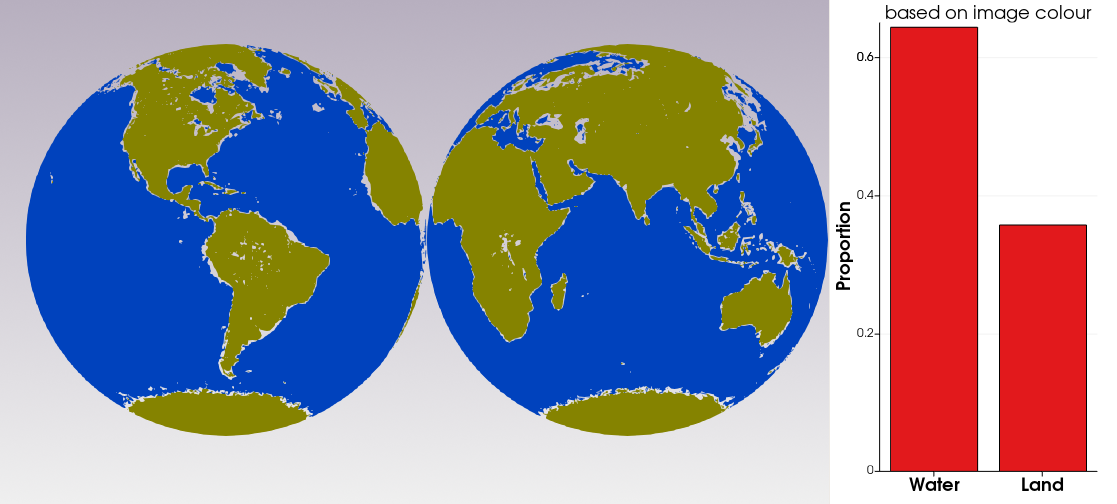
\includegraphics[width=\textwidth]{images/TwoViewsEarth_bar_chart.png}
    \caption{\href{https://fr.wikibooks.org/wiki/Introduction\_\%C3\%A0\_ParaView/Quelques_exemples_simples}{\underline{Earth}}}
    \label{fig:TwoViewsOfEarth}
    \end{figure}

    \vskip -12pt

\end{column}
    \end{columns}
    
\end{frame}{}

\begin{frame}{Visualisation terminology}

\begin{itemize}
    \item Different sub-fields of visualisation
    \item Scientific visualisation
    \begin{itemize}
        \item discipline of computer science
        \item visualisation of scientific and engineering data-sets
    \end{itemize}{}
    \item Scientific visualisation touches on a number of areas:
    \begin{itemize}
        \item data representations
        \item data processing algorithms
        \item visual representations
        \item user interfaces
    \end{itemize}{}
\end{itemize}{}
    
\end{frame}{}

\begin{frame}{Visualisation Terminology}
    \begin{columns}[t]
    \begin{column}{0.5\linewidth}
    \small
    \begin{itemize}
        \item {\it Data visualisation} -- includes data from other sources, such as financial, marketing, business
        \item Sometimes involves statistical analysis and other analysis techniques not employed in scientific visualisation
        \item Can you think of an example of financial information we might want to visualise?
        \item So we might say that scientific visualisation is a type or subset of data visualisation
    \end{itemize}{}
    
    \end{column}
    
    \begin{column}{0.5\linewidth}
    
    \begin{figure}
        \centering
        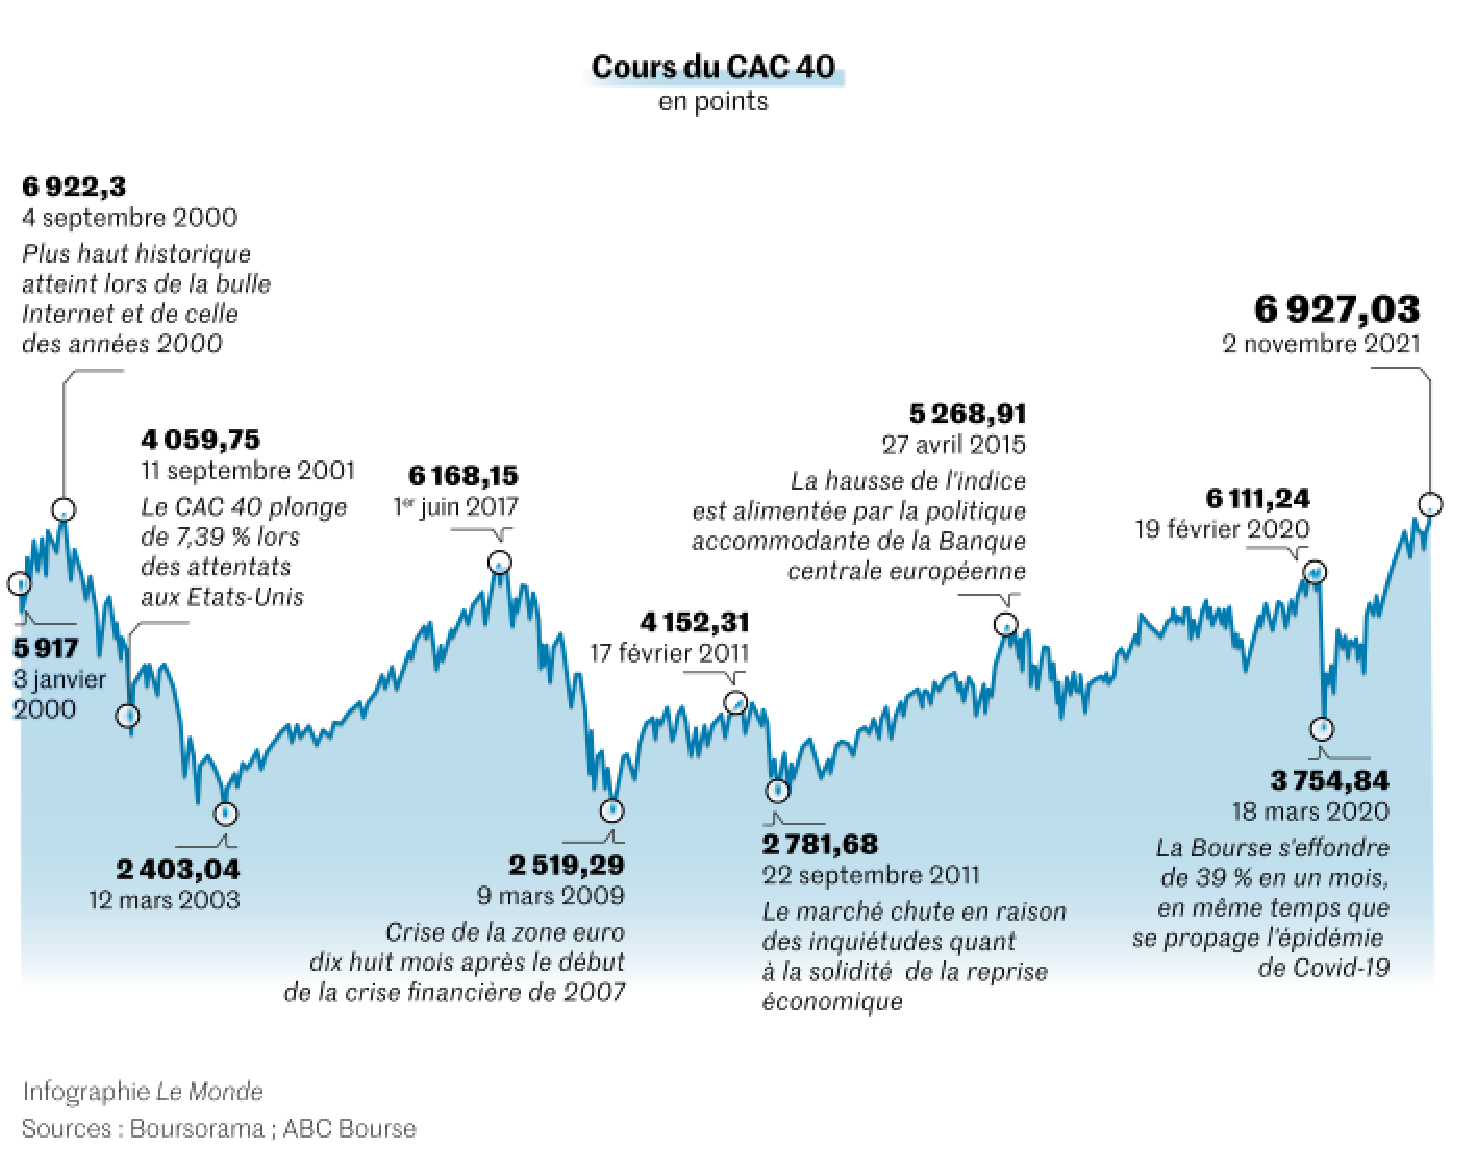
\includegraphics[width=1.1\textwidth]{CAC40.pdf}
        \caption{Cours du CAC 40 en points}
        \label{fig:my_label}
    \end{figure}
    
    \end{column}
    \end{columns}
\end{frame}{}

\begin{frame}{Motivation}

    \begin{columns}[t]
    \begin{column}{0.5\linewidth}
    
    \begin{itemize}
    \item Make sense of huge data-sets
    \begin{itemize}
        \item Computational fluid dynamics produces very large data-sets
    \end{itemize}{}
    \item Uncover insights hidden in the data
    \item Extract important features and meaningful knowledge of the data to assist in the decision-making process
    \end{itemize}{}

    \end{column}
    
    \begin{column}{0.5\linewidth}
    
    \begin{figure}
    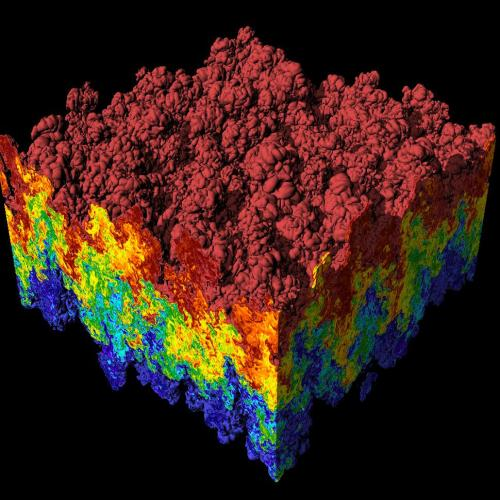
\includegraphics[width=0.9\textwidth]{Rayleigh-Taylor_instability.jpg}
    \caption{Rayleigh-Taylor instability simulation with up to $3072^3$ cells}
    \end{figure}
    
    \end{column}
    
    \end{columns}
    
\end{frame}{}

\begin{frame}{2D example: Flow map}
    
    \begin{itemize}
        \item Show the movement of objects from one location to another
        \item Demonstrates route, size of army and return temperature
    \end{itemize}{}
    
    \begin{figure}
    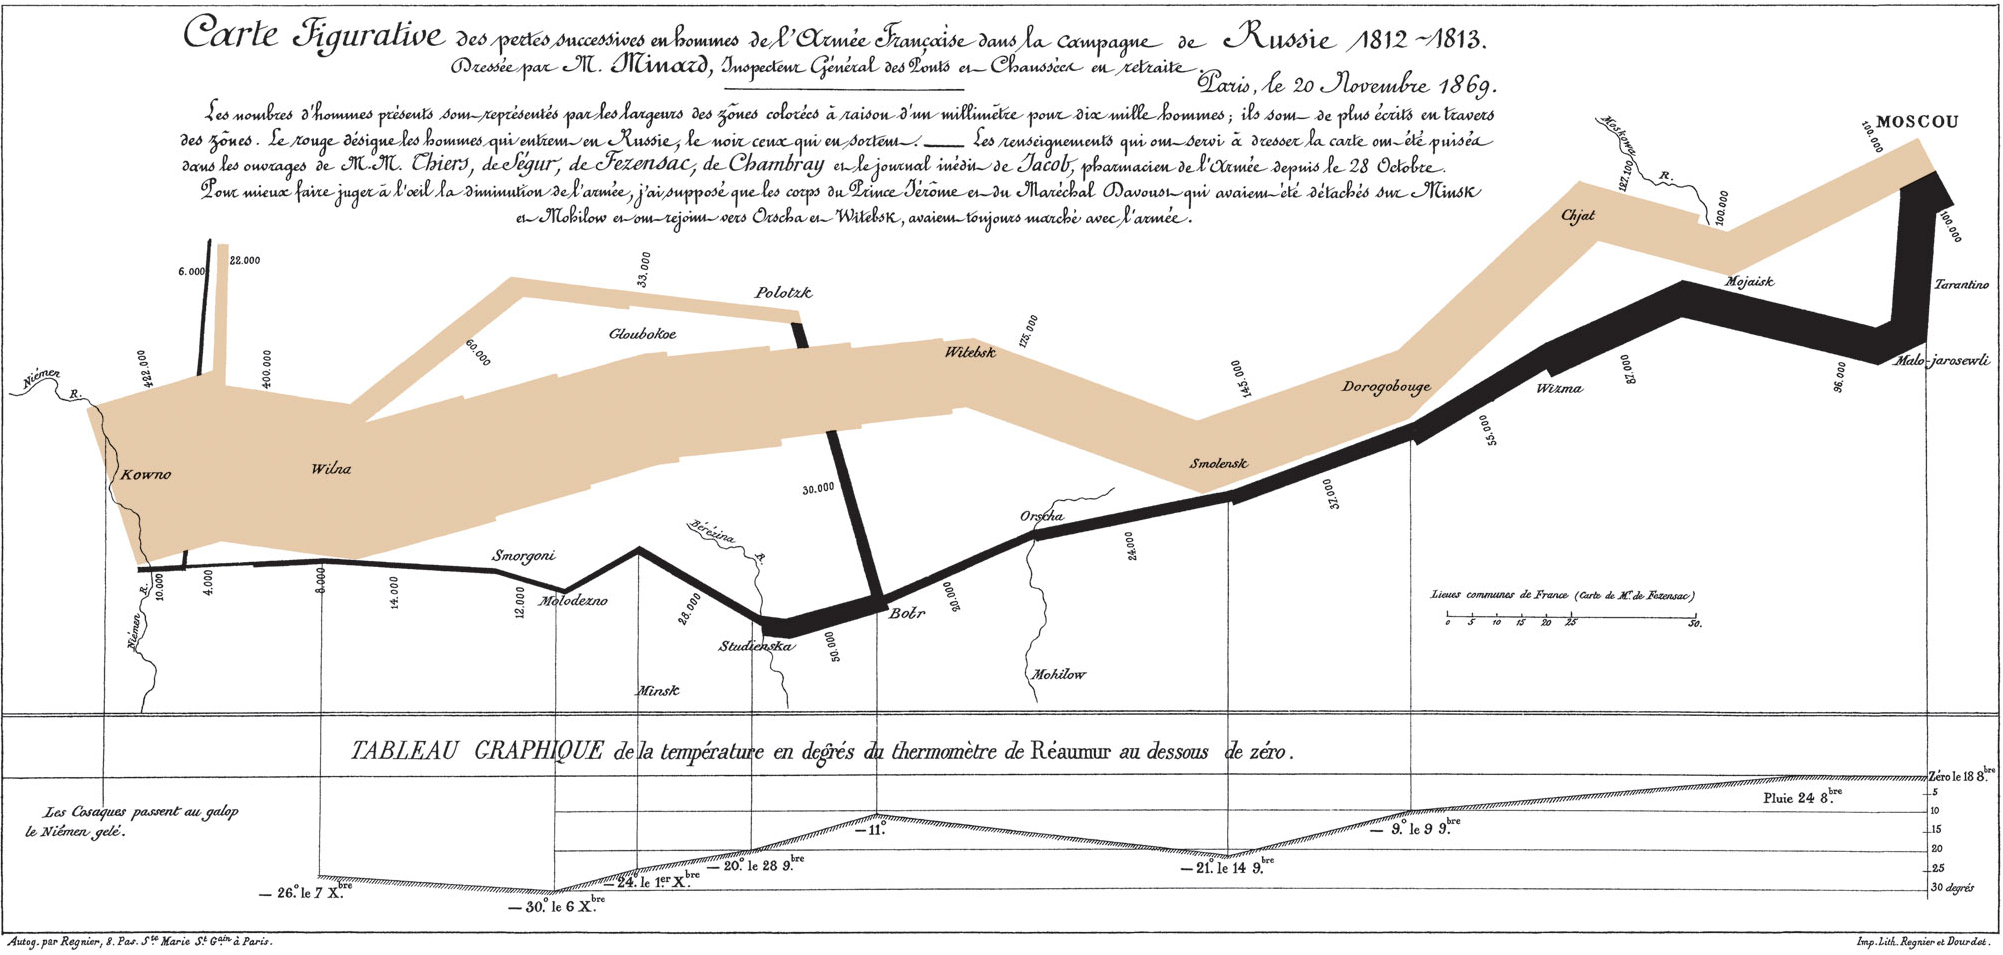
\includegraphics[width=\textwidth]{images/Minard.png}
    \caption{Charles Minard's flow map of Napoleon's March.}
    \label{fig:Minard}
    \end{figure}

\end{frame}{}

\begin{frame}{2D example: Dot style}
    
    \begin{columns}[t]
    \begin{column}{0.5\linewidth}
    
    Visualise disease (cholera) outbreak and find causes
    \begin{itemize}
        \item Cases clustered around pump in Broad (now Broadwick) street
        \item Water for the pump was polluted by sewage from nearby cesspit
    \end{itemize}
    \end{column}
    
    \begin{column}{0.5\linewidth}
    
    \begin{figure}
    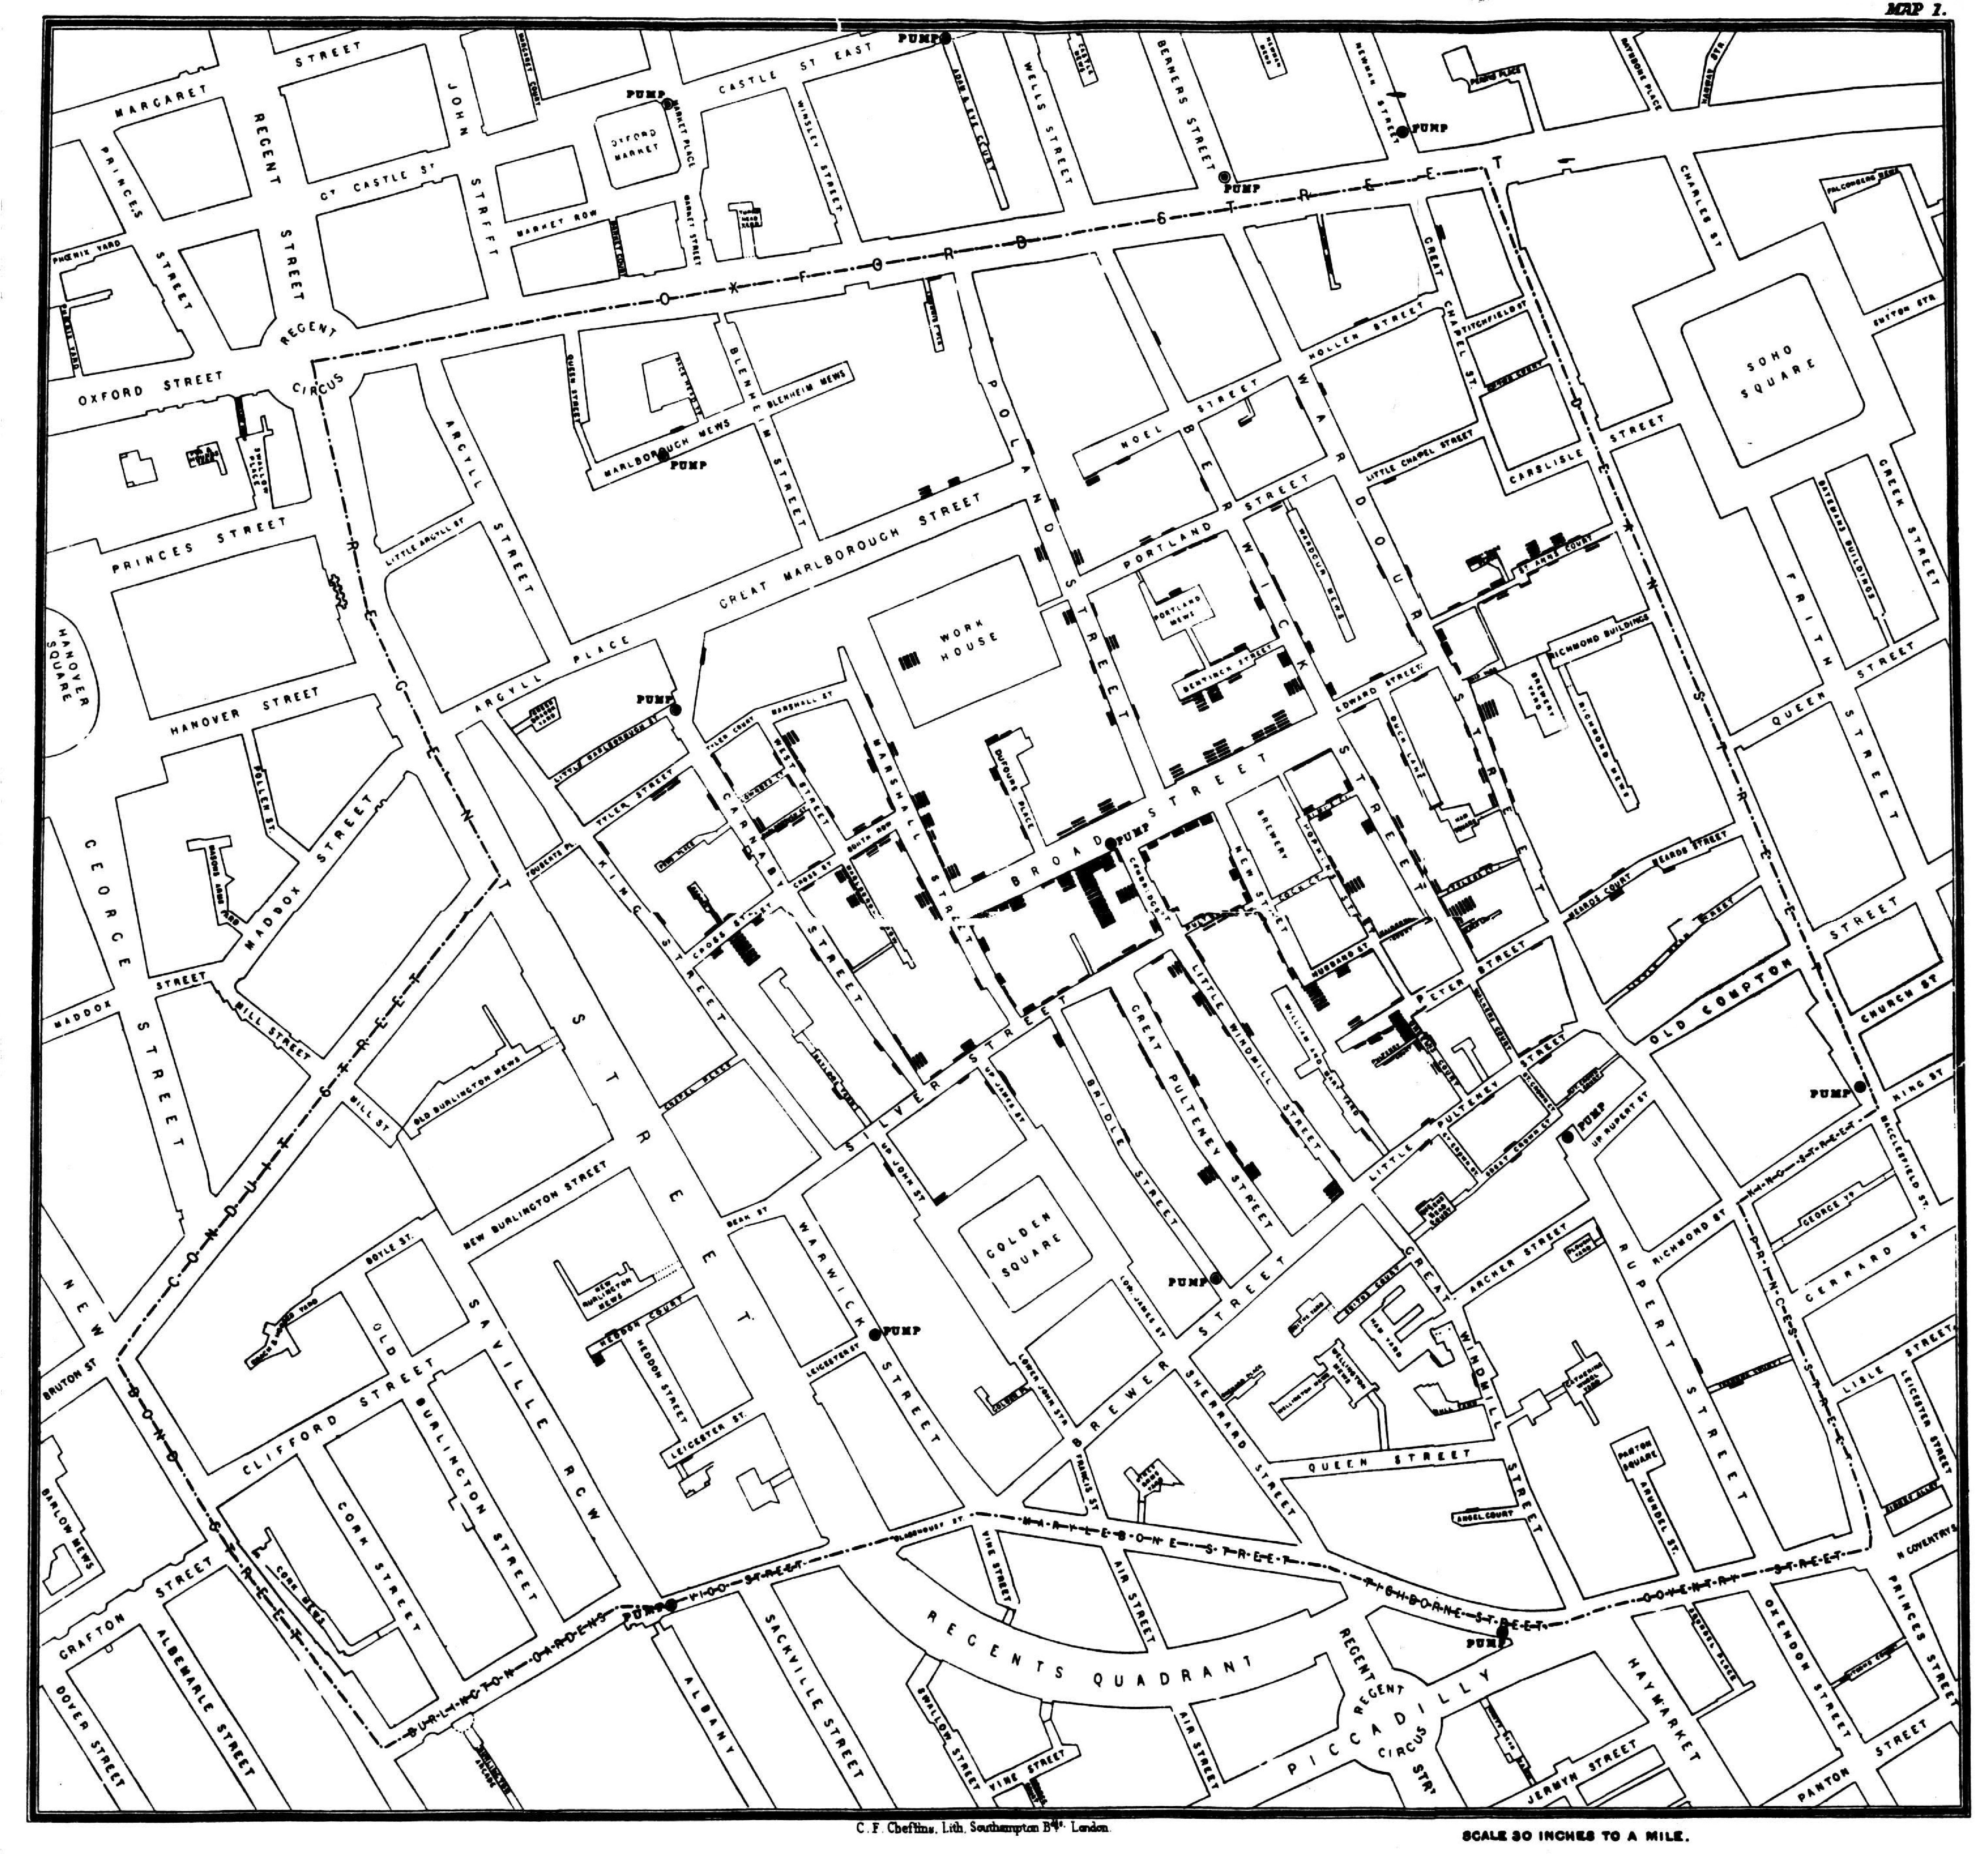
\includegraphics[width=\textwidth, trim={350 500 500 500}, clip]{images/Snow-cholera-map-1.pdf}
    \caption{John Snow's Cholera map in dot style, 1854.}
    \label{fig:Snow}
    \end{figure}
    
    \end{column}
    
    \end{columns}
    
\end{frame}{}

\section{Introduction to ParaView}

\begin{frame}{Introduction : ParaView}

\begin{itemize}
    \item Open-source, scalable, multi-platform visualisation application
    \item Data parallelism on shared-memory or distributed-memory multi-computers and clusters
    \item An open, flexible, and intuitive user interface
    \item An extensible, modular architecture based on open standards
    \item Large user community, both public and private sector
    \item A flexible BSD 3 Clause license
\end{itemize}{}

\vskip 12pt

Downloaded roughly 100,000 times a year \qquad Won many awards

\end{frame}


\begin{frame}{Introduction : ParaView examples}

\vskip -12pt

    \begin{columns}[t]
    \begin{column}{0.45\linewidth}
    \begin{figure}
    \centering
    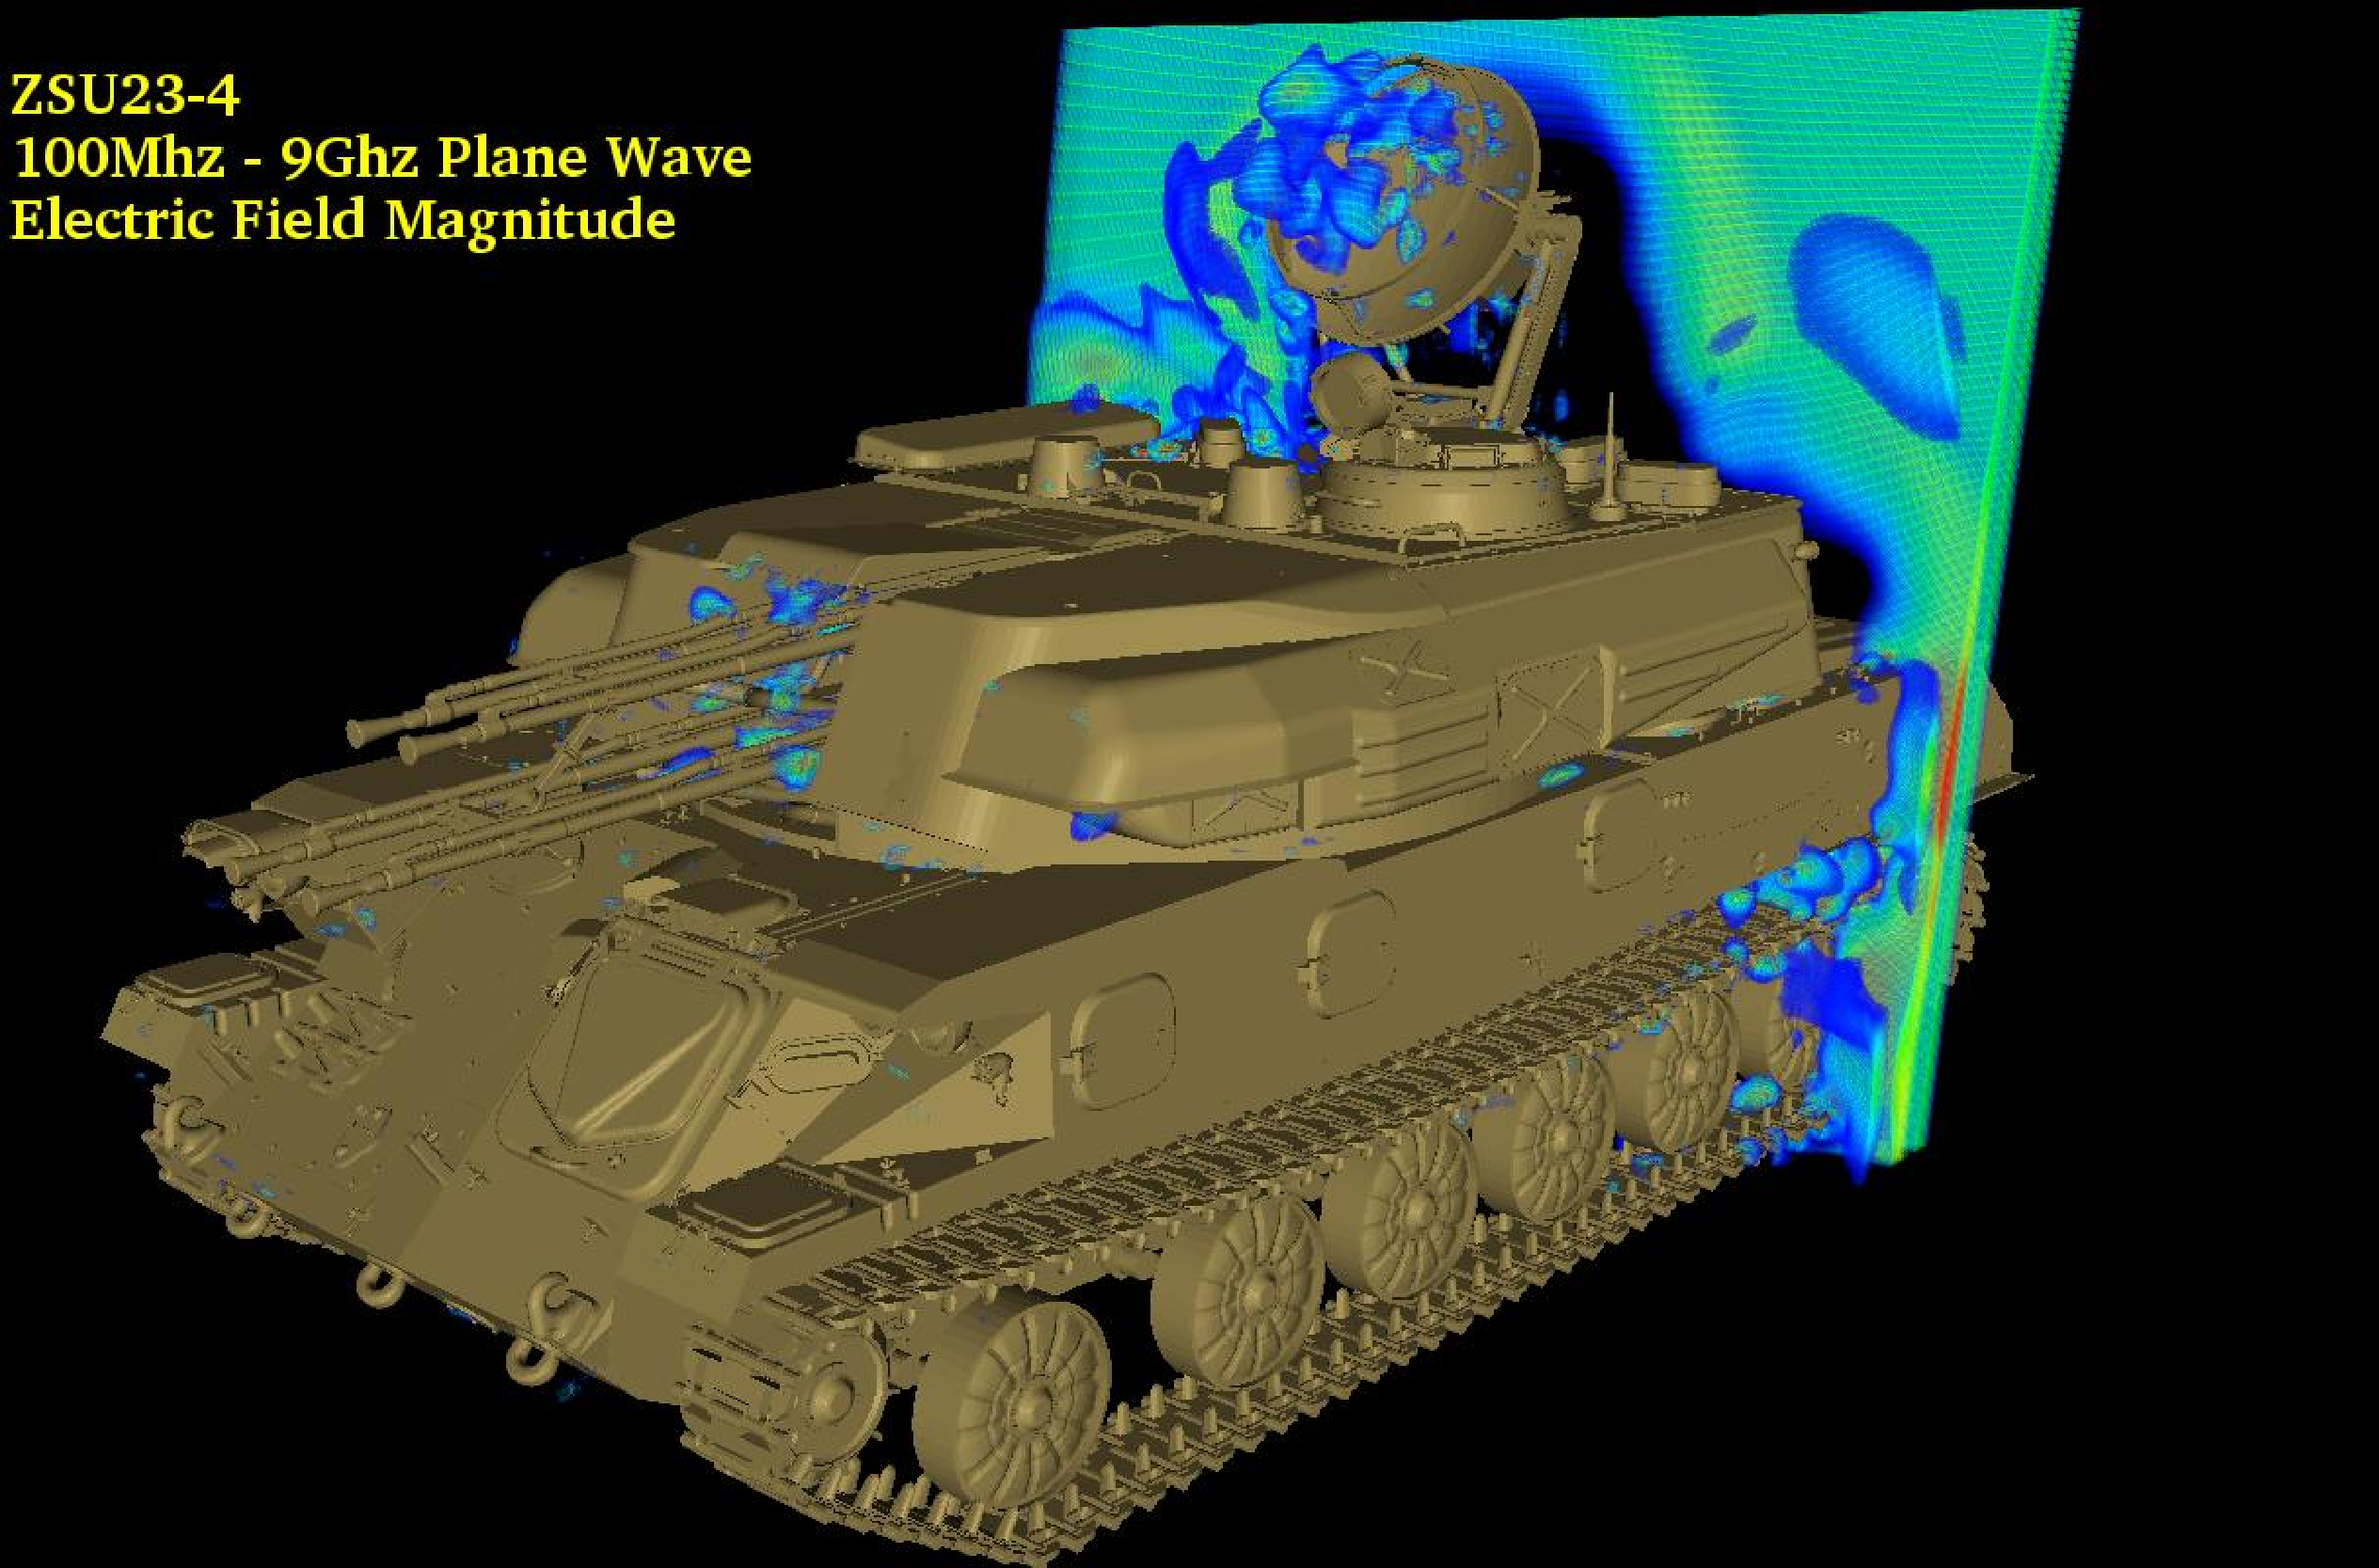
\includegraphics[height=0.5\textwidth]{images/RussianAntiAircraft_ZSU23-4.pdf}
    \captionsetup{labelformat=empty}
    \caption{\tiny ZSU23-4 Russian Anti-Aircraft vehicle being hit by a planar wave. Image courtesy of Jerry Clarke, US Army Research Laboratory.}
    \label{fig:RussianAntiAircraft_ZSU23}
    \end{figure}
    
    \vskip -20pt
    
    \begin{figure}
    \centering
    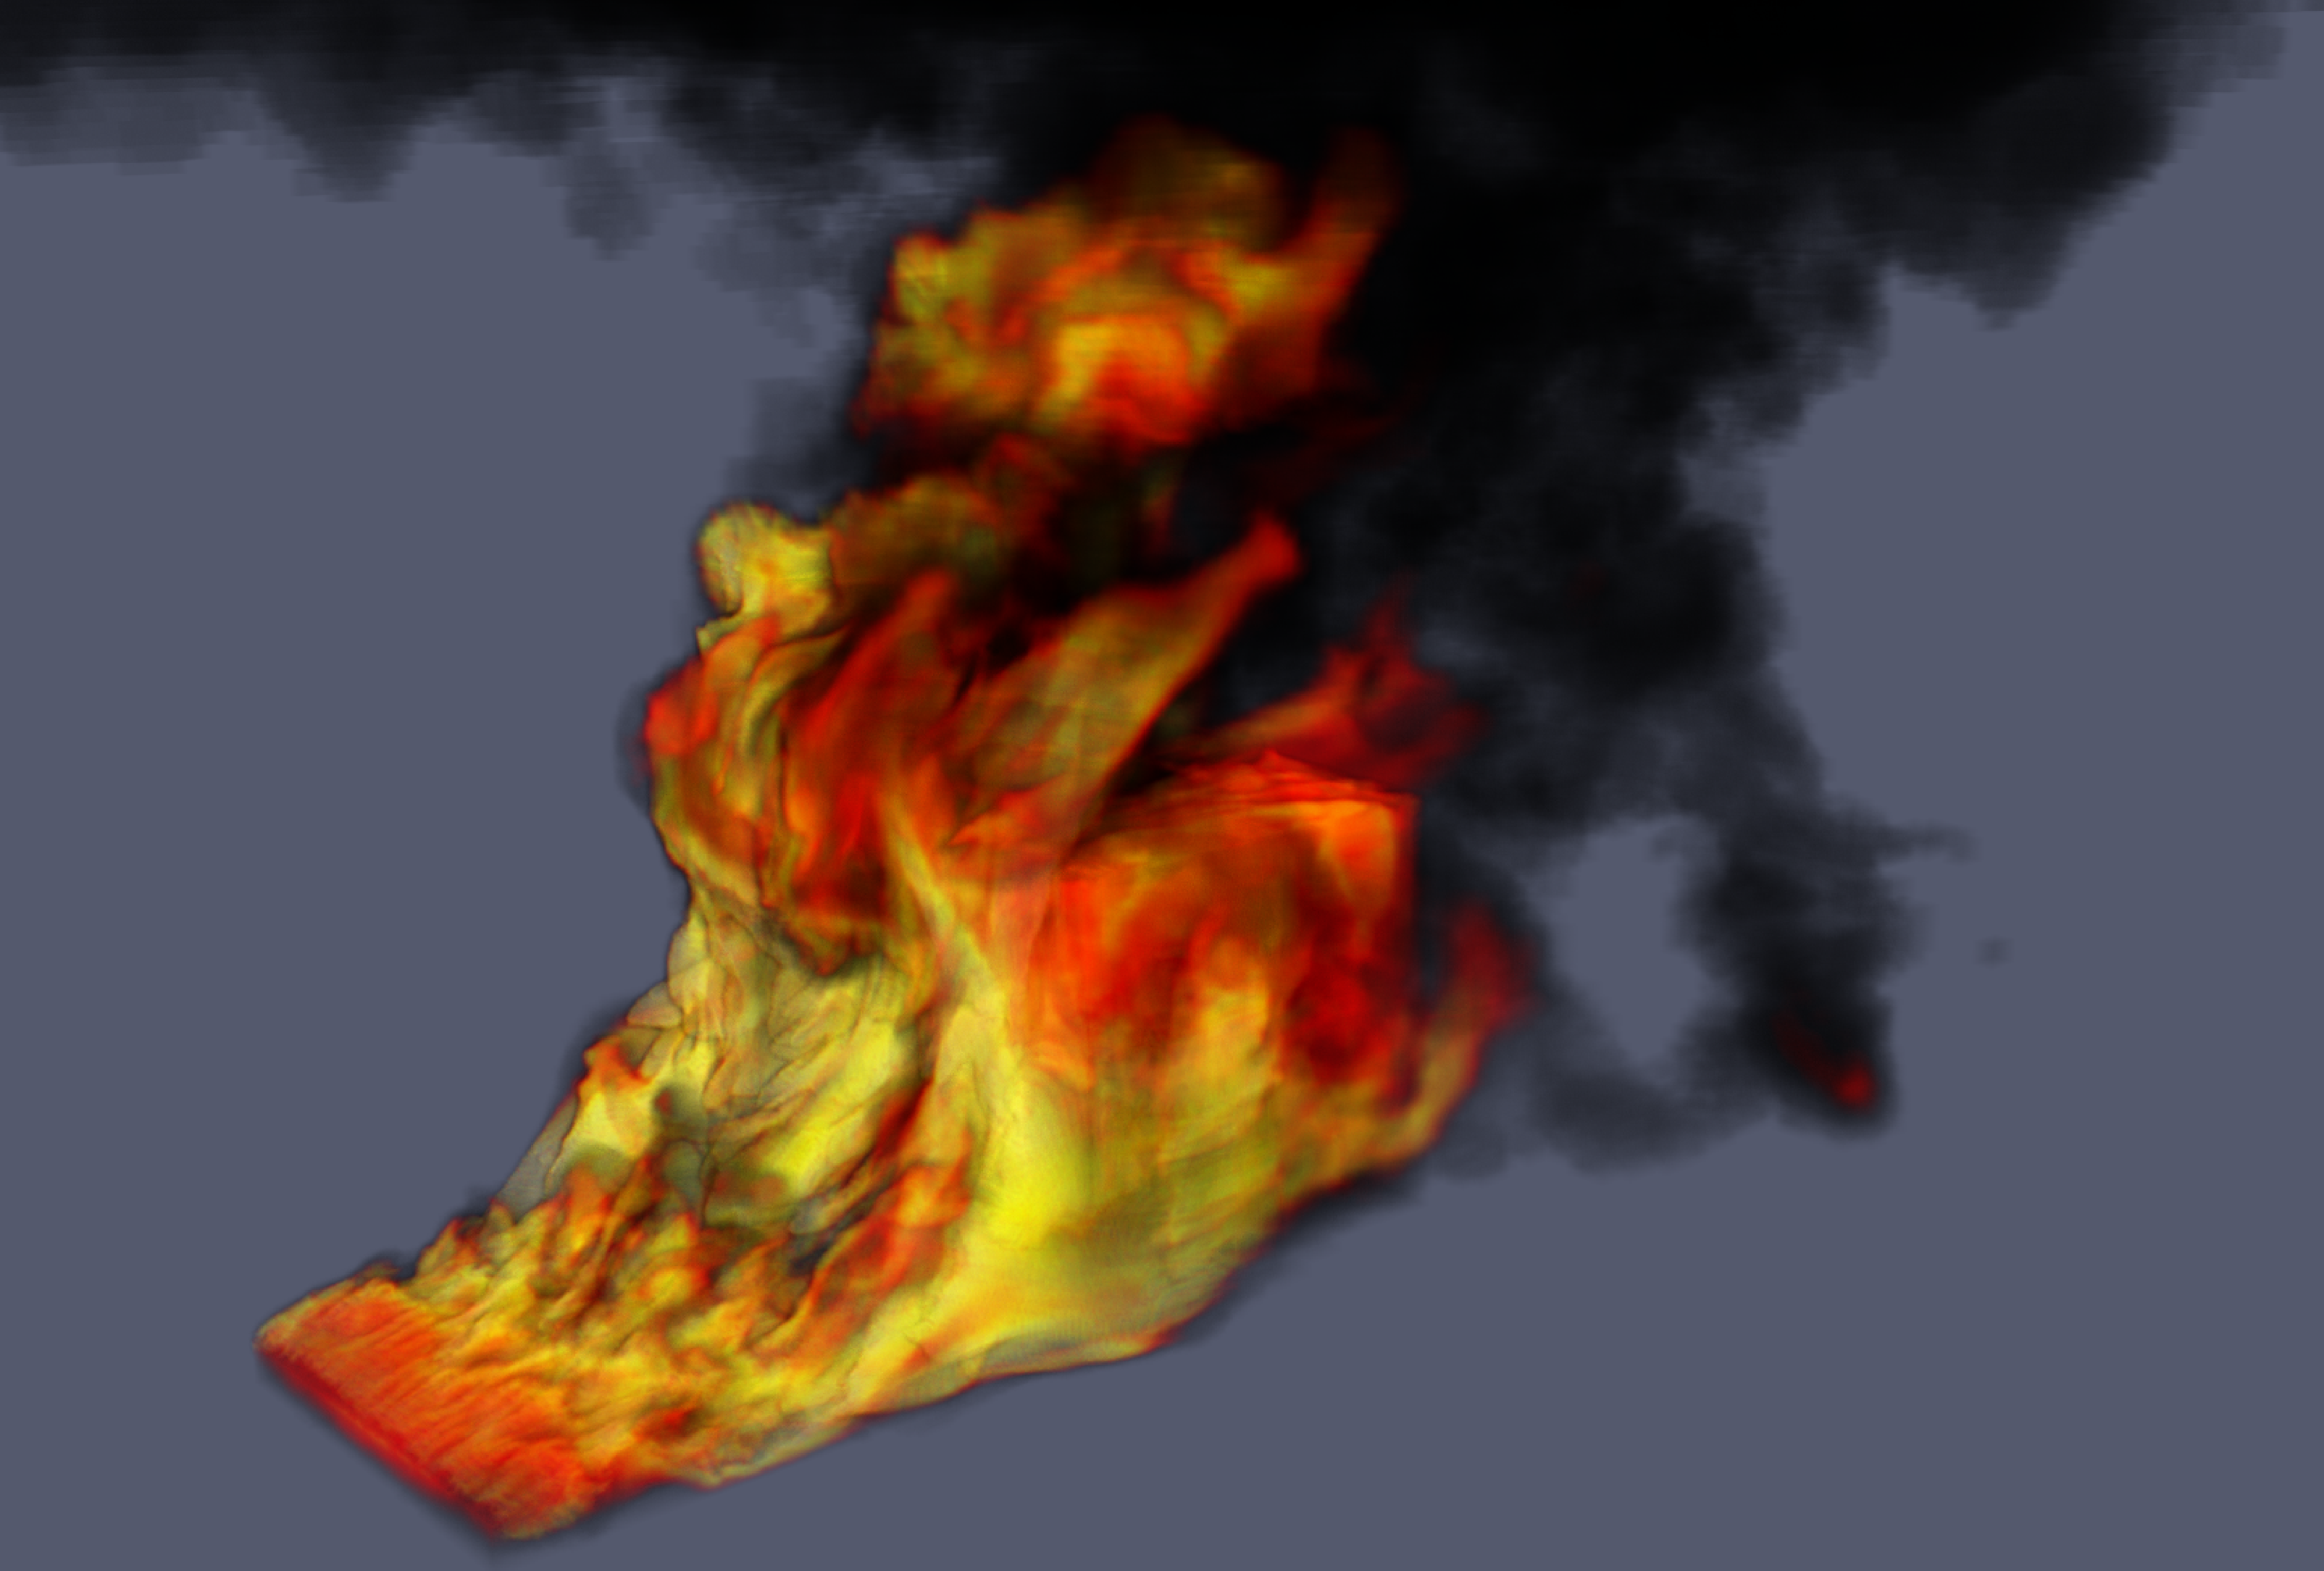
\includegraphics[height=0.5\textwidth]{images/CrosswindFire.pdf}
    \captionsetup{labelformat=empty}
    \caption{\tiny A loosely coupled SIERRA-Fuego-Syrinx-Calore simulation with 10 million unstructured hexahedra cells of objects-in-crosswind fire.}
    \label{fig:CrosswindFire}
    \end{figure}
    \end{column}
    
    \begin{column}{0.45\linewidth}
   
    \begin{figure}
    \centering
    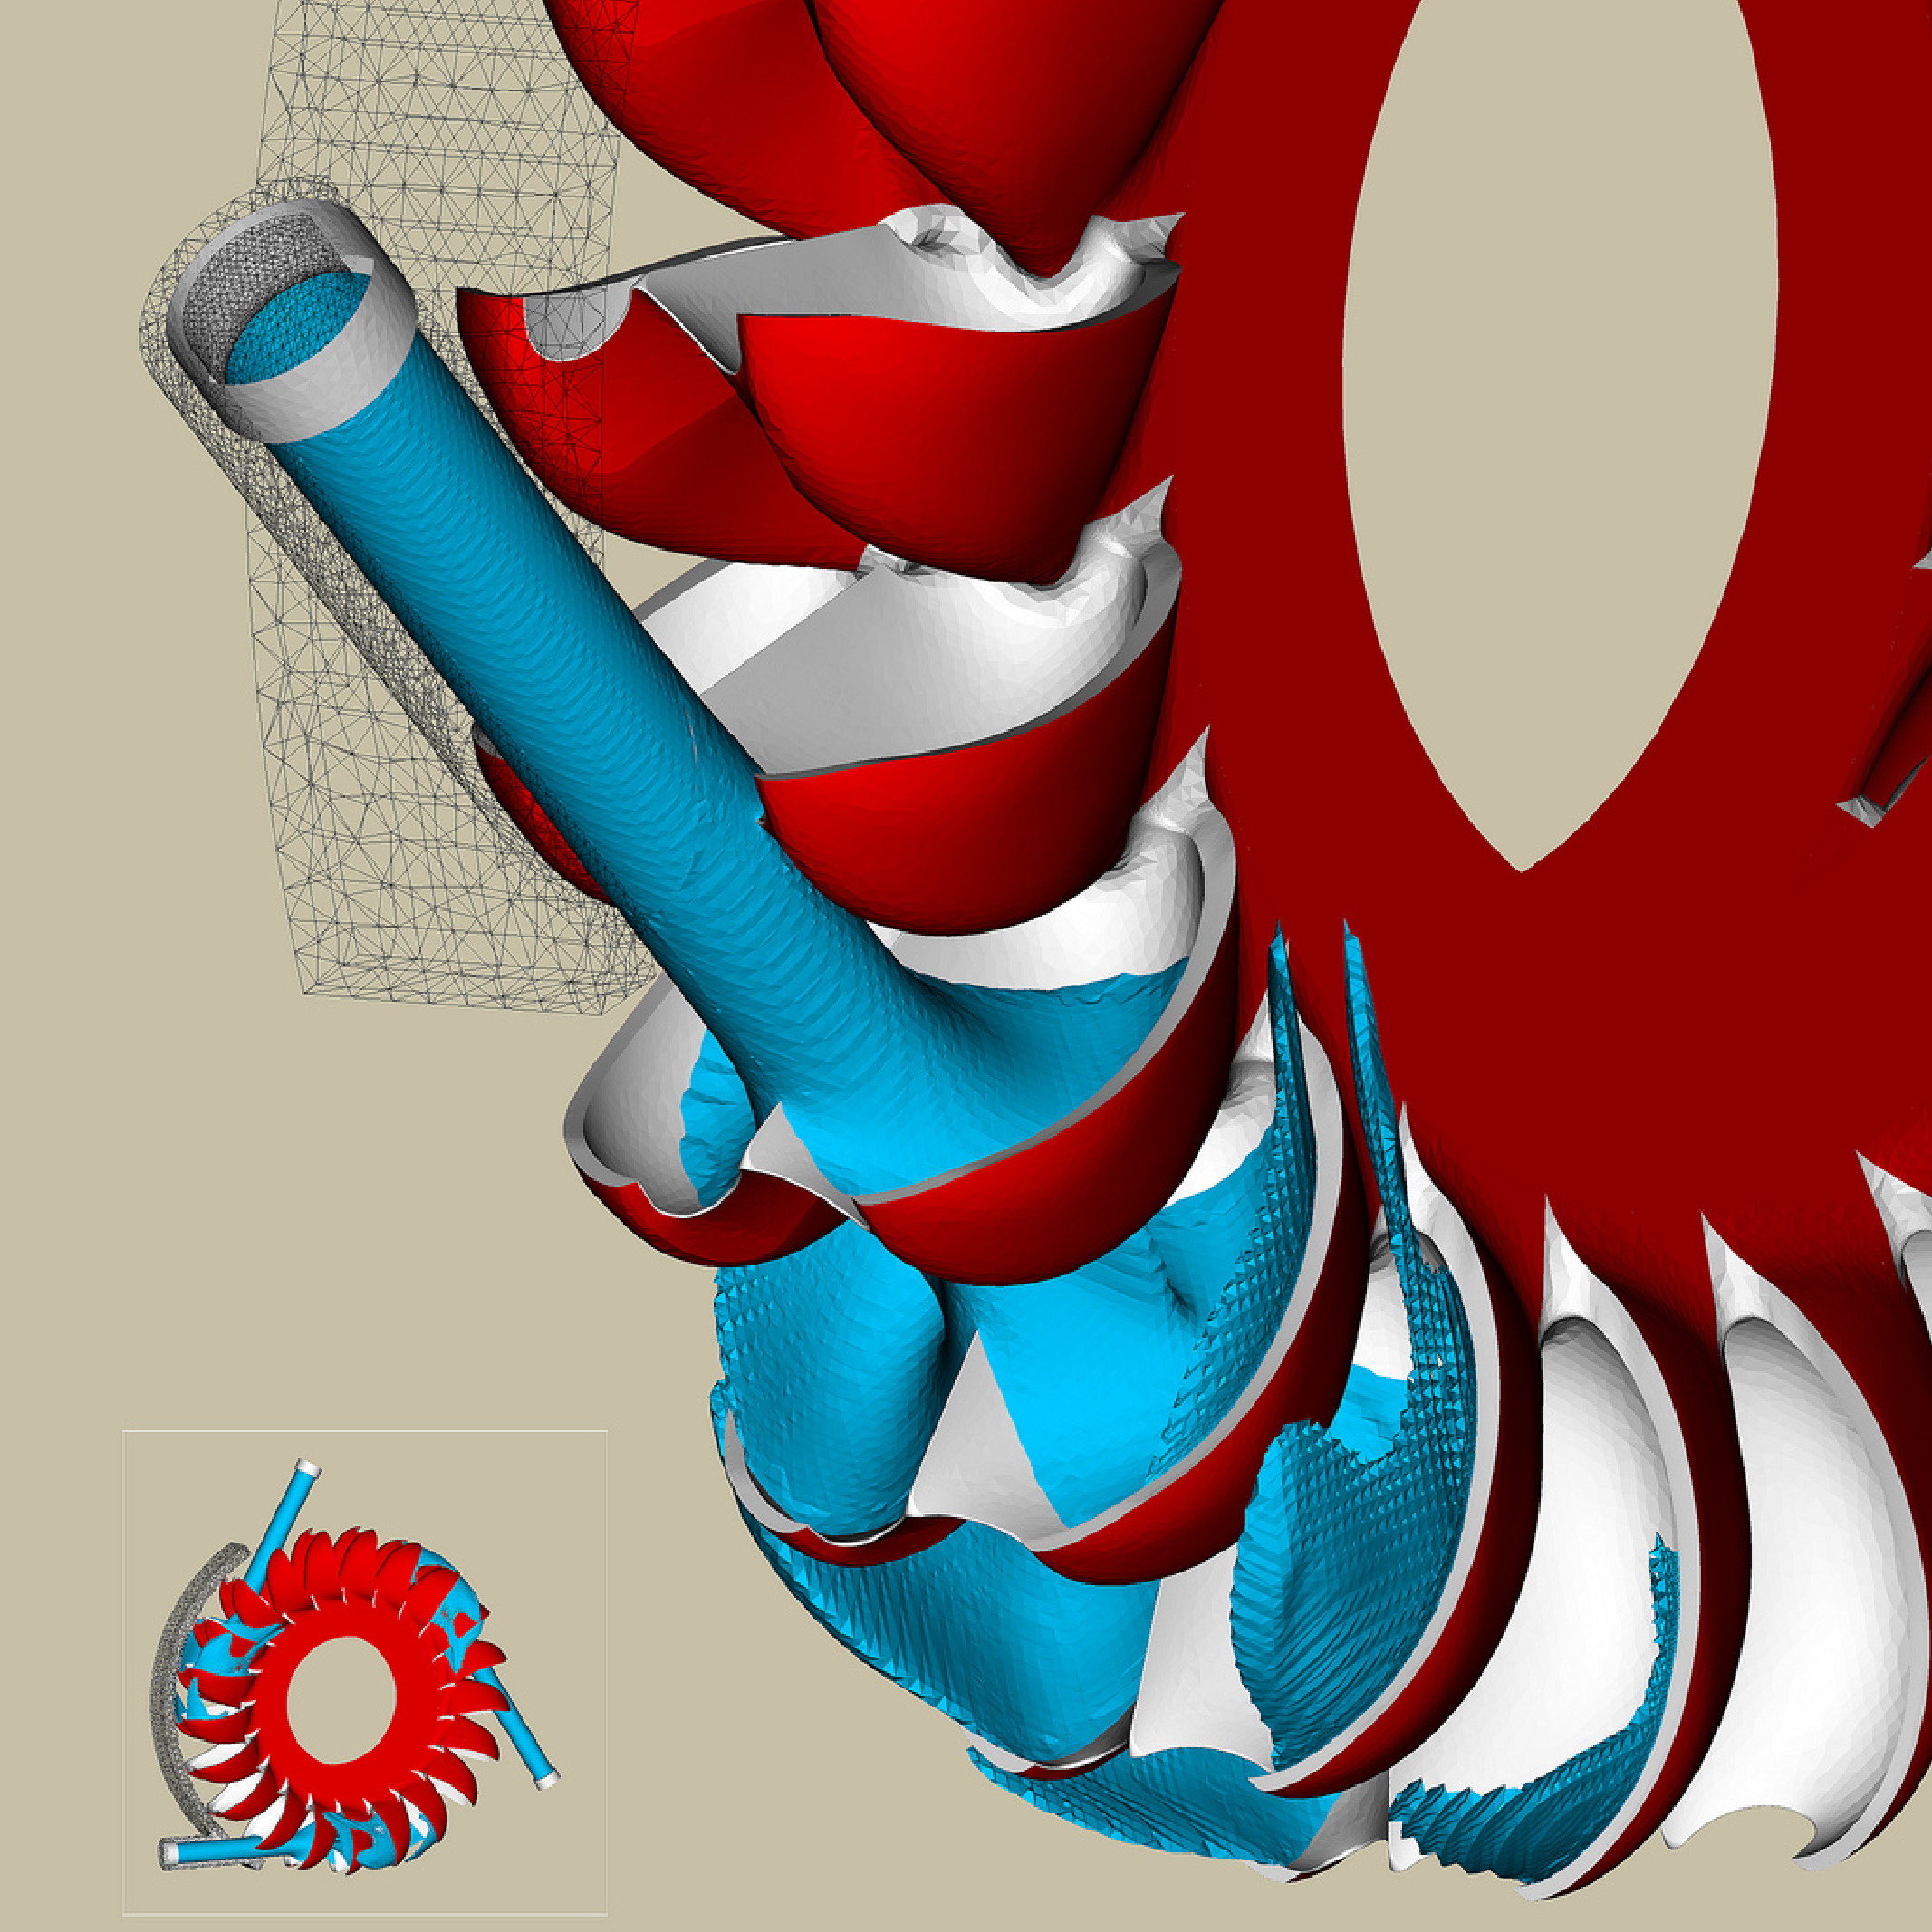
\includegraphics[height=0.5\textwidth]{images/Pelton.pdf}
    \captionsetup{labelformat=empty}
    \caption{\tiny Simulation of a Pelton turbine. Image courtesy of the Swiss National Supercomputing Centre}
    \label{fig:Pelton}
    \end{figure}
 
    \vskip -20pt
    
    \begin{figure}
    \centering
    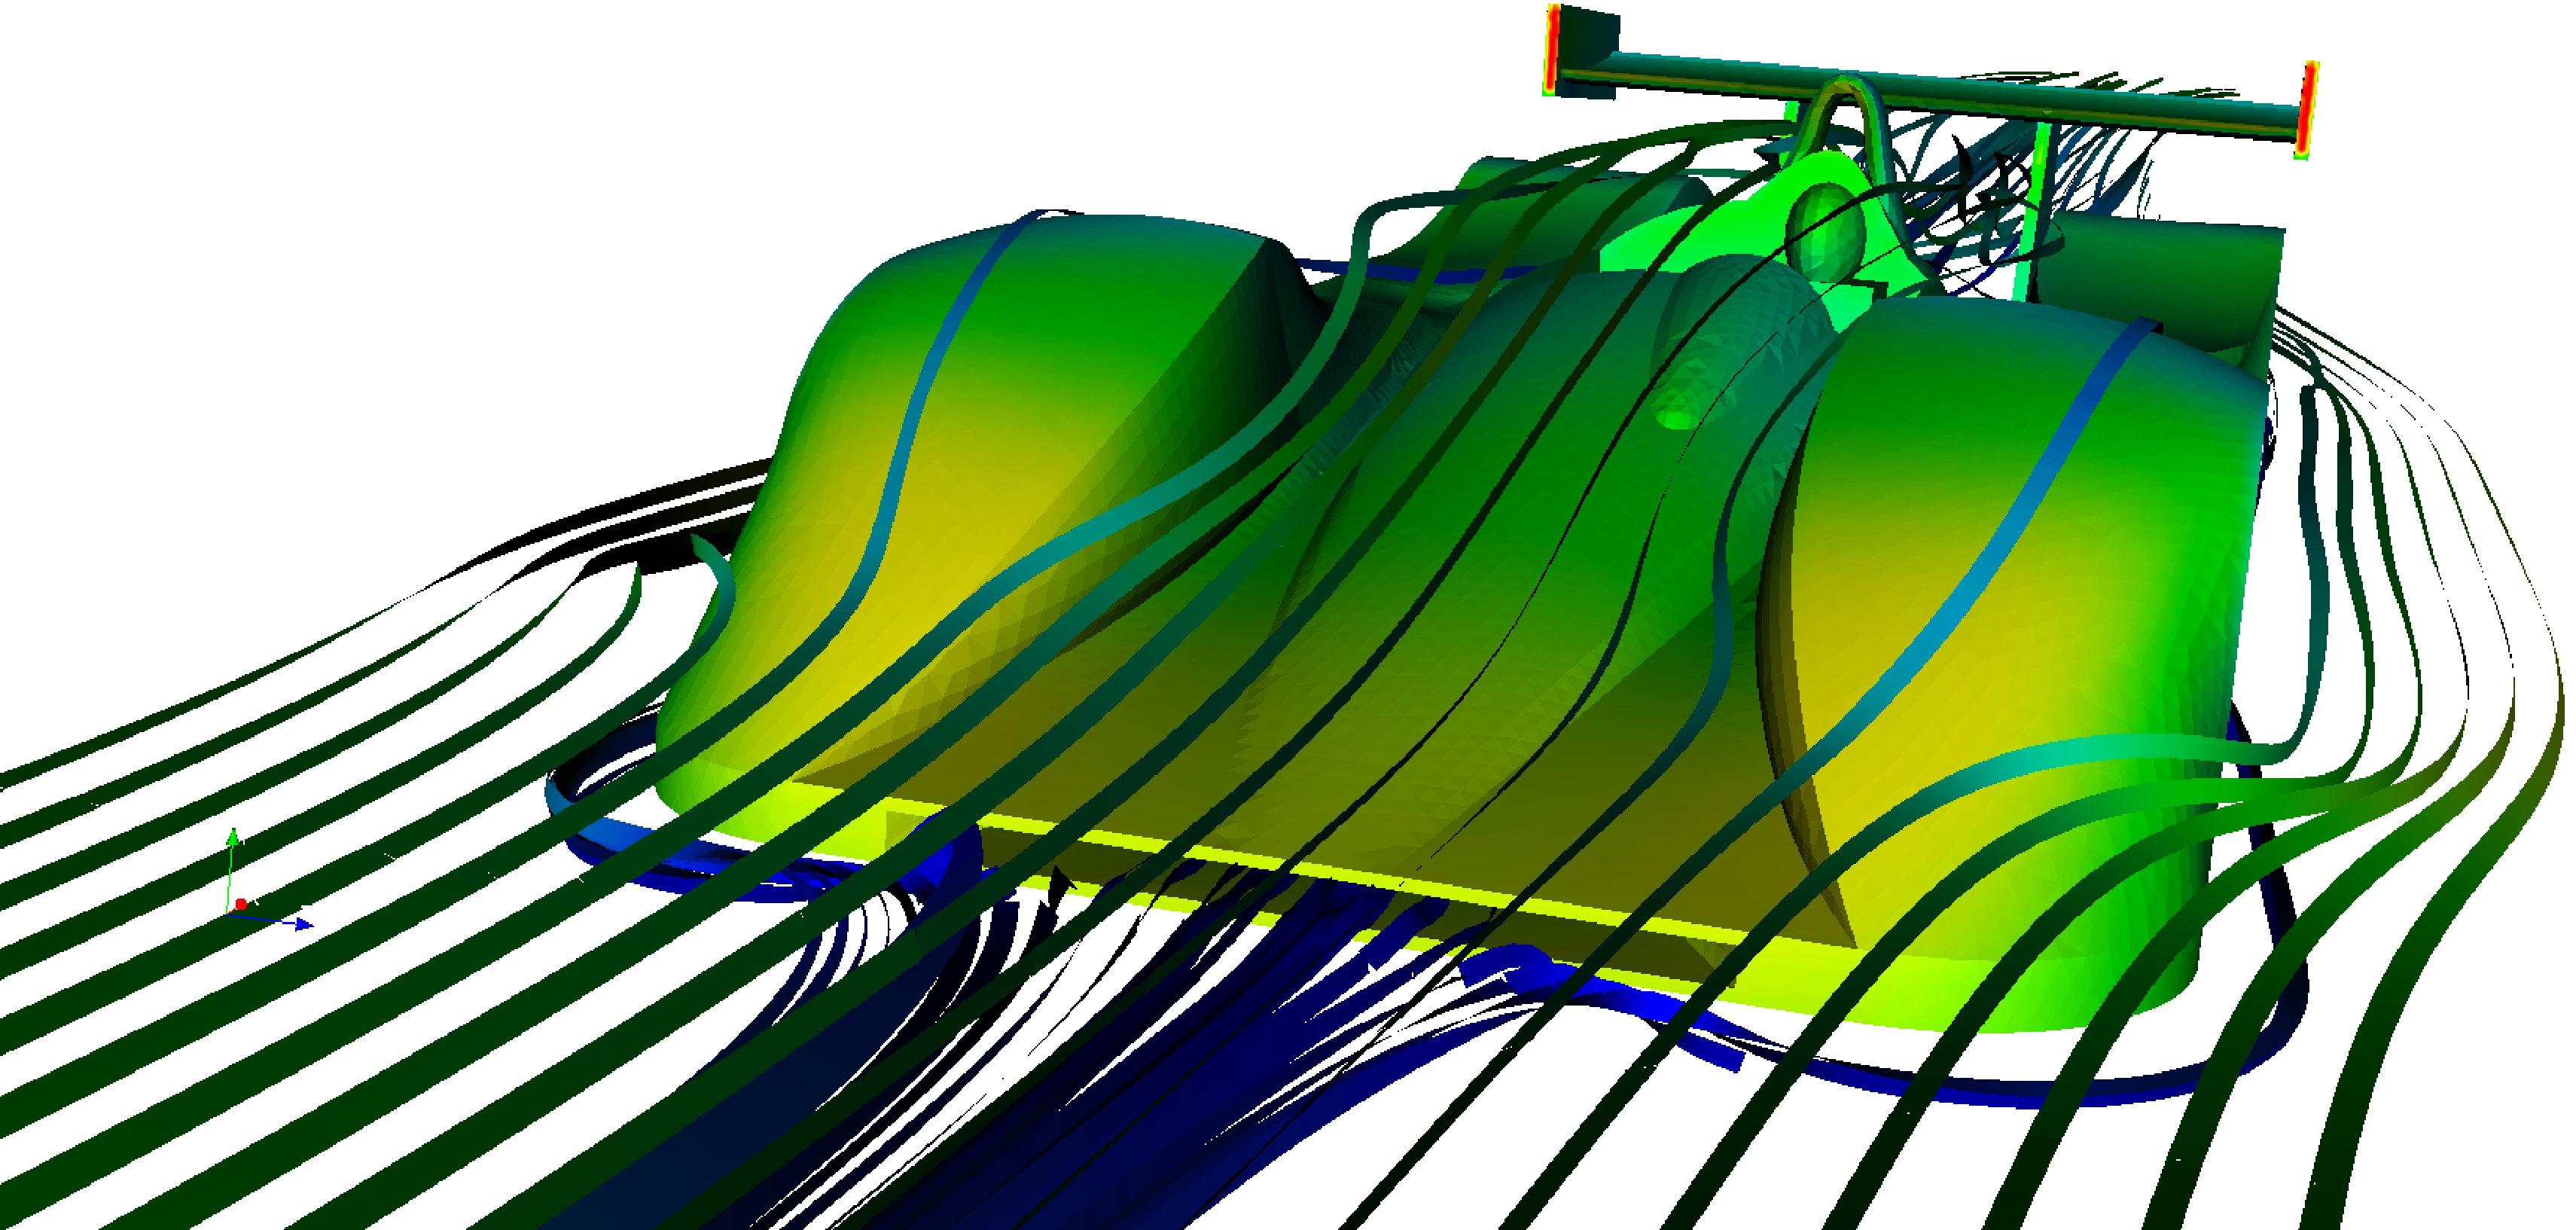
\includegraphics[height=0.5\textwidth]{images/LeMans.pdf}
    \captionsetup{labelformat=empty}
    \caption{\tiny Airflow around a Le Mans Race car. Image courtesy of Renato N. Elias, NACAD/COPPE/UFRJ, Rio de Janerio, Brazil}
    \label{fig:LeMans}
    \end{figure}
    
    \end{column}
    \end{columns}

\end{frame}{}

\begin{frame}{Introduction : ParaView application Architecture}

    \begin{figure}
    \centering
    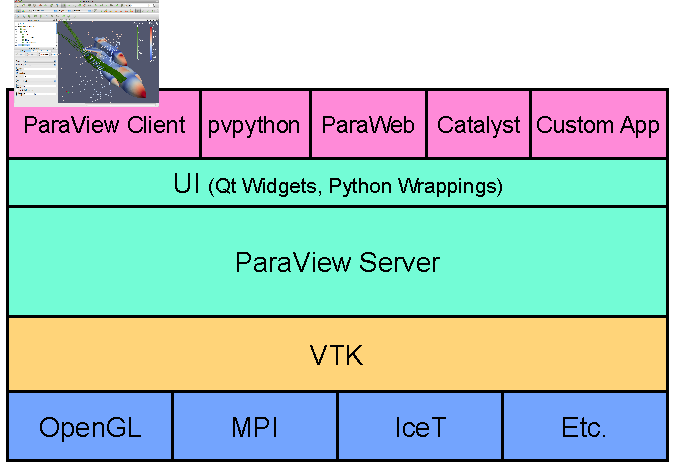
\includegraphics[height=0.5\textwidth]{images/ParaViewLibStack.pdf}
    \captionsetup{labelformat=empty}
    \caption{}
    \label{fig:ParaViewLibStack}
    \end{figure}
    
    \vskip -24pt
    
    \begin{itemize}
        \item ParaView is just a small client application built on top of a tall stack of libraries
        \item pvpython allows automation of post-processing
    \end{itemize}{}
    
\end{frame}{}

\begin{frame}{Introduction : VTK library}
    
    Visualization Toolkit (VTK) is an open-source, freely available software system for :
    \begin{itemize}
        \item 3D computer graphics, modelling, image processing, volume rendering, {\bf scientific visualisation}, 2D plotting
    \end{itemize}{}
    
    \vskip 6pt
    
    Filters :
    \begin{itemize}
        \item VTK applications manipulate data with filters
        \item inspect received data and produces derived data
    \end{itemize}{}
    
    \vskip 6pt
    
    Multiple applications, e.g. open source platforms include :
    \begin{itemize}
        \item The {\bf Insight Segmentation and Registration Toolkit (ITK)}; algorithms for medical research
        \item {\bf ParaView} works with data on the desktop, on the web, on supercomputers, in immersive environments and more
        \item \href{https://docs.pyvista.org/index.html}{\bf PyVista} 3D plotting and mesh analysis
        \item {\bf 3D Slicer} is an extensible platform for visualisation and medical image analysis
    \end{itemize}{}
    
\end{frame}{}

\begin{frame}{ParaView Interface}

    \begin{figure}
    \centering
    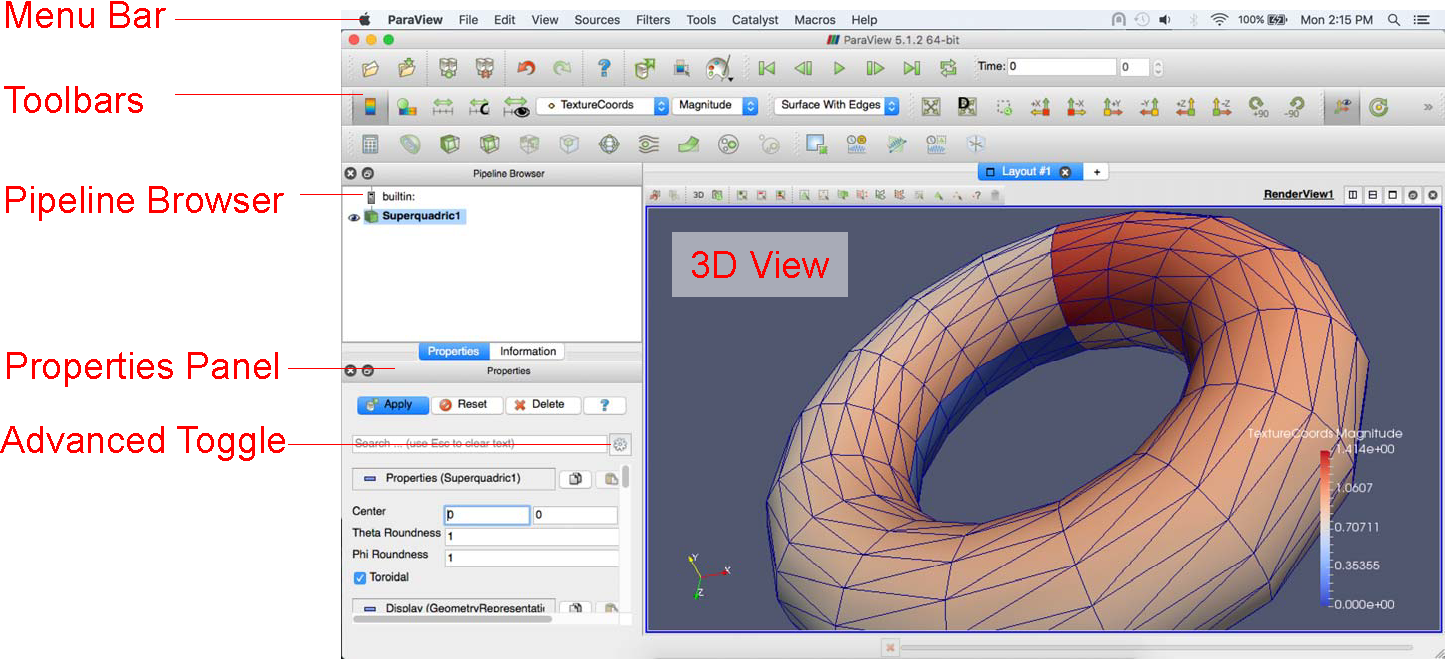
\includegraphics[height=0.4\textwidth]{images/UserInterface.pdf}
    \captionsetup{labelformat=empty}
    \label{fig:UserInterface}
    \end{figure}
    
    \vskip -10pt
    
    \footnotesize
    
    \begin{description}
        \item[Menu Bar] Allows access to majority of features
        \item[Toolbars] Provides quick access to most commonly used features
        \item[Pipeline Browser] ParaView manages the reading and filtering of data with a pipeline. Browser allows the pipeline structure and select pipeline objects to be viewed
        \item[Properties Panel] Allows viewing and changing of parameters for current pipeline object
        \item[3D View] Used to present data so that you may view, interact with, and explore data
    \end{description}
    
\end{frame}{}

\section{Exercises}

\begin{frame}{Exercise 1: ParaView line plot}
    
    \begin{columns}[c]
    \begin{column}{0.45\linewidth}
    \begin{itemize}
        \item Create \texttt{.csv} file (right)
        \item \texttt{File}$\rightarrow$ \texttt{Open}, \texttt{OK} \& \texttt{Apply}
        \item \texttt{[ctrl] + [space]}, and search for \texttt{Plot Data}, & \texttt{Apply}
        \item Change $x$-axis parameter
    \end{itemize}{}
    \end{column}
    
    \begin{column}{0.45\linewidth}
    
    \texttt{\small"x", "y"\newline
    0  , 0\newline
    1  , 1\newline
    2  , 4\newline
    3  , 9\newline
    4  , 16\newline
    5  , 25\newline
    6  , 36\newline
    7  , 49}
    
    \end{column}
    \end{columns}
    
\end{frame}{}

\begin{frame}{Sources}
    Two ways to get data into ParaView:
    \begin{itemize}
        \item Read data from a file
        \item Generate data with a {\bf source} object
    \end{itemize}
    
\vskip 24pt

Exercise; Open ParaView, then \texttt{Sources $\rightarrow$ Cylinder}, \texttt{Apply}
\vskip 12pt
\centering{

\includegraphics[width=0.15\textwidth]{Apply.png}
}

\vskip 12pt

    After, increase the cylinder resolution. Manipulate the cylinder in the viewing window. Continue by demonstrating basic features of ParaView interface (colours, axes, opacity, auto apply, colour palette).
    
\end{frame}{}




\begin{frame}{Earth visualisation}
    \footnotesize
    
    Familiarisation exercise using the earth example \href{https://fr.wikibooks.org/wiki/Introduction\_\%C3\%A0\_ParaView/Quelques_exemples_simples}{\bf\underline{here}}. Prenons le \href{https://commons.wikimedia.org/wiki/File:Land_ocean_ice_2048.jpg}{\bf\underline{image}}, puis :
    \begin{enumerate}
        \item Ouvrir ParaView
        \item Cliquer sur le bouton \texttt{Open}, et ouvrir le fichier \texttt{Land\_ocean\_ice\_2048.jpg}; \texttt{Apply}.
        \item Faire bouger l'image avec la souris
        \item Cliquer sur le bouton \texttt{Split vertical} (en haut à droite de la fenêtre de visualisation). Dans la fenêtre \texttt{Create View} qui apparaît, cliquer sur le bouton \texttt{Render View}
        \item Sélectionner le menu \texttt{Sources $\rightarrow$ Sphere}. Cliquer sur Apply. Changer les valeurs Theta resollution et Phi resolution sur 16 et \texttt{Apply}
        \item Sélectionner le menu \texttt{Filters $\rightarrow$ Alphabetical $\rightarrow$ Texture Map to Sphere}. \texttt{Apply}
        \item Dans la boîte \texttt{Properties}, cliquer sur \texttt{Toggle advanced properties} \icon{pqAdvanced26}. Dans la zone Lighting (tout en bas), cliquer sur le menu \texttt{Texture} et choisir l'option Load$\dots$
        \item Dans la fenêtre \texttt{Open texture} qui apparaît, aller chercher le fichier \texttt{Land\_ocean\_ice\_2048.jpg} et cliquer sur OK
        \item Dans la boîte \texttt{Properties}, décocher l'option \texttt{Prevent} seam, \texttt{Apply}
    \end{enumerate}
    
    {\it But, this example is not quite perfect...}

    

\end{frame}{}


\begin{frame}{Regular mesh types}
    
    \begin{columns}[t]
    \begin{column}{0.3\linewidth}
    \begin{figure}
    \centering
    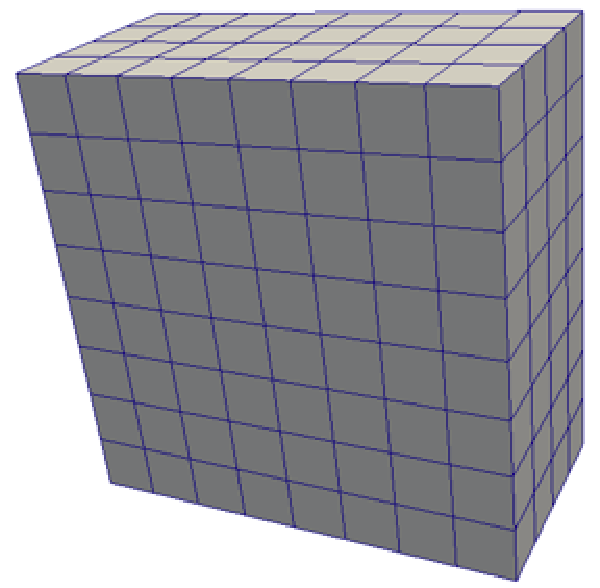
\includegraphics[width=\textwidth]{images/Grids/Rectilinear.pdf}
    \captionsetup{labelformat=empty}
    \caption{\footnotesize Uniform Rectilinear}
    \label{fig:Rectilinear}
    \end{figure}
    \tiny
    A uniform rectilinear grid is a one- two- or three- dimensional array of data. The points are orthonormal to each other and are spaced regularly along each direction.
    
    \end{column}
    
    \begin{column}{0.3\linewidth}
    \begin{figure}
    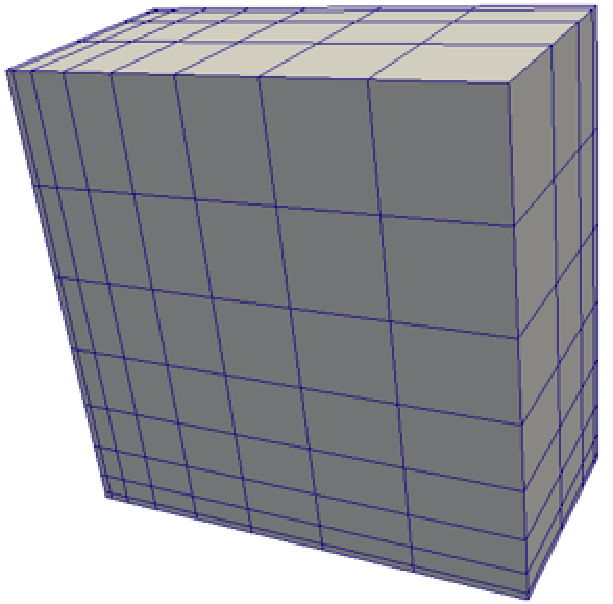
\includegraphics[width=\textwidth]{images/Grids/nonUniRectilinear.pdf}
    \captionsetup{labelformat=empty}
    \caption{\footnotesize Non-uniform Rectilinear}
    \label{fig:nonUniRectilinear}
    \end{figure}
    \tiny
    Similar to the uniform rectilinear grid except that the spacing between points may vary along each axis.
    \end{column}

    \begin{column}{0.3\linewidth}
    \begin{figure}
    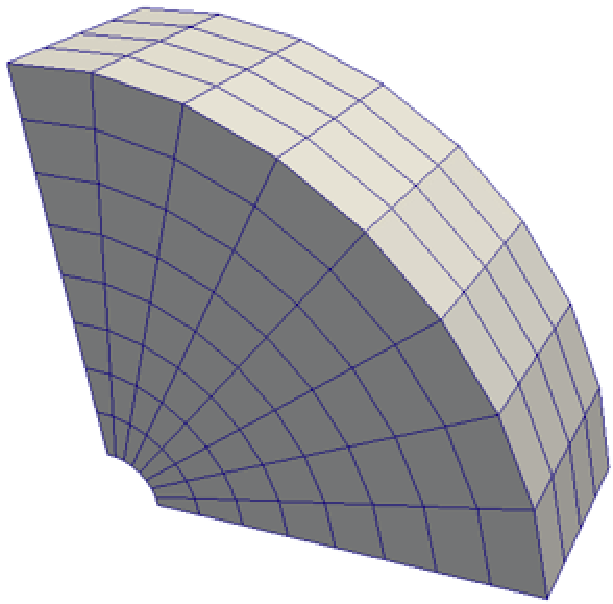
\includegraphics[width=\textwidth]{images/Grids/Curvilinear.pdf}
    \captionsetup{labelformat=empty}
    \caption{\footnotesize Curvilinear}
    \label{fig:Curvilinear}
    \end{figure}
    \tiny
    Curvilinear grids have the same topology as rectilinear grids. However, each point in a curvilinear grid can be placed at an arbitrary coordinate (provided that it does not result in cells that overlap or self intersect).
    \end{column}
    
    \end{columns}
    
\end{frame}{}

\begin{frame}{Poly data and unstructured mesh}

    \begin{columns}[t]
    \begin{column}{0.3\linewidth}
    \begin{figure}
    \centering
    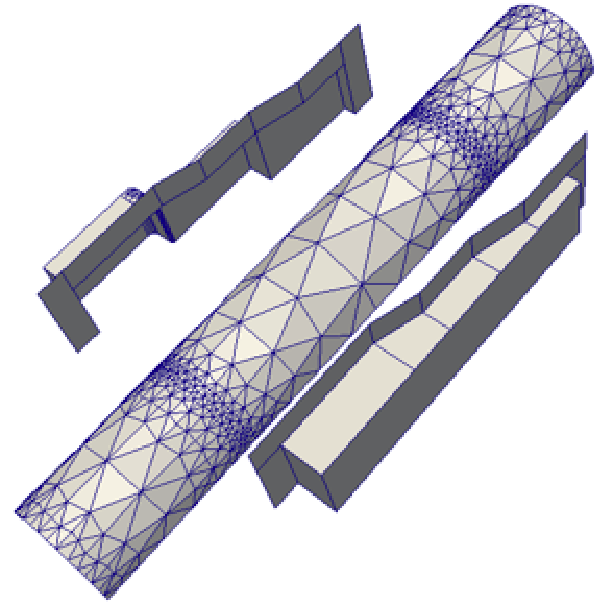
\includegraphics[width=\textwidth]{images/Grids/Polygonal.pdf}
    \captionsetup{labelformat=empty}
    \caption{\footnotesize Polygonal}
    \label{fig:Polygonal}
    \end{figure}
    \tiny
    Polygonal data sets are composed of points, lines, and 2D polygons. Connections between cells can be arbitrary or non-existent.
    
    \end{column}
    
    \begin{column}{0.3\linewidth}
    \begin{figure}
    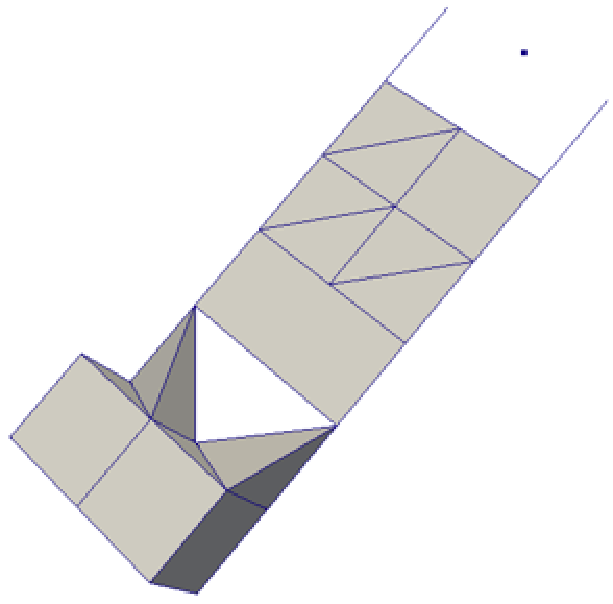
\includegraphics[width=\textwidth]{images/Grids/Unstructured.pdf}
    \captionsetup{labelformat=empty}
    \caption{\footnotesize Unstructured}
    \label{fig:Unstructured}
    \end{figure}
    \tiny
    Unstructured data sets are composed of points, lines, 2D polygons, 3D tetrahedra, and nonlinear cells.
    \end{column}

    \begin{column}{0.3\linewidth}
    \footnotesize
    Also:
    \begin{itemize}
        \item multi-block data
        \item adaptive mesh refinement
        \item ...
    \end{itemize}{}
    
    \tiny Multiblock familiarisation exercise \href{https://www.paraview.org/Wiki/Advanced_Multiblock}{\bf\ul here} for:
    \begin{itemize}
        \item[] \tiny \texttt{Testing/Data/bake/bake.e}
        \item[] \tiny \texttt{Testing/Data/can.ex2}
    \end{itemize}{}
    
    \end{column}
    
    \end{columns}
    
\end{frame}    




\begin{frame}{Data filtering}
Data filtering is the process of choosing a smaller part of your data set and using that subset for viewing or analysis. Filtering is generally (but not always) temporary – the complete data set is kept, but only part of it is used for the calculation

\vskip 12pt

For scientific visualisation, filtering may be used to
\begin{itemize}
    \item Look at results for a particular period of time
    \item Calculate results for particular zone of interest
    \item Present results in an easily understandable manner
    \item Extract important and practically useful measurements
\end{itemize}{}
ParaView has 183 filters listed \href{https://www.paraview.org/Wiki/ParaView/Users_Guide/List_of_filters}{\underline{here}}
\end{frame}{}

\begin{frame}{ParaView data import}
    
    There are two ways to get data into ParaView:
    \begin{itemize}
        \item read data from a file, or
        \item generate data with a source object.
    \end{itemize}{}
    
    \vskip 12pt
    
    ParaView currently supports about 220 distinct file formats
    
\end{frame}{}

\begin{frame}{Exercises: Day 1}
    For Exercise 2.7 in \href{https://docs.paraview.org/en/latest/Tutorials/SelfDirectedTutorial/basicUsage.html#loading-data}{\underline{Section 2.5}}  of the ParaView tutorial, load \texttt{disk\_out\_ref.ex2} from \texttt{ParaView-v5.8.0-RC1/Testing/Data/}
    \begin{itemize}
        \item Stop before Section 2.11
        \item Explore all the different options as you go along
        \item If you finish, create document with image output
    \end{itemize}

    
    
\end{frame}

\section{Data files}

\begin{frame}{Day 2: Understanding data}
    
    Chapter 3 of ParaViewGuide-5.8.0.pdf
    
    \vskip 6pt
    
    VTK data model is used by ParaView
    
    \vskip 6pt
    
    Most fundamental data structure in VTK is a data object
    
    \vskip 6pt
    
    These are either:
    \begin{itemize}
        \item scientific datasets, such as rectilinear grids or finite elements meshes
        \item more abstract data structures, such as graphs or trees
    \end{itemize}{}
    
\end{frame}{}

\begin{frame}{Mesh}
    
    \begin{columns}[t]
    \begin{column}{0.5\linewidth}

    
    Mesh consists of
    \begin{itemize}
        \item Verticies (points)
        \item Cells (elements, zones)
    \end{itemize}{}
    
    \vskip 6pt
    
    Cells are used to discretize a region and can be tetrahedra, hexahedra, etc
    
    \vskip 6pt

    Mapping from cells to vertices is called connectivity
    
    \vskip 6pt
    
    Faces \& edges not represented explicitly by VTK (only needed for arbitrary polyhedron)
    
    \end{column}
    \begin{column}{0.5\linewidth}
    
    \begin{figure}
    \centering
    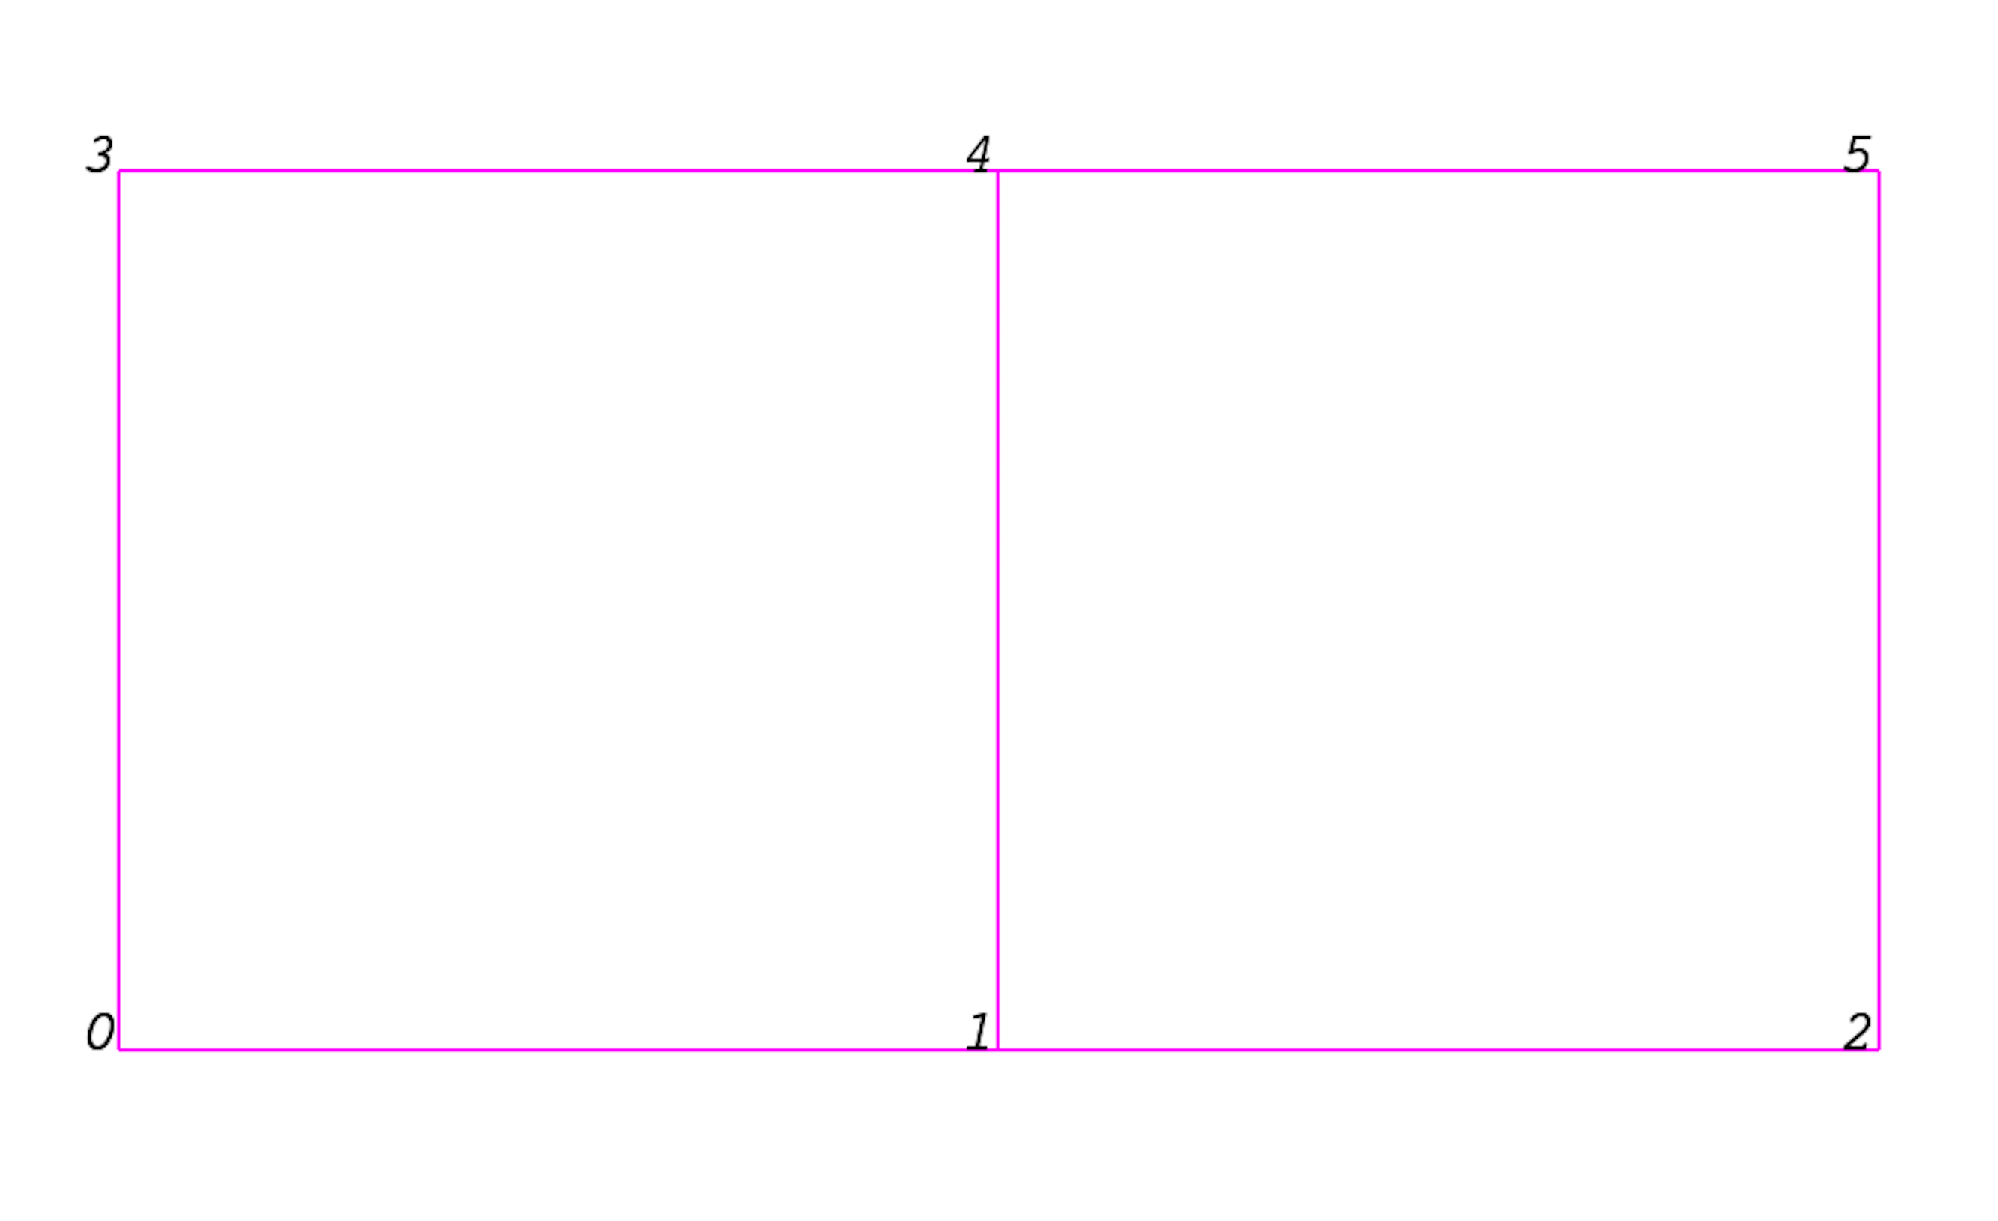
\includegraphics[width=\textwidth]{images/ParaView_UG_Cells.pdf}
    \captionsetup{labelformat=empty}
    \caption{\footnotesize Example of a mesh}
    \label{fig:ParaView_UG_Cells}
    \end{figure}
    
    \begin{itemize}
        \item Cell 1; 0, 1, 3, 4
        \item Cell 2; 1, 2, 4, 5
    \end{itemize}{}
    Share points 1 & 4
    
    
    \end{column}
    \end{columns}
    
\end{frame}{}

\begin{frame}{Attributes (fields, arrays)}
    
    Data attributes stored at different mesh locations
    \begin{itemize}
        \item May depend on calculation, e.g. velocity at vertices and cell centred pressure
    \end{itemize}{}
    
    \vskip -12pt
    
    \begin{columns}[t]
    \begin{column}{0.5\linewidth}
    \begin{figure}
    \centering
    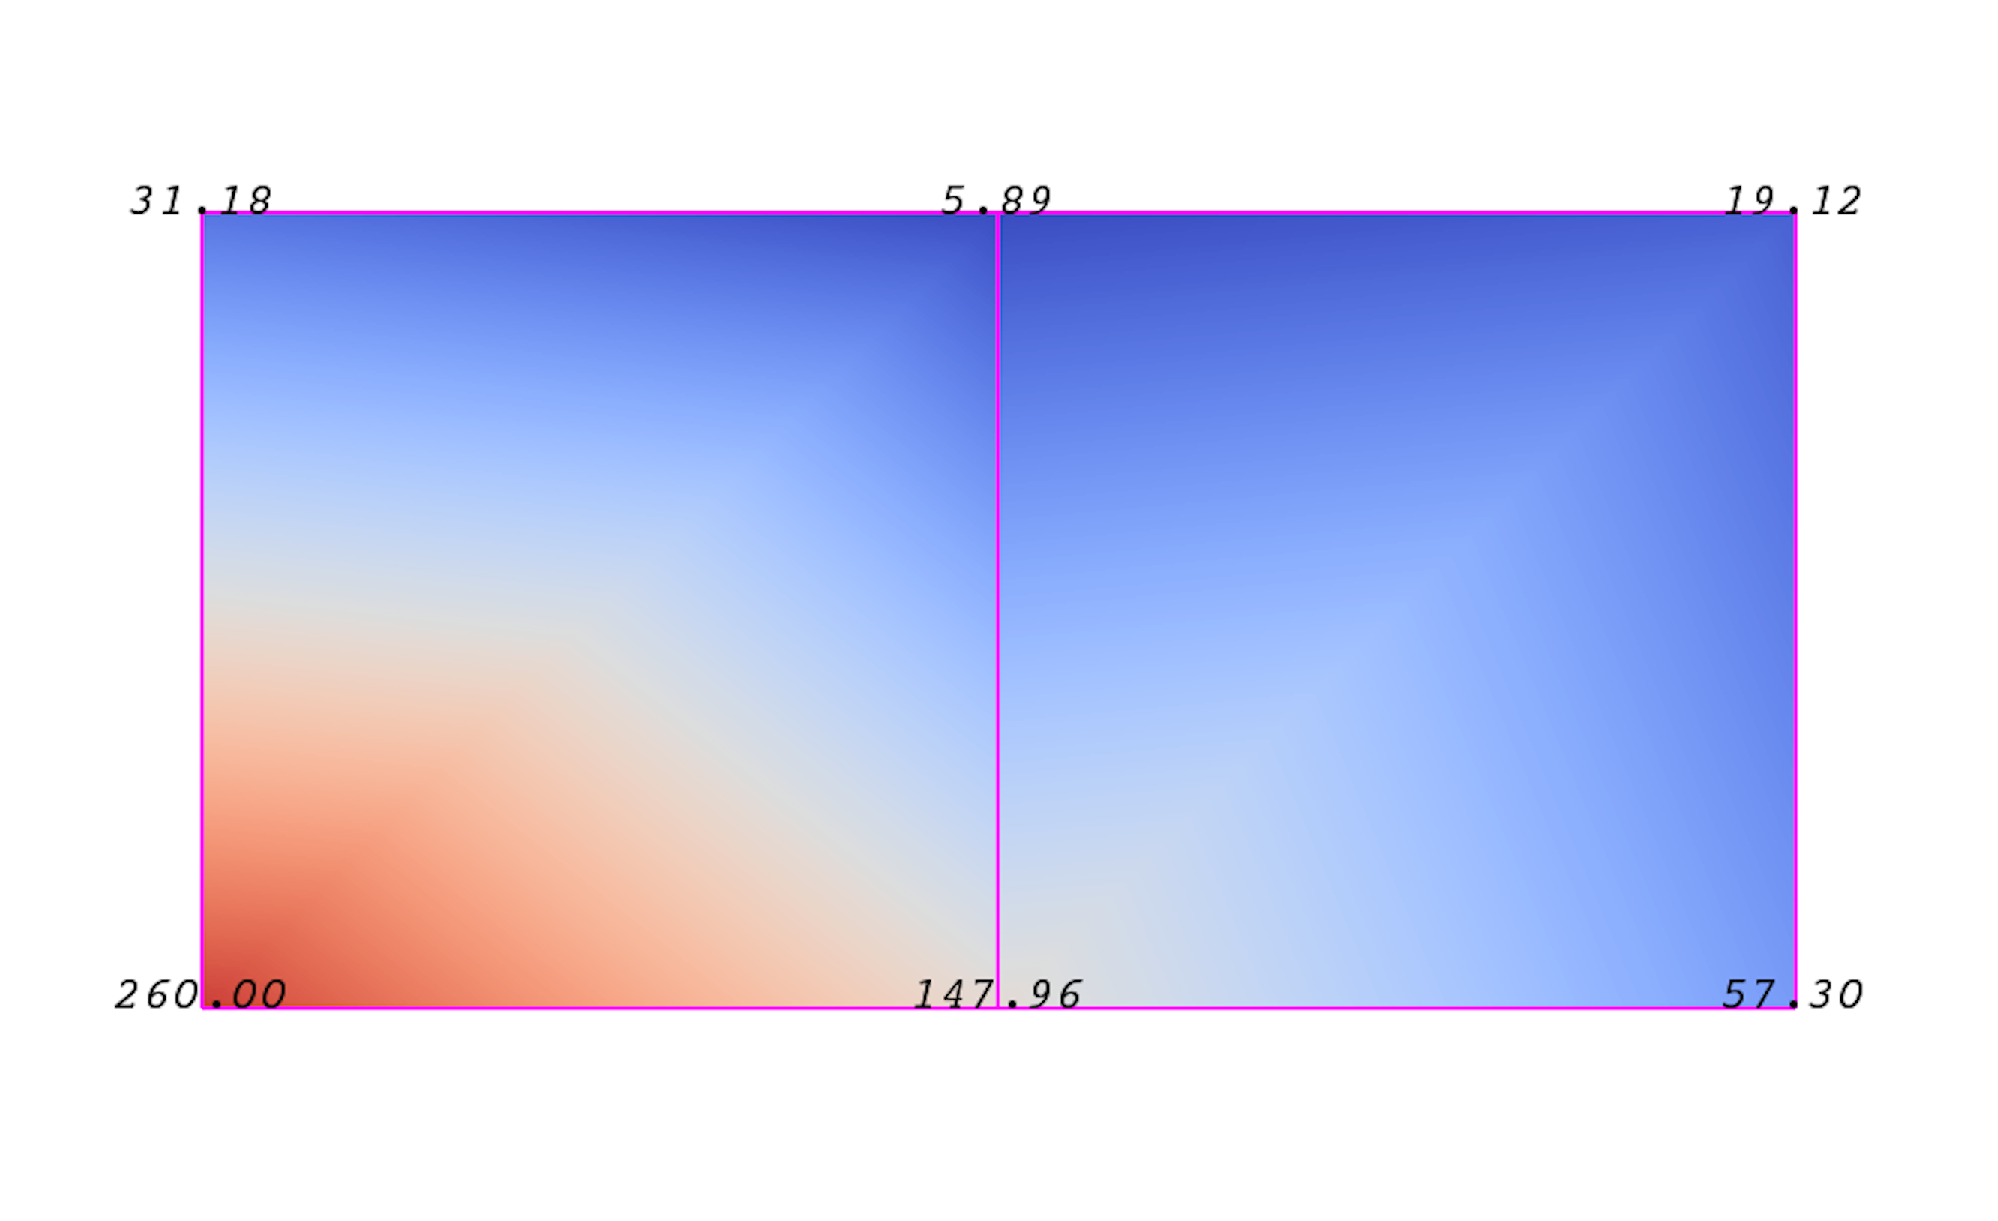
\includegraphics[width=\textwidth]{images/ParaView_UG_Cells_with_values.pdf}
    \captionsetup{labelformat=empty}
    \caption{\footnotesize Point-centered attribute in a data array or field}
    \label{fig:ParaView_UG_Cells_with_values}
    \end{figure}
    
    \footnotesize
    \vskip -12pt
    
    Attribute only defined at vertices
    \begin{itemize}
        \item Interpolation used to obtain values everywhere else
    \end{itemize}{}
    
    
    \end{column}
    \begin{column}{0.5\linewidth}
    \begin{figure}
    \centering
    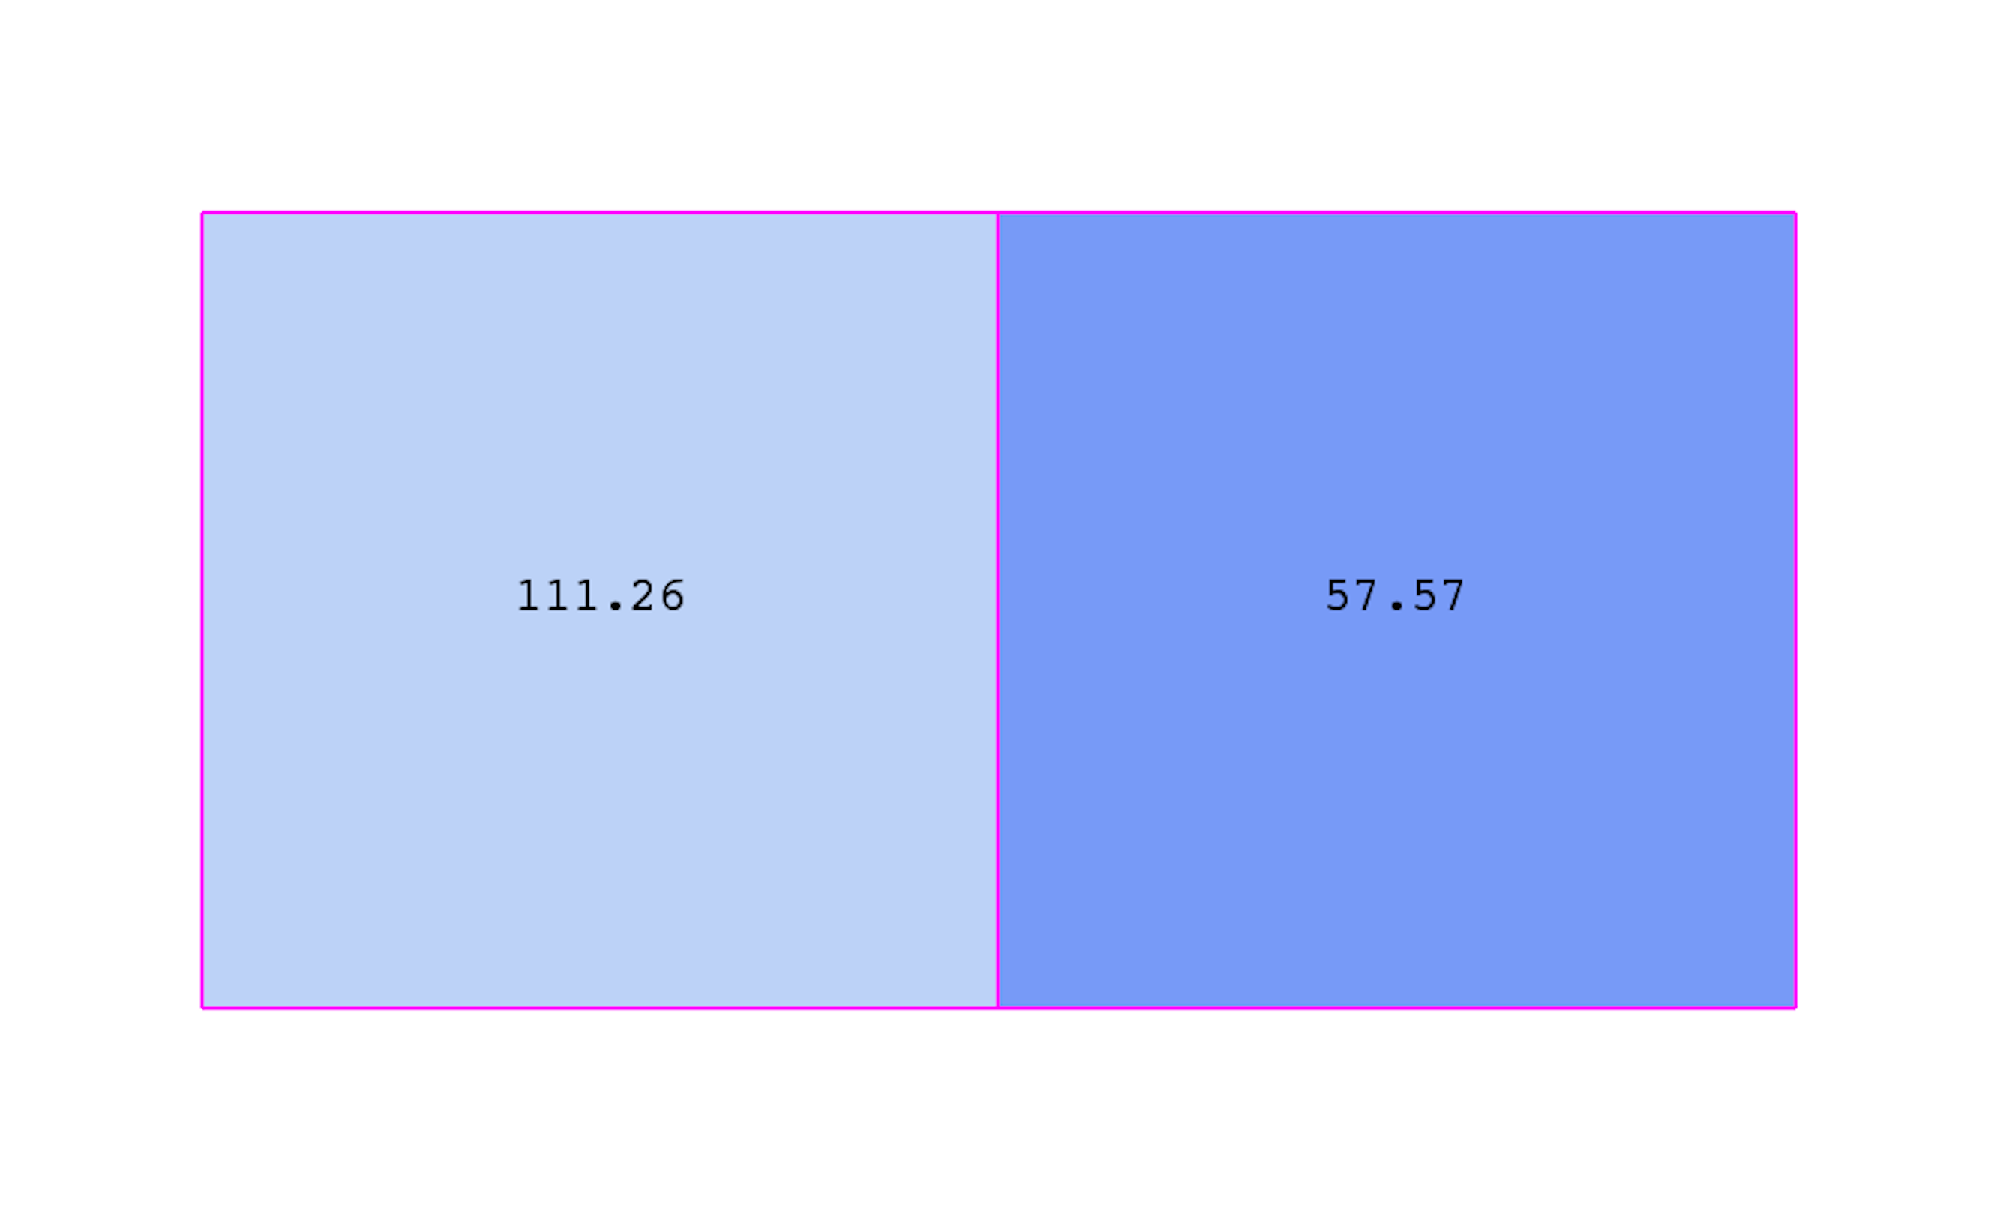
\includegraphics[width=\textwidth]{images/ParaView_UG_Cells_with_cvalues.pdf}
    \captionsetup{labelformat=empty}
    \caption{\footnotesize Cell-centred attribute}
    \label{fig:ParaView_UG_Cells_with_cvalues}
    \end{figure}
    \footnotesize
    
    \vskip -12pt
    
    Cell-centered attributes are assumed to be constant over each cell
    \begin{itemize}
        \item Filter may not apply; requires \texttt{Cell Data to
Point Data} filter
    \end{itemize}{}
    
    \end{column}
    
    
    \end{columns}
    
\end{frame}{}

\begin{frame}{VTK Data file formats}
    
    VTK supports five different data-set formats:
    \begin{itemize}
        \item structured points, structured grid, rectilinear grid, unstructured grid, polygonal data
    \end{itemize}{}
    
    \vskip 6pt
    
    \begin{columns}[t]
    \begin{column}{0.5\linewidth}
    Exercise; Create \texttt{file1.vtk}:
    
    \vskip 6pt
    
    \footnotesize
    \texttt{\# vtk DataFile Version 2.0}\newline
    \texttt{Structured example}\newline
    \texttt{ASCII}\newline
    \texttt{DATASET STRUCTURED\_POINTS}\newline
    \texttt{DIMENSIONS 3 4 5}\newline
    \texttt{ORIGIN 0 0 0}\newline
    \texttt{SPACING 1 2 3}\newline
    
    Now open with ParaView (beware! `\_' character doesn't copy-paste)
    \end{column}
    
    \begin{column}{0.5\linewidth}
    Then add lines:
    \vskip 6pt
    
    \footnotesize
    \texttt{POINT\_DATA 60}\newline
    \texttt{SCALARS volume\_scalars char 1}\newline
    \texttt{LOOKUP\_TABLE default}\newline
    {\tiny
    \texttt{0 0 0 0 0 0 0 0 0 0 0 0}\newline
    \texttt{0 5 10 15 20 25 25 20 15 10 5 0}\newline
    \texttt{0 10 20 30 40 50 50 40 30 20 10 0}\newline
    \texttt{0 5 10 15 20 25 25 20 15 10 5 0}\newline
    \texttt{0 0 0 0 0 0 0 0 0 0 0 0}\newline
    }
    
    Open in ParaView and check data.

    \vskip 6pt

    Can you add cell data?
    
    
    \end{column}
    \end{columns}

\end{frame}{}

\begin{frame}{Unstructured grid example}

    \begin{columns}[t]
    \begin{column}{0.5\linewidth}

    \tiny
    \vskip -13pt
    \texttt{\# vtk DataFile Version 2.0}\newline
\texttt{Unstructured Ex}\newline
\texttt{ASCII}\newline
\texttt{DATASET UNSTRUCTURED\_GRID}\newline
\texttt{POINTS 27 float}\newline
\texttt{0 0 0  1 0 0  2 0 0  0 1 0  1 1 0  2 1 0  0 0 1}\newline
\texttt{1 0 1  2 0 1  0 1 1  1 1 1  2 1 1  0 1 2  1 1 2}\newline
\texttt{2 1 2  0 1 3  1 1 3  2 1 3  0 1 4  1 1 4  2 1 4}\newline
\texttt{0 1 5  1 1 5  2 1 5  0 1 6  1 1 6  2 1 6}\newline
\texttt{CELLS 11 60}\newline
\texttt{8 0 1 4 3 6 7 10 9}\newline
\texttt{8 1 2 5 4 7 8 11 10}\newline
\texttt{4 6 10 9 12}\newline
\texttt{4 5 11 10 14}\newline
\texttt{6 15 16 17 14 13 12}\newline
\texttt{6 18 15 19 16 20 17}\newline
\texttt{4 22 23 20 19}\newline
\texttt{3 21 22 18}\newline
\texttt{3 22 19 18}\newline
\texttt{2 26 25}\newline
\texttt{1 24}\newline
\texttt{CELL\_TYPES 11}\newline
\texttt{12 12 10 10 7 6 9 5 5 3 1}\newline
\texttt{POINT\_DATA 27}\newline
\texttt{SCALARS scalars float 1}\newline
\texttt{LOOKUP\_TABLE default}\newline
\texttt{0.0 1.0 2.0 3.0 4.0 5.0 6.0}\newline
\texttt{7.0 8.0 9.0 10.0 11.0 12.0}\newline
\texttt{13.0 14.0 15.0 16.0 17.0 18.0}\newline
\texttt{19.0 20.0 21.0 22.0 23.0 24.0 25.0 26.0}\newline
\texttt{VECTORS vectors float}\newline
\texttt{1 0 0  1 1 0  0 2 0  1 0 0  1 1 0  0 2 0  1 0 0}\newline
\texttt{1 1 0  0 2 0  1 0 0  1 1 0  0 2 0  0 0 1  0 0 1}\newline
\texttt{0 0 1  0 0 1  0 0 1  0 0 1  0 0 1  0 0 1  0 0 1}\newline
\texttt{0 0 1  0 0 1  0 0 1  0 0 1  0 0 1  0 0 1}\newline

\end{column}

    \begin{column}{0.5\linewidth}
    
        \begin{figure}
    \centering
    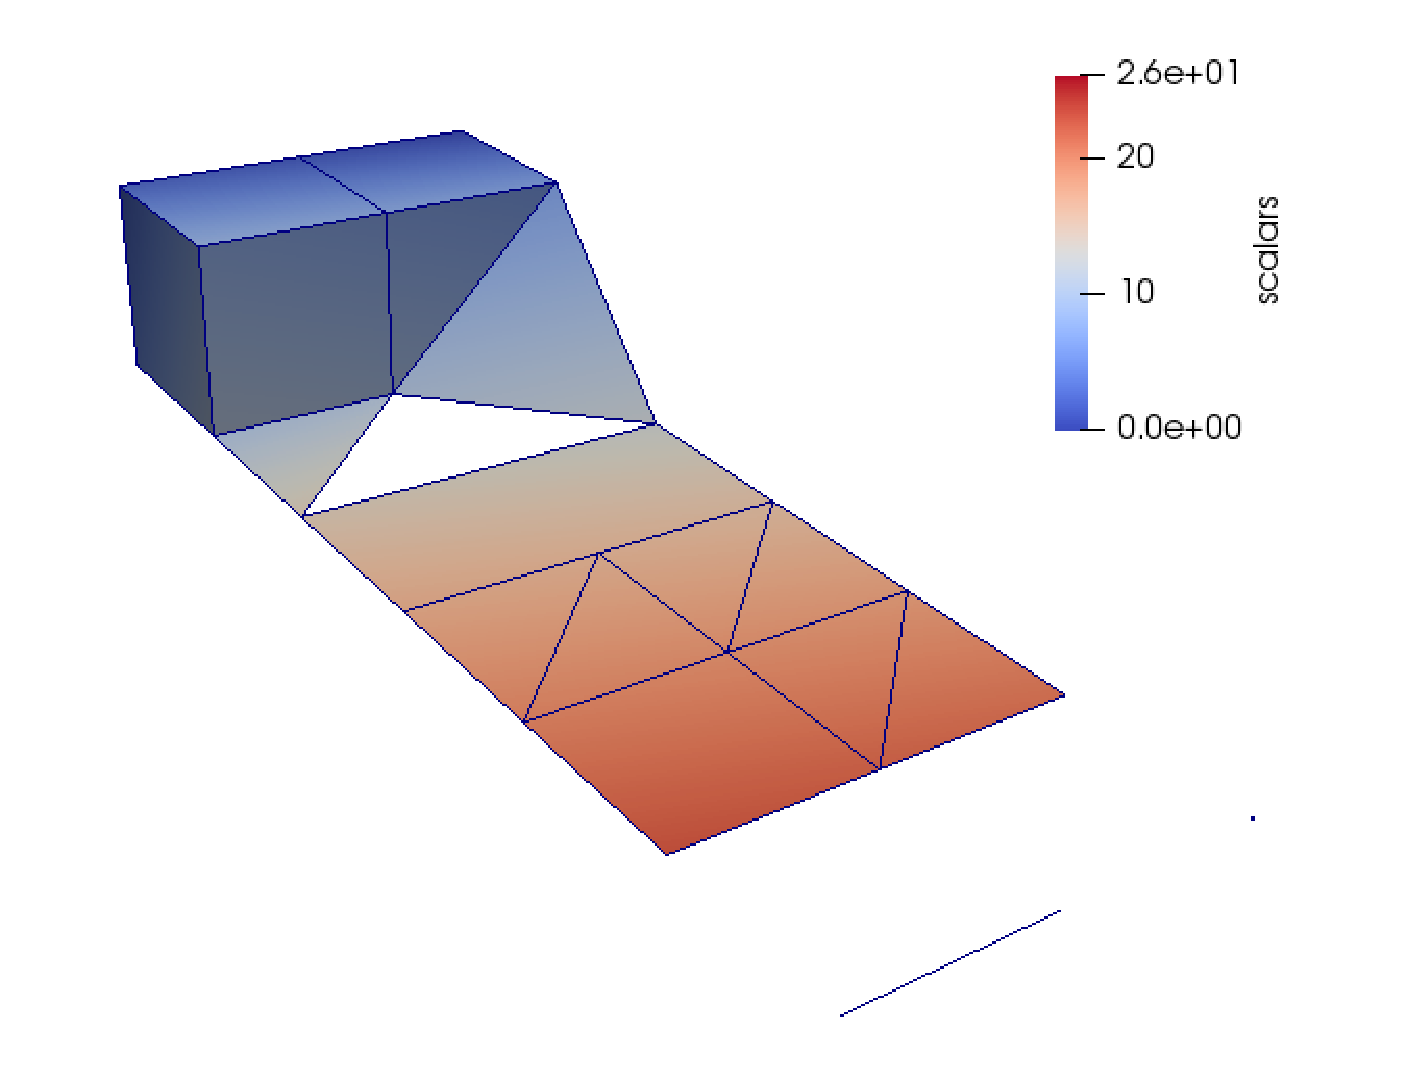
\includegraphics[width=\textwidth]{images/UnstructuredMesh.pdf}
    \captionsetup{labelformat=empty}
    \caption{\footnotesize Mesh given by \texttt{Unstructured Ex} (left)}
    \label{fig:UnstructuredMesh}
    \end{figure}
    
    \vskip 12pt
    
    \footnotesize{Details on \texttt{CELL\_TYPES} given \href{https://vtk.org/wp-content/uploads/2015/04/file-formats.pdf}{\bf\underline{here}} on pp. 9 \& 10}
    
    \end{column}

\end{columns}

\end{frame}{}

\begin{frame}{Time dependent data}
    
    ParaView automatically detects several file naming patterns that indicate a file series, including:

\vskip 6pt
\small{\centering
\texttt{fooN.vtk} \qquad
\texttt{foo\_N.vtk} \qquad
\texttt{foo\-N.vtk} \qquad
\texttt{foo.N.vtk} \qquad
\texttt{Nfoo.vtk} \qquad
\texttt{N.foo.vtk} \qquad
\texttt{foo.vtk.N} \qquad
\texttt{foo.vtk\-sN} \qquad
}
\vskip 6pt

where \emph{foo} is any filename, \emph{N} is a numeral sequence, and \emph{vtk} could be any extension
    
\vskip 6pt

    File sequences can be made that will be grouped by ParaView; e.g. \texttt{file1.vtk}, \texttt{file2.vtk}, ...
    
\end{frame}{}

\begin{frame}{Particle file 1}
    
    \footnotesize
    Create file named \texttt{part0.vtu} with:
    
    \tiny
    \vskip 6pt
    
    \texttt{<VTKFile type="UnstructuredGrid" version="2.0" byte\_order="LittleEndian">}\newline
\texttt{  <UnstructuredGrid>}\newline
\texttt{    <Piece NumberOfPoints="3" NumberOfCells="0">}\newline
\texttt{      <Points>}\newline
\texttt{        <DataArray name="Position" type="Float32" NumberOfComponents="3" format="ascii">}\newline
\texttt{          0 0 0 1 1 1 0 0 1}\newline
\texttt{        </DataArray>}\newline
\texttt{      </Points>}\newline
\texttt{      <PointData  Vectors="vector">}\newline
\texttt{        <DataArray type="Float32" Name="Velocity" NumberOfComponents="3" format="ascii">}\newline
\texttt{          4 4 4 4 0 0 2 2 -2}\newline
\texttt{        </DataArray>}\newline
\texttt{        <DataArray type="Float32" Name="Diameter" format="ascii">}\newline
\texttt{          0.1 0.5 1}\newline
\texttt{        </DataArray>}\newline
\texttt{        <DataArray type="Float32" Name="Temperature" format="ascii">}\newline
\texttt{          273 300 350}\newline
\texttt{        </DataArray>}\newline
\texttt{      </PointData>}\newline
\texttt{      <Cells>}\newline
\texttt{        <DataArray type="Int32" Name="connectivity" format="ascii">}\newline
\texttt{        </DataArray>}\newline
\texttt{        <DataArray type="Int32" Name="offsets" format="ascii">}\newline
\texttt{        </DataArray>}\newline
\texttt{        <DataArray type="UInt8" Name="types" format="ascii">}\newline
\texttt{        </DataArray>}\newline
\texttt{      </Cells>}\newline
\texttt{    </Piece>}\newline
\texttt{  </UnstructuredGrid>}\newline
\texttt{</VTKFile>}\newline

\end{frame}{}

\begin{frame}{Particle file 2}
    
    \begin{columns}[t]
    \begin{column}{0.5\linewidth}

    \begin{itemize}
        \item Open file in ParaView
        \item Add glyphs with diameter specified in file (change Properties$\rightarrow$Glyph Mode to All Points)
        \item Colour particles according to temperature
        \item Copy \texttt{part0.vtu} to create \texttt{part1.vtu} with different particle coordinates/temperature/diameter
    \end{itemize}{}
    
    \end{column}
    \begin{column}{0.5\linewidth}
    
    \begin{figure}
    \centering
    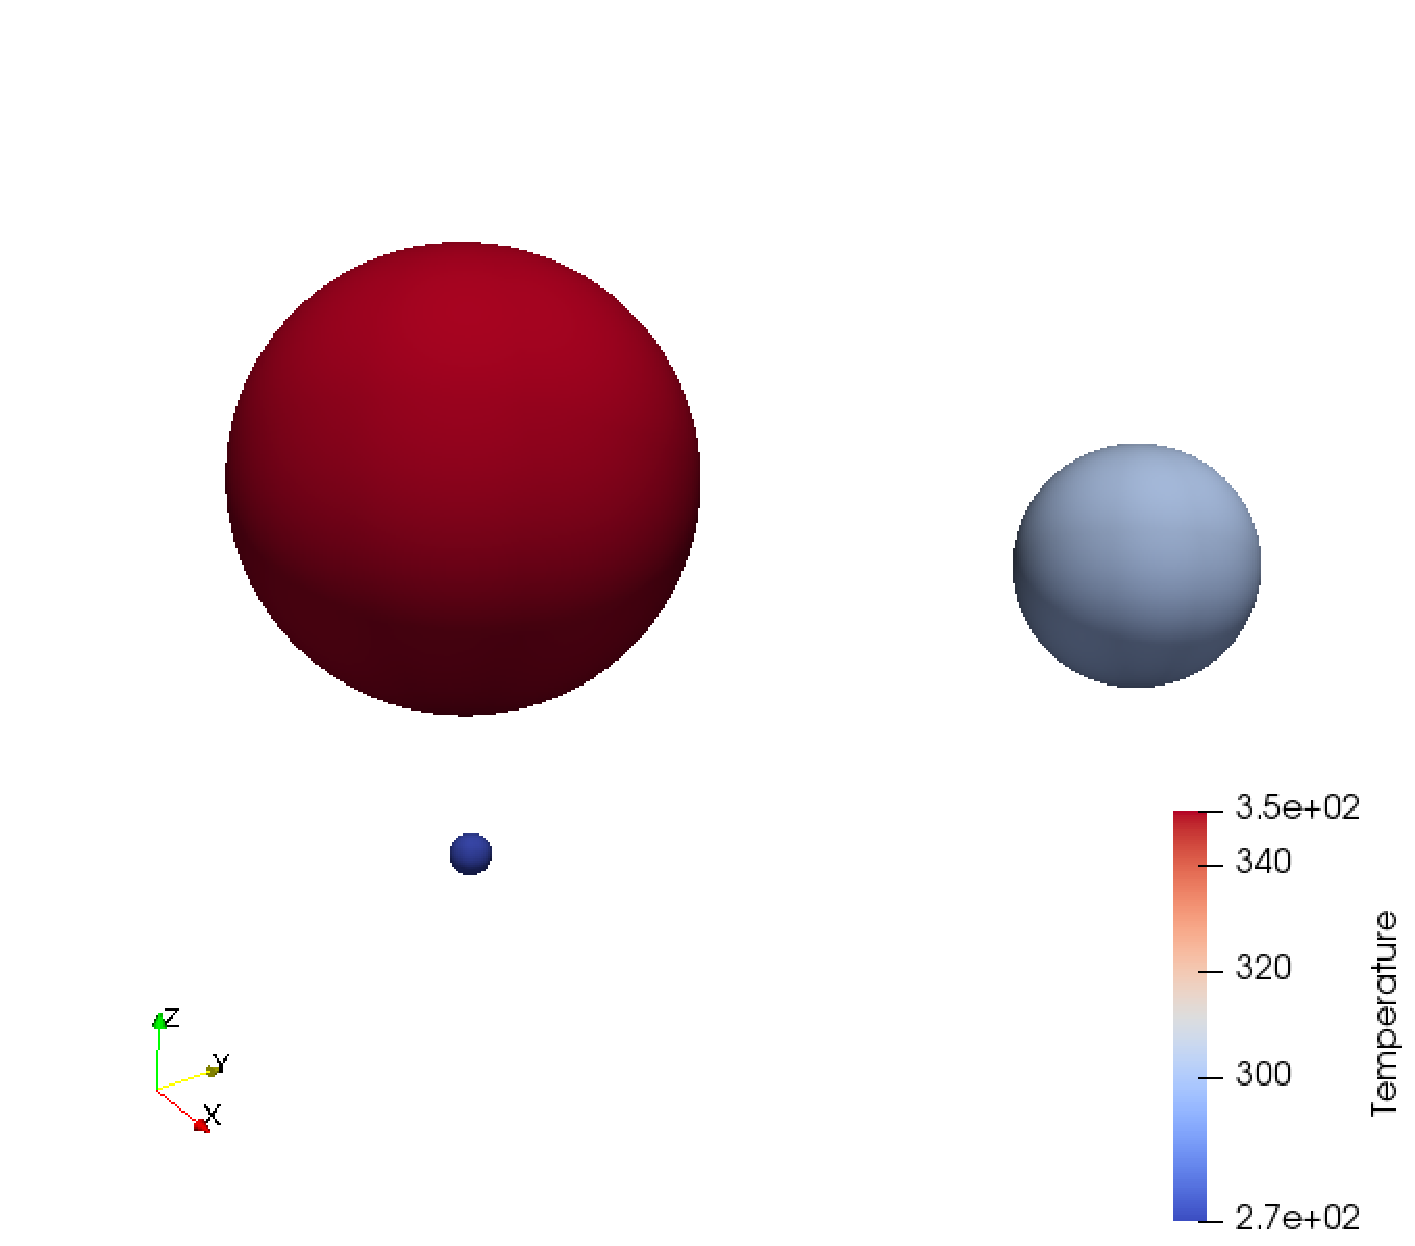
\includegraphics[width=\textwidth]{images/particles.pdf}
    \captionsetup{labelformat=empty}
    \caption{\footnotesize Particles}
    \label{fig:particles}
    \end{figure}
    
    \end{column}
    \end{columns}
    
\end{frame}{}

\begin{frame}{Other file formats}
    
    \href{https://en.wikipedia.org/wiki/STL_(file_format)}{\bf\underline{STL}} ("stereolithography") file, e.g. \href{https://commons.wikimedia.org/wiki/File:Utah_teapot_(solid).stl}{\bf\underline{Utah teapot}}
    \begin{itemize}
        \item Describe only the surface geometry of a three-dimensional object
        \item Unstructured triangulated surface
    \end{itemize}{}
    
    \vskip 6pt
    
    \href{https://cubit.sandia.gov/public/13.2/help_manual/WebHelp/finite_element_model/exodus/block_specification.htm}{\bf\underline{Exodus}} Element Block Specification (e.g. \texttt{.ex2})
    \begin{itemize}
        \item \href{https://cubit.sandia.gov/}{\bf\underline{CUBIT}} Geometry and Mesh Generation Toolkit
    \end{itemize}{}
    
    \vskip 6pt
    
    Binary files
    \begin{itemize}
        \item More compact and quicker to read
        \item Binary versions of most file formats
    \end{itemize}{}
    
\end{frame}{}

\begin{frame}{Grid generation: Gmsh}

Normally, a mesh is generated by software

\vskip 6pt

    \begin{columns}[t]
    \begin{column}{0.5\linewidth}
    
    \small

For example, \href{http://gmsh.info/}{\bf\underline{Gmsh}} open-source finite-element mesh generator. After installing Gmsh:
\begin{enumerate}
    \item Download script \href{https://gitlab.onelab.info/gmsh/gmsh/-/blob/master/tutorial/t4.geo}{\bf\underline{t4.geo}}
    \item run command \texttt{\$ gmsh -2 -format stl t4.geo}
    \item open \texttt{t4.stl} in ParaView
\end{enumerate}{}

    \end{column}
    \begin{column}{0.5\linewidth}

\begin{figure}
    \centering
    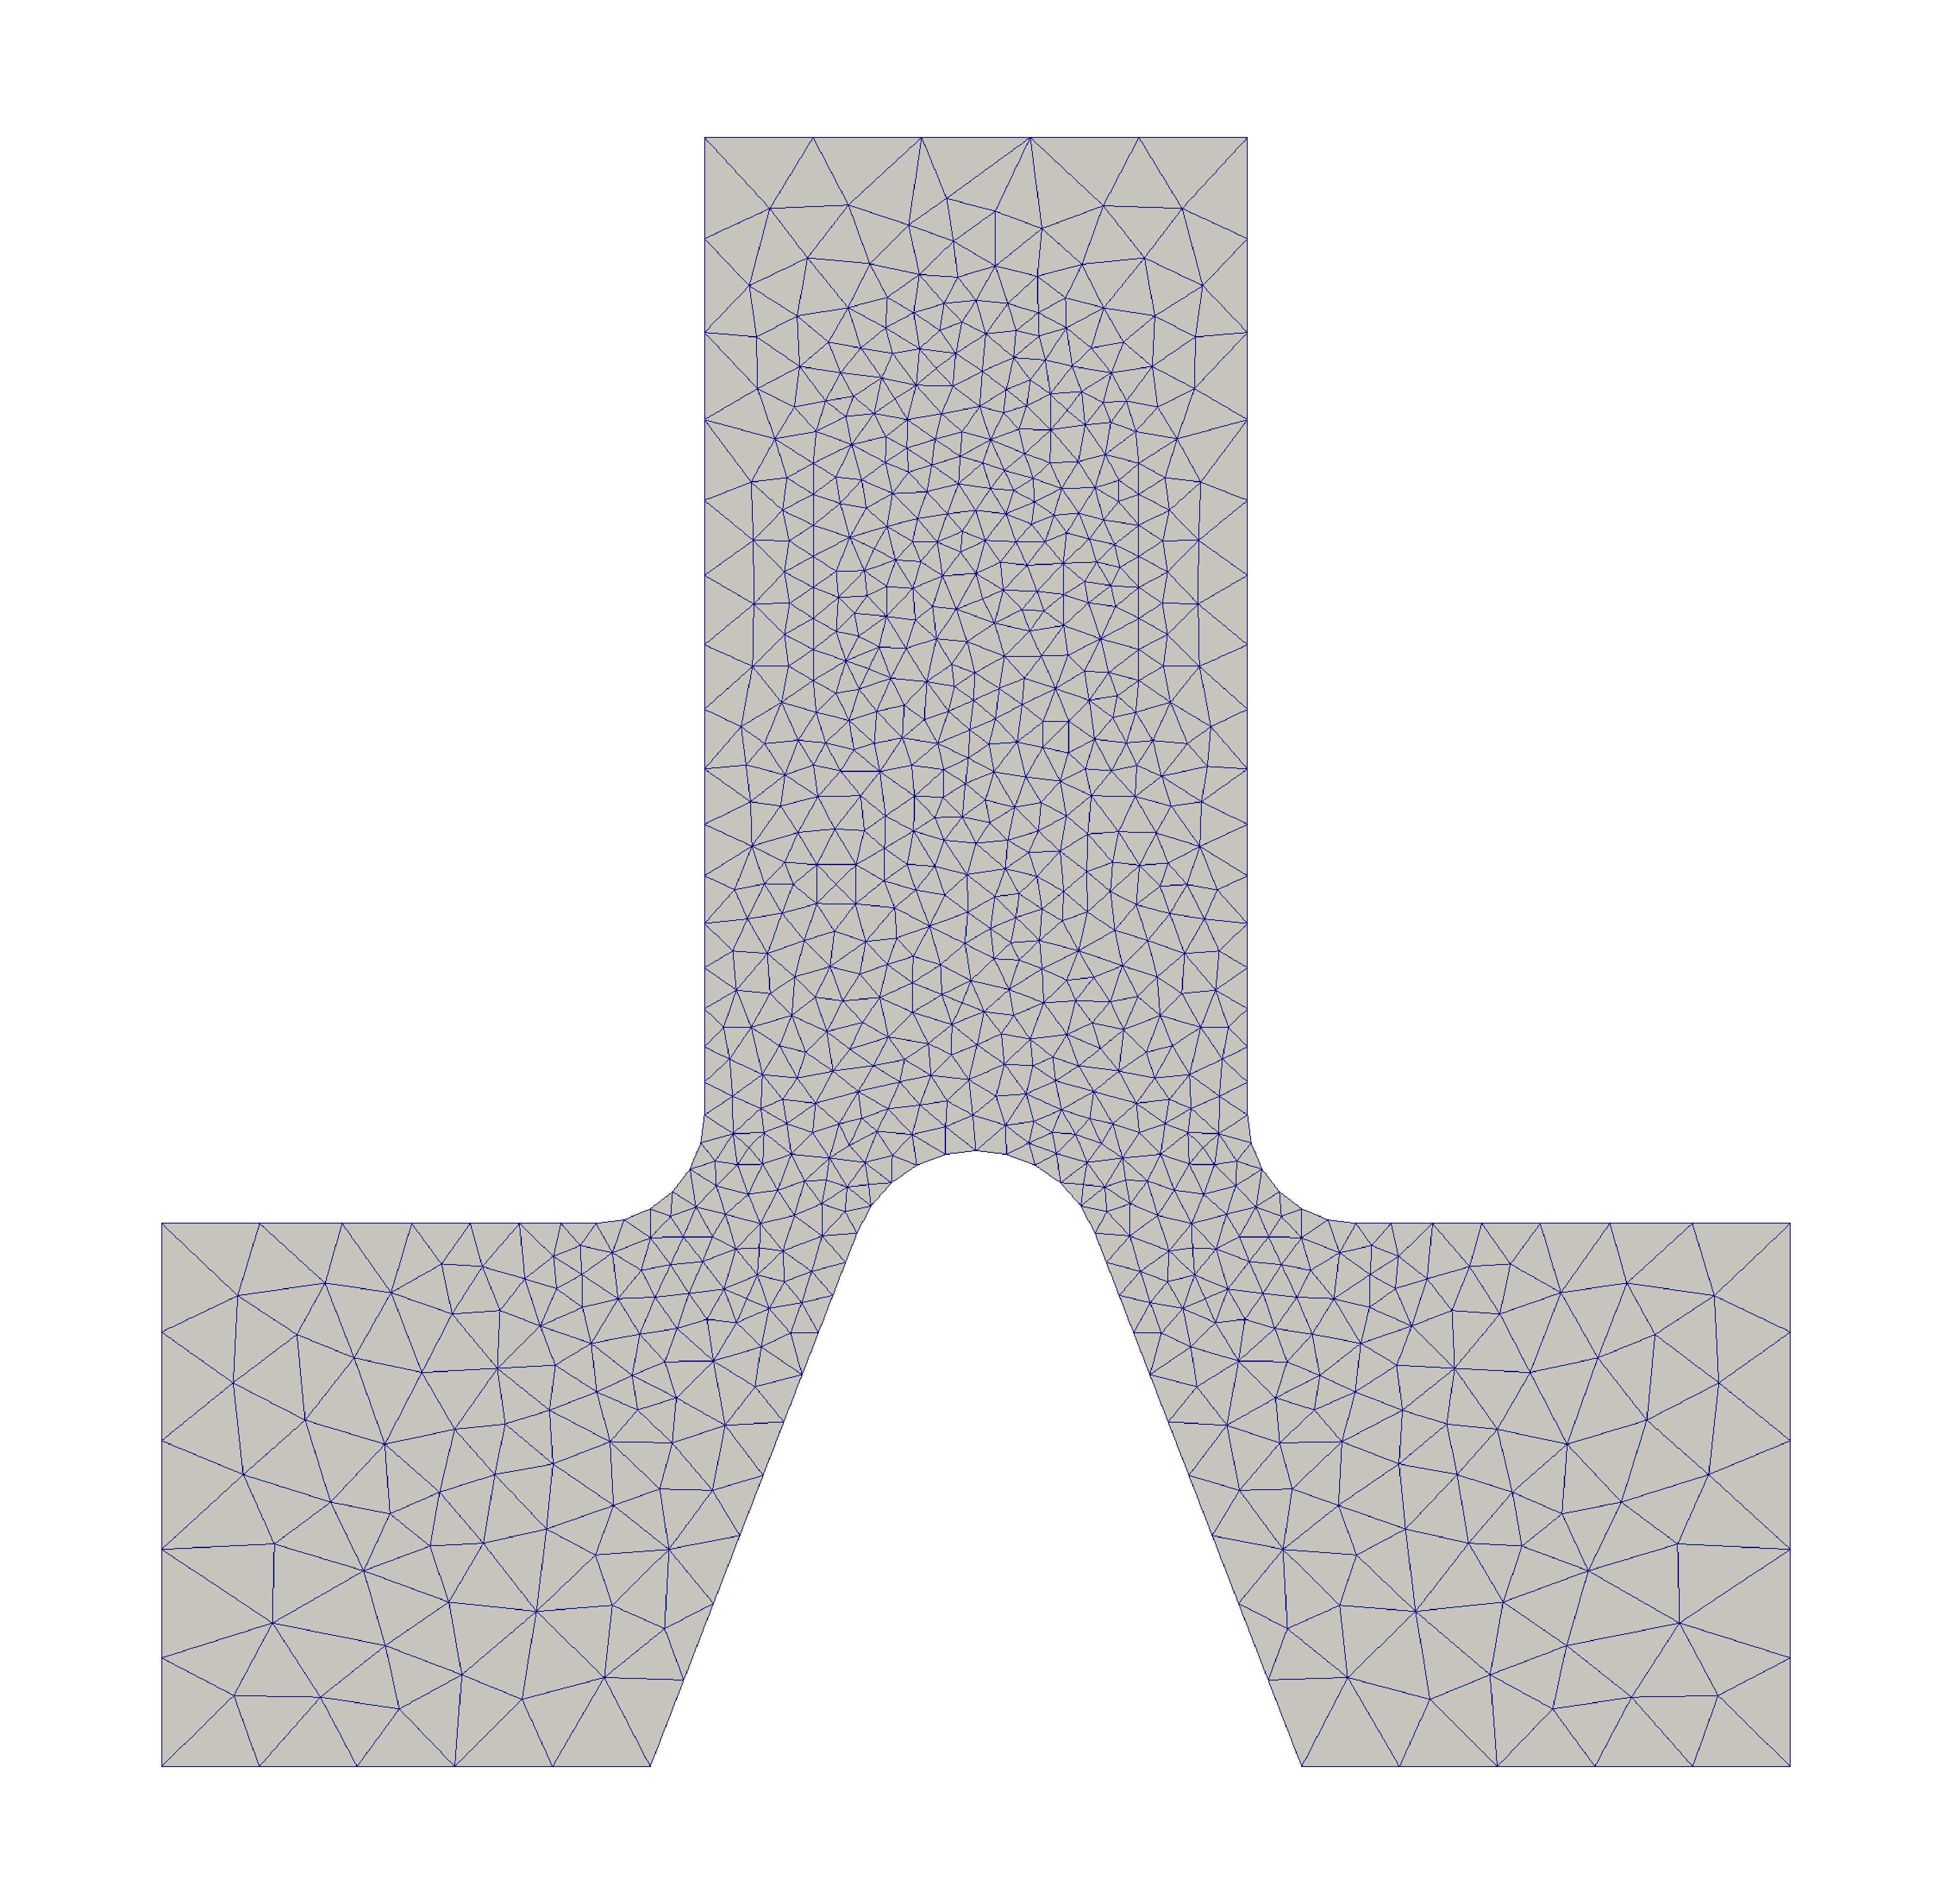
\includegraphics[width=\textwidth]{images/t4_gmsh.pdf}
    \captionsetup{labelformat=empty}
    \caption{\footnotesize Mesh generated with \texttt{Gmsh}}
    \label{fig:t4_gmsh}
    \end{figure}
    
    \end{column}
    \end{columns}
    
\end{frame}{}

%\begin{frame}{Computer simulation}
%  3D data from \href{https://en.wikipedia.org/wiki/Computer_simulation}{\bf\underline{computer simulation}}
%\end{frame}{}

\begin{frame}{Computer simulation: OpenFOAM}

    \begin{columns}[t]
    \begin{column}{0.5\linewidth}
    \href{https://openfoam.org/}{\bf\underline{OpenFOAM}} is free, open source software for CFD
    
    \vskip 6pt
    
    Can be obtained on Ubuntu from \href{https://develop.openfoam.com/Development/openfoam/-/wikis/precompiled/debian}{\underline{here}}
        
    \vskip 6pt
    
    Tutorial examples including cylinder potential flow (right)
    
    \vskip 6pt
    
{\tiny\texttt{\quad \$FOAM\_TUTORIALS/tutorials/basic/potentialFoam/cylinder}}
    
    \vskip 6pt
    
    Version of ParaView launched from command line:
    
    \vskip 6pt
    
    \texttt{\tiny\quad\$ paraFoam}
    
    
    \end{column}

    \begin{column}{0.5\linewidth}
    
    \begin{figure}
    \centering
    \captionsetup{labelformat=empty}
    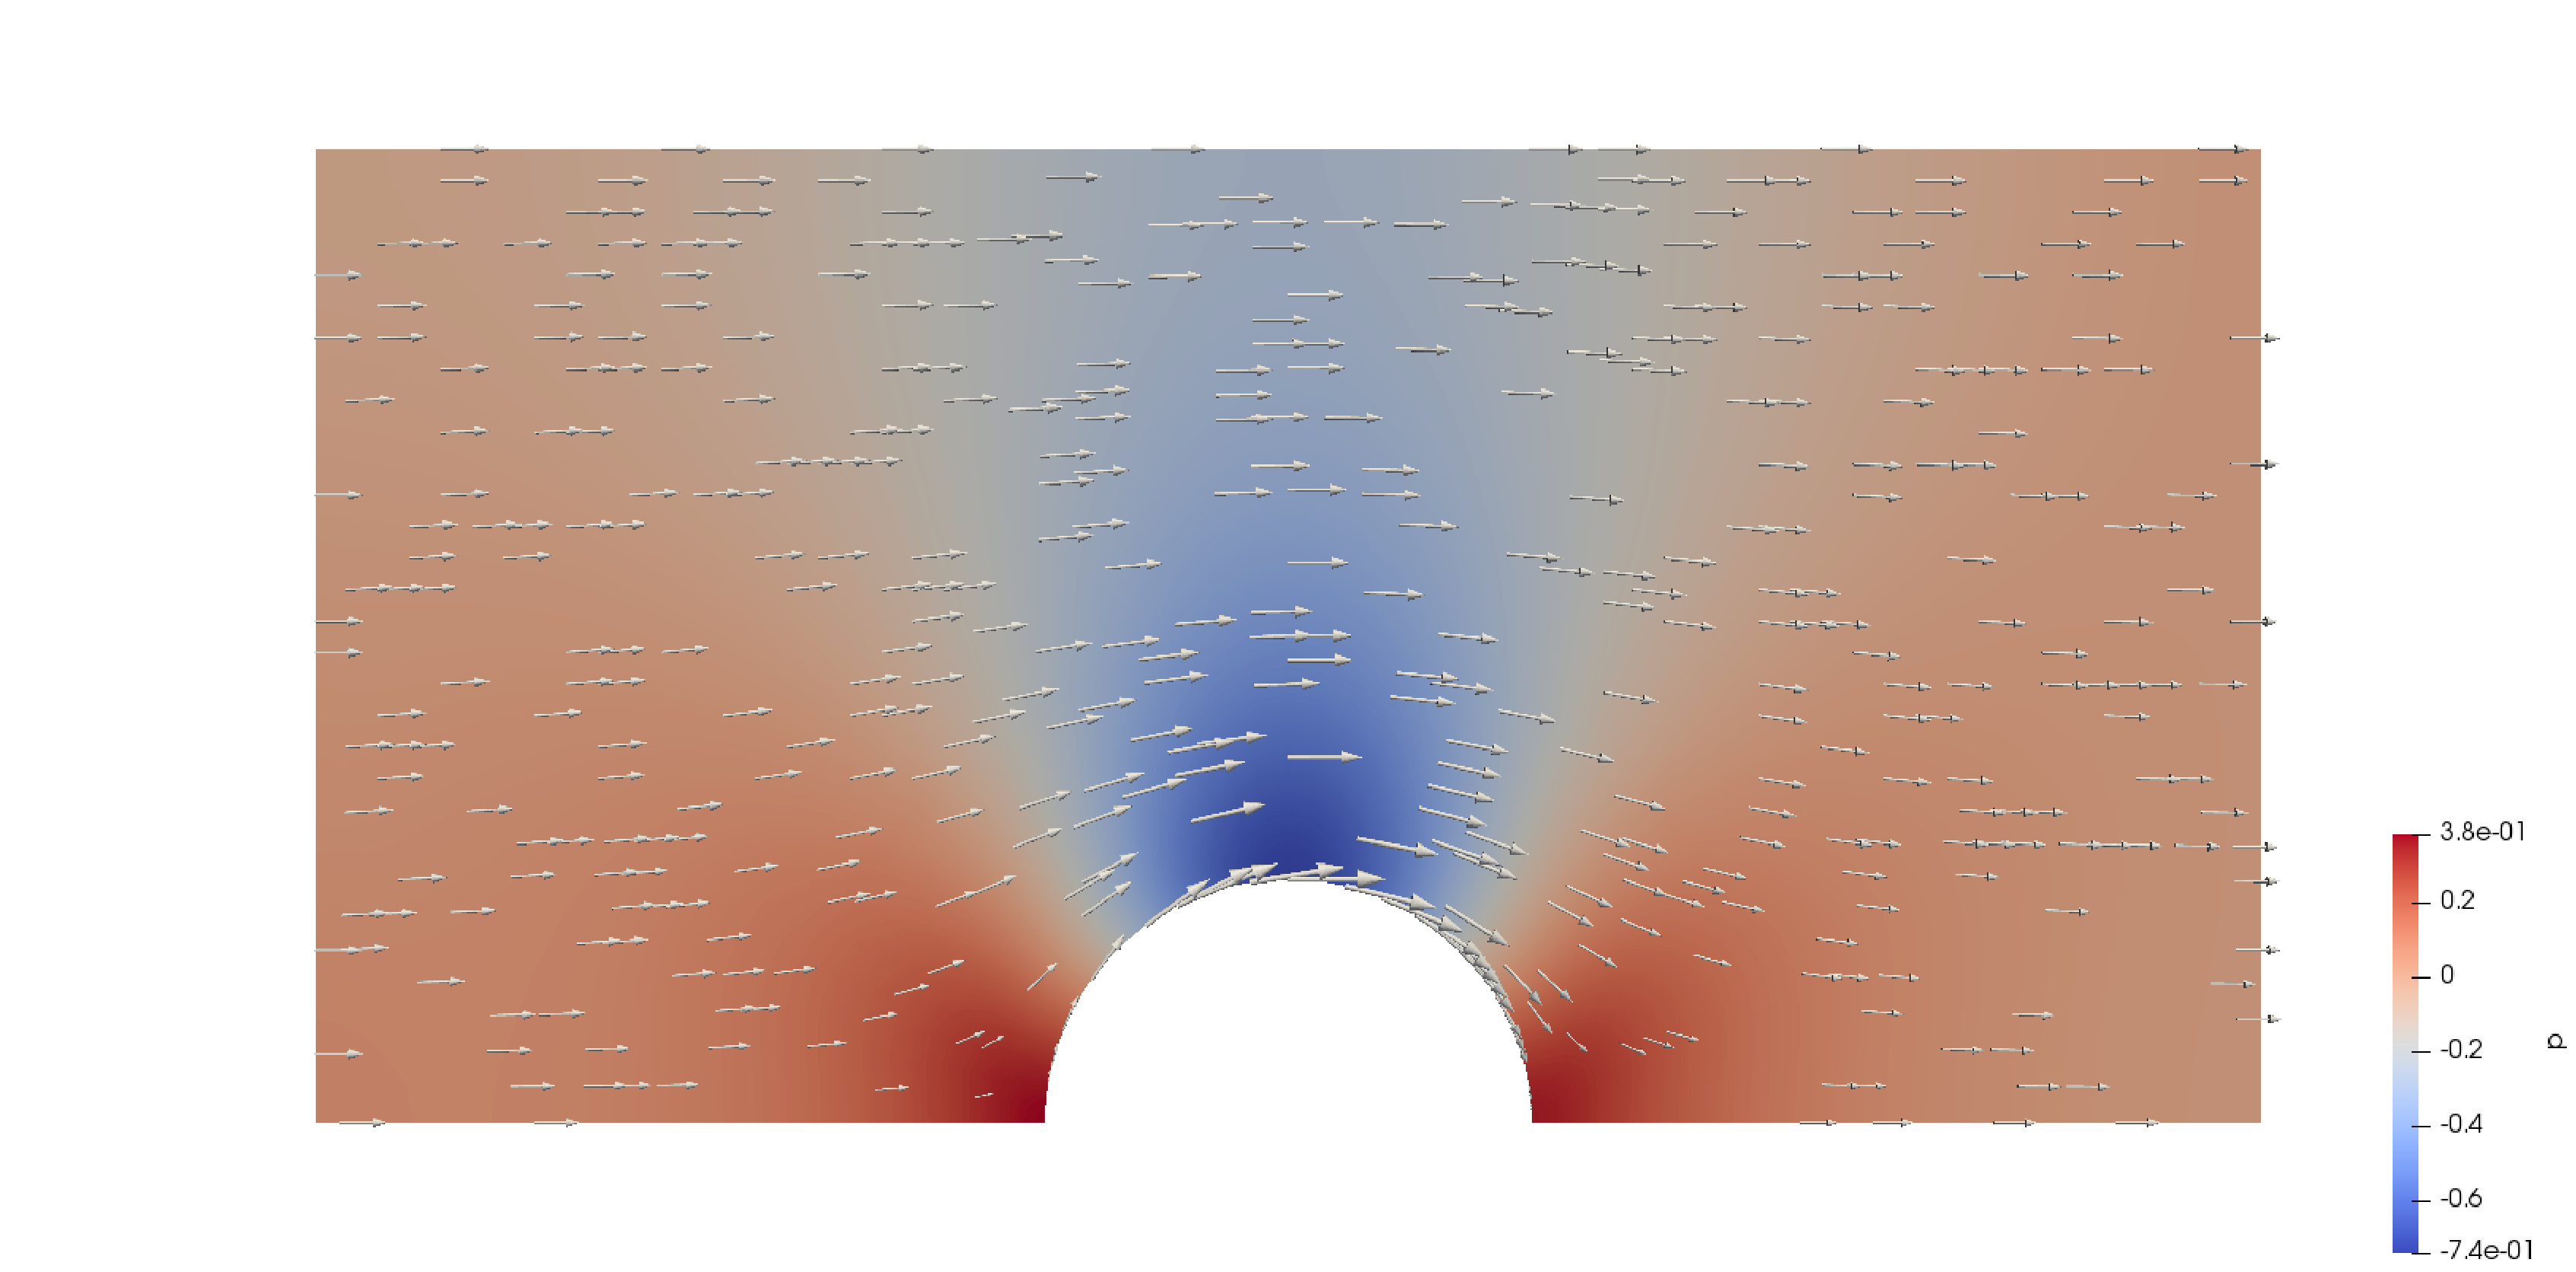
\includegraphics[trim={250 100 250 100},clip, width=\textwidth]{images/Pressure_and_Glyphs.pdf}
    \tiny{Pressure and glyphs}
    \vskip 6pt
    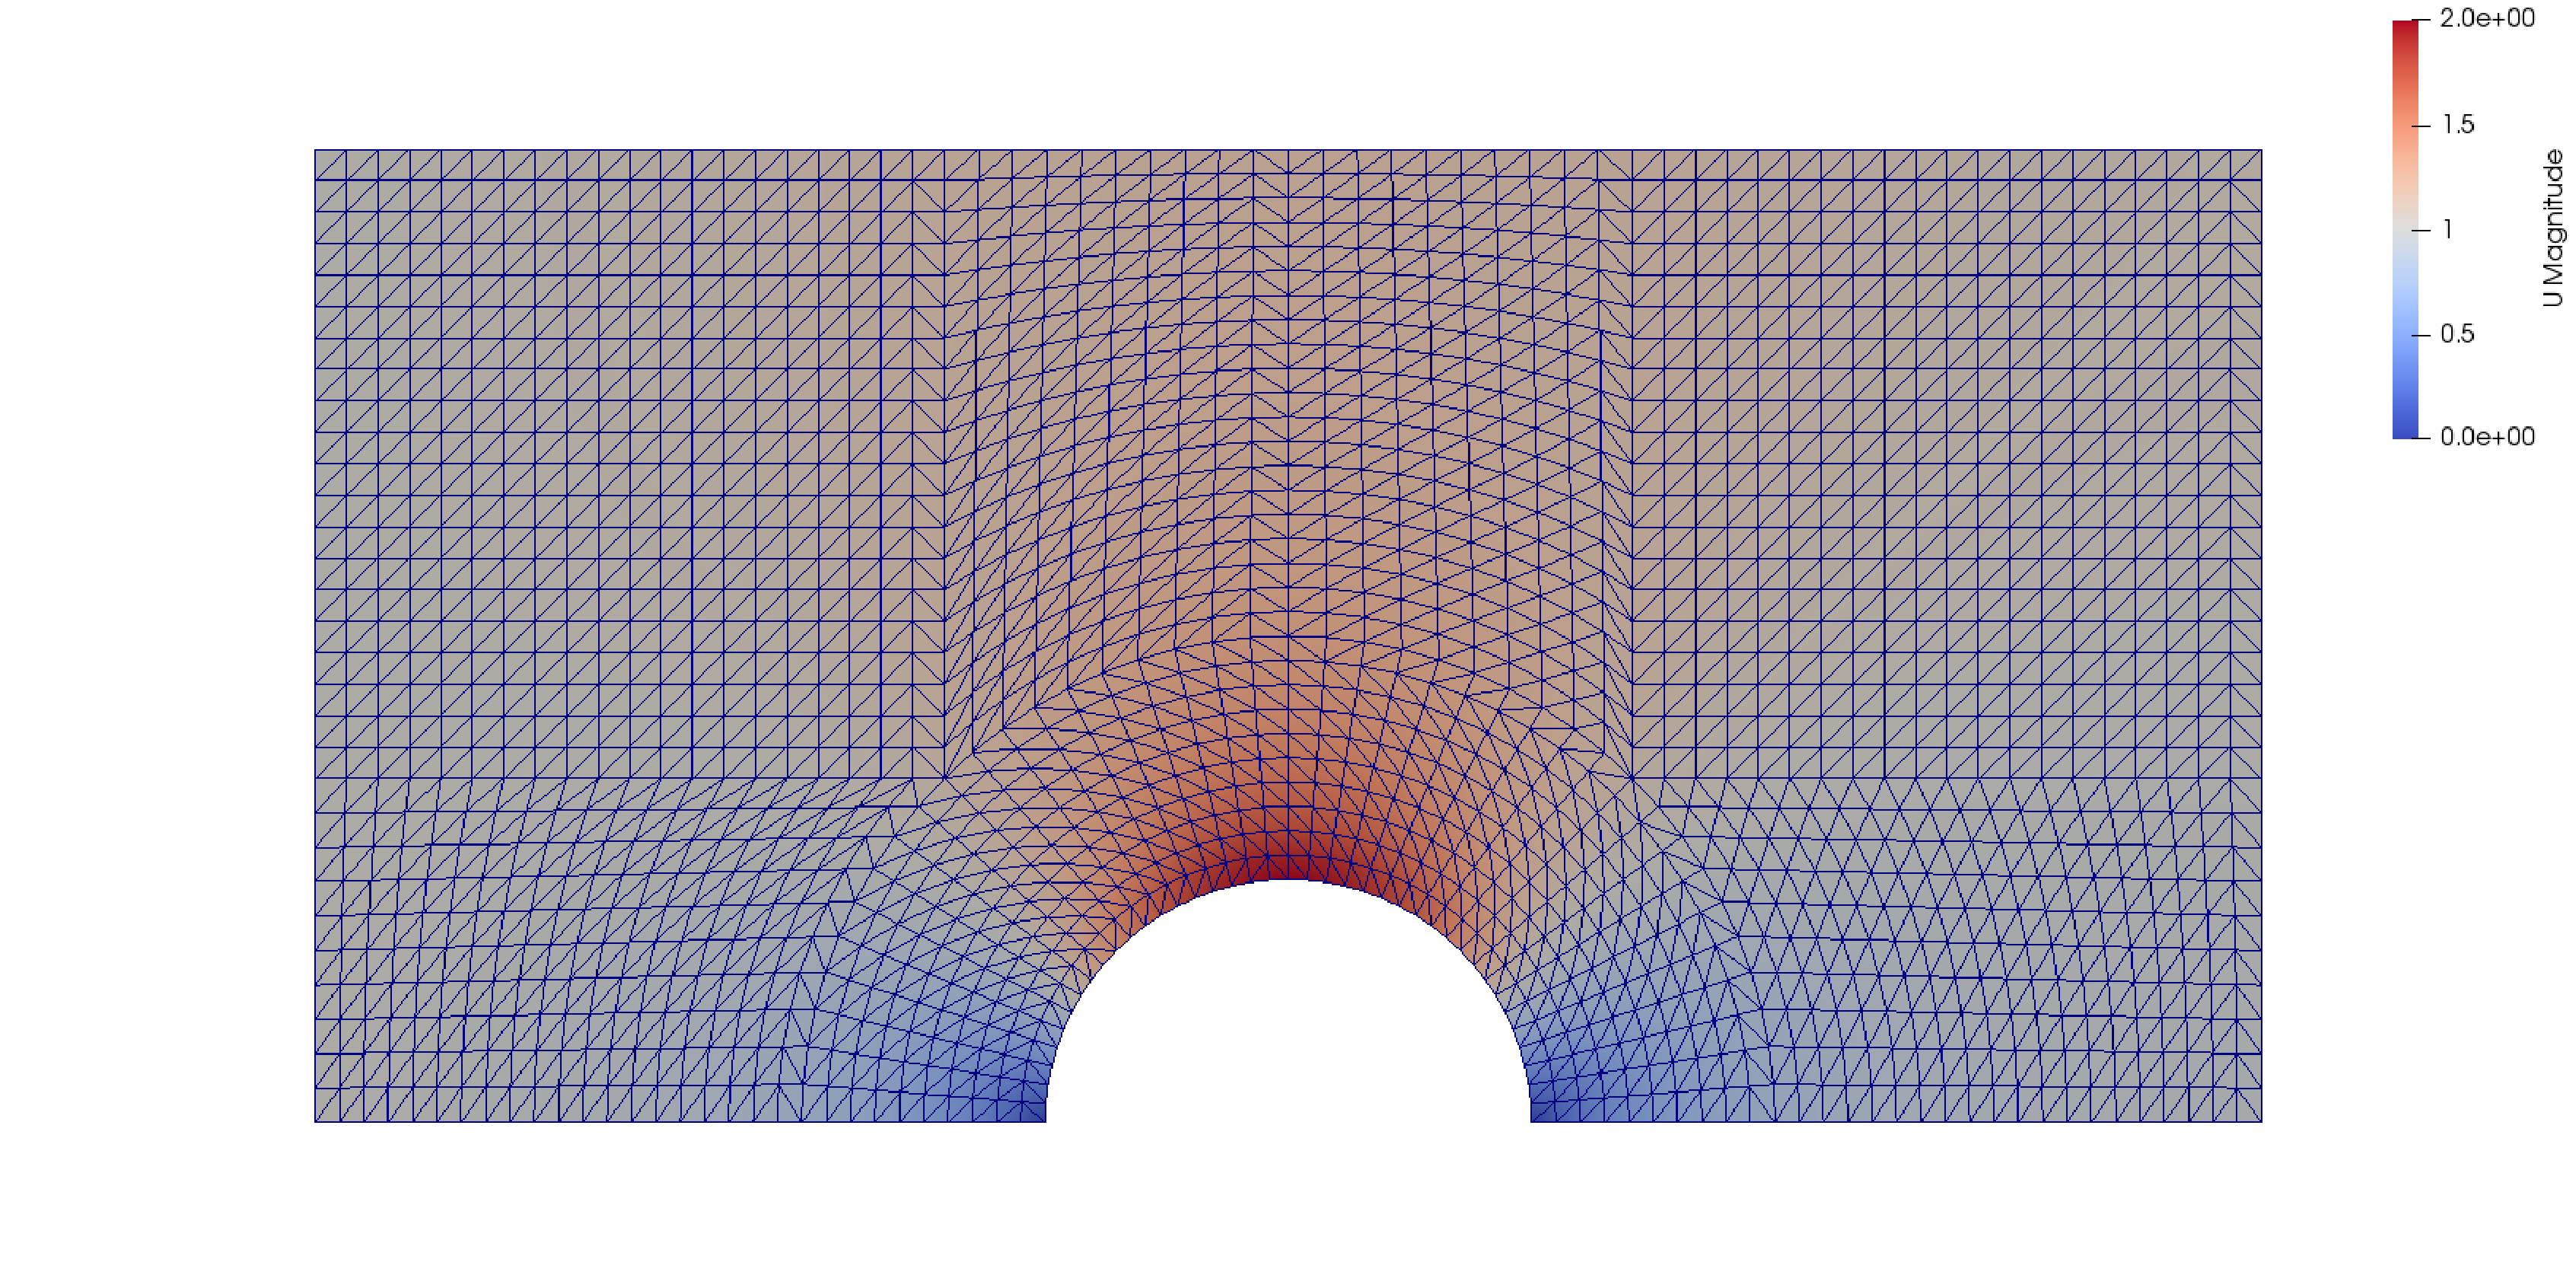
\includegraphics[trim={250 100 250 100},clip, width=\textwidth]{images/Velocity_mesh.pdf}
    \tiny{Velocity and computational grid}
    \caption{\footnotesize Cylinder potential flow}
    \label{fig:OpenFoam}
    \end{figure}
    
    
    \end{column}
    \end{columns}

\end{frame}{}

\begin{frame}{Medical data: Head scan}
    
    \begin{columns}[t]
    \begin{column}{0.5\linewidth}
    3D image file. Download \href{https://github.com/MrGeislinger/leapmotion-paraview/blob/master/Examples/ParaViewTutorialData/headsq.vti}{\bf\underline{headsq.vti}}
    \begin{itemize}
        \item VTKFile with XML formats
        \item Binary image data
    \end{itemize}{}
    
    \end{column}
    
    \begin{column}{0.5\linewidth}
    
    \begin{figure}
    \centering
    \captionsetup{labelformat=empty}
    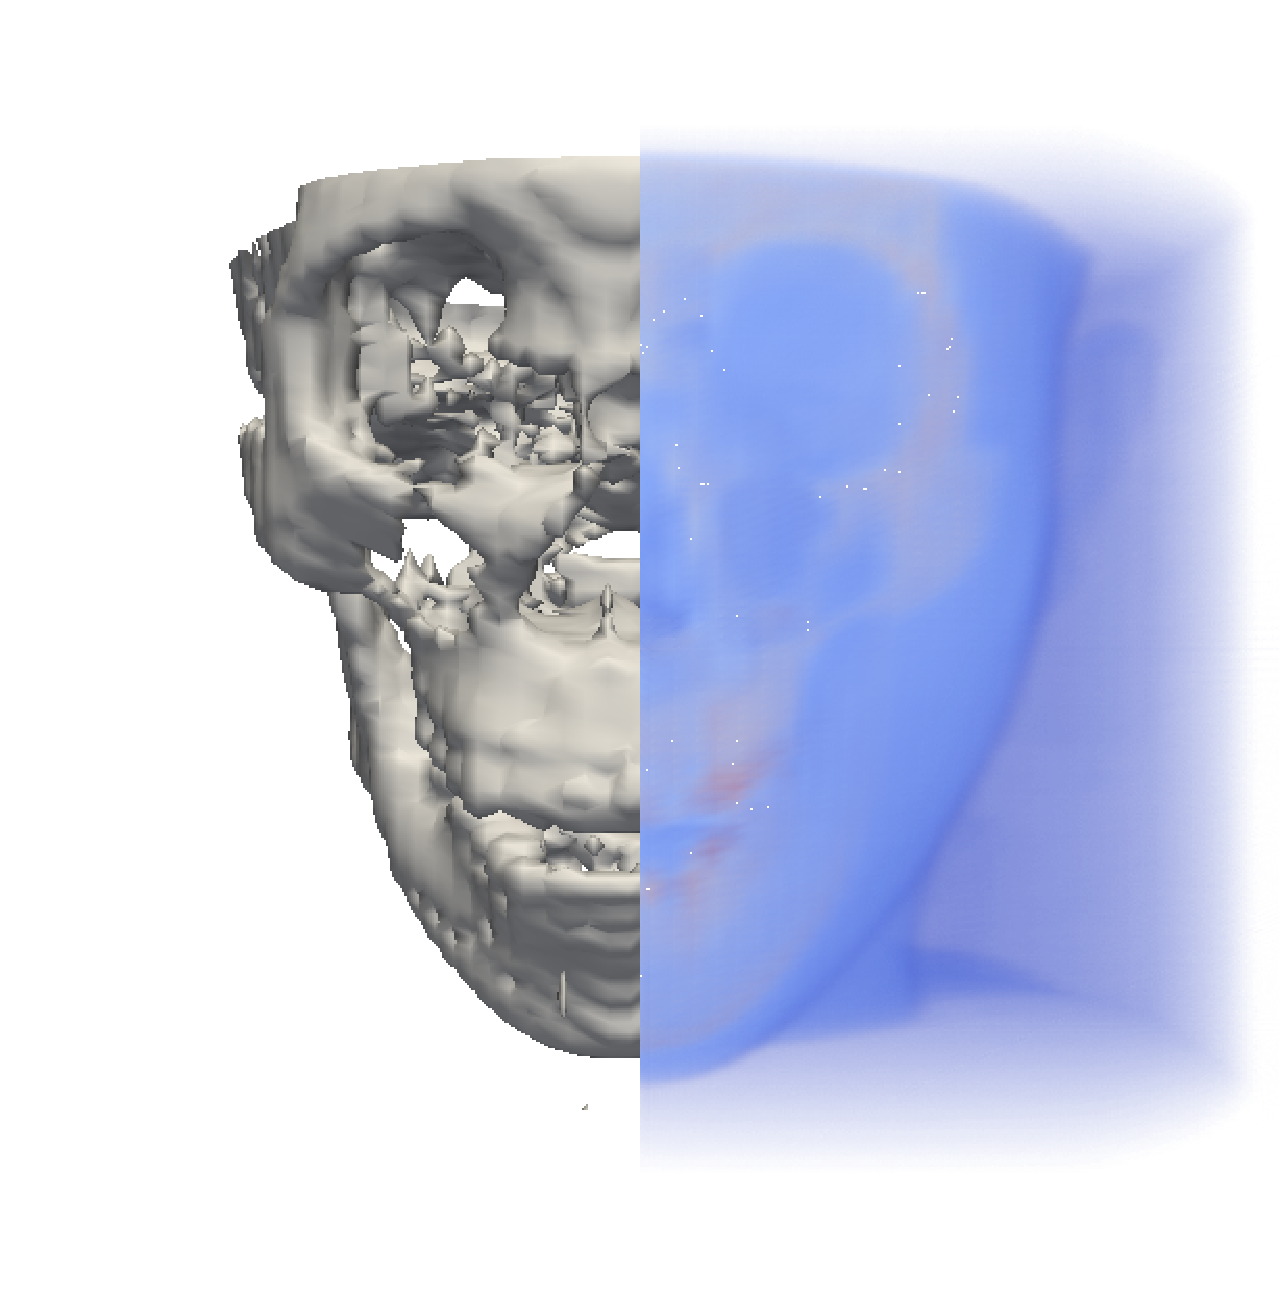
\includegraphics[width=\textwidth]{images/headsq.pdf}
    \caption{\footnotesize Data from head scan}
    \label{fig:headsq}
    \end{figure}
    
    \end{column}
    
    \end{columns}
    
\end{frame}{}

\begin{frame}{Exercises: Day 2}
    For Exercise 2.19, load \texttt{can.ex2} from \texttt{ParaView-v5.8.0-RC1/Testing/Data/}
    \begin{itemize}
        \item Explore all the different options as you go along
        \item If you finish, create document with image output
    \end{itemize}


\end{frame}{}

\section{Exercises; ParaView database and OpenFOAM}

\begin{frame}{Exercises: Day 3}

\small

To prepare for the evaluation exercise:
\begin{itemize}
    \item Use data (ParaView examples, internet, simulation software, e.g. OpenFOAM tutorials,...)
    \item Create images, videos, etc then put in document (good formatting, e.g. correct font sizes, etc)
    \item Create plots / analysis to show interesting behaviour or phenomena
\end{itemize}{}

Work on several data-sets throughout the day. Discuss the results in groups and show me what you have found. Ideas for data sources:
\begin{itemize}
    \item (morning) ParaView example data
    \begin{itemize}
        \item AMR {\tiny\texttt{amr/spcth.0}, tutoral \href{https://docs.paraview.org/en/latest/Tutorials/ClassroomTutorials/targetedParaViewAndCTH.html#targeted-paraview-cth}{\underline{here}}}
        \item Aerofoil {\tiny\texttt{EnSight/naca.bin.case}}
        \item Iron protein(?) {\tiny\texttt{Iron\_Xdmf/Iron\_Protein.ImageData.Collection.xmf}}
        \item \href{https://www.rcsb.org/structure/3GQP}{\bf\underline{3GQP}} protein {\tiny\texttt{/3GQP.pdb}}
    \end{itemize}{}
    \item (afternoon) OpenFoam tutorials \href{https://www.openfoam.com/documentation/tutorial-guide/}{\bf\underline{here}}, other 3D simulation software
    \item Other possibilities; create sources to demonstrate animations, mathematical geometric data, ...
\end{itemize}{}

\end{frame}{}

\begin{frame}{OpenFOAM data}
    
    \begin{enumerate}
        \item {\bf Cavity flow tutorial;} obtain \texttt{cavity.zip} (with documentation \href{https://www.openfoam.com/documentation/tutorial-guide/}{\bf\underline{here}}) and open in ParaView, then apply filters (glyph, streamline, plot velocity profile along centre line). After output images and use in a document to make descriptions of the flow
        \item {\bf Dam break tutorial;} obtain \texttt{damBreak.zip} and open in paraView. Then create an animation and use to describe what is happening in the simulation, then find the maximum pressure on the right hand wall : \href{https://www.openfoam.com/documentation/tutorial-guide/tutorialse8.php#x14-680004.1}{\bf\underline{damBreak}}
    \end{enumerate}{}
    
\end{frame}{}

\begin{frame}{Batch scripting: Day 4}
    
    Python scripting can be leveraged in two ways within ParaView:
    \begin{enumerate}
        \item Automate the setup and execution of visualisations by performing the same actions as a user at the GUI
        \item Run inside pipeline objects, thereby performing parallel visualisation algorithms
    \end{enumerate}
    
    \vskip 6 pt
    
    Good way to automate mundane and repetitive tasks
    
    \vskip 6pt
    
    Critical component when using ParaView in situations where the GUI is undesired or unavailable
    
    \vskip 6pt
    
    Python scripting to establish \emph{in situ} computation within simulation code, i.e. script included in simulation code
    
    \vskip 6pt
    
    Scripting allows access to much wider range of capabilities

\end{frame}{}

\begin{frame}{Python}

From \href{https://www.python.org/}{\bf\underline{Python.org}}: \quad\emph{``Python is a programming language that lets you work quickly and integrate systems more effectively''}

\vskip 6pt

Open-source and freely available

\vskip 6pt

Good for beginners and those experienced with other languages

\vskip 6pt

Both Python's standard library and the community-contributed modules allow for endless possibilities. Libraries include:
\begin{itemize}
    \item \href{https://numpy.org/}{\bf\underline{NumPy}}  is the fundamental package for scientific computing
    \item \href{https://matplotlib.org/}{\bf\underline{matplotlib}} is a comprehensive library for creating static, animated, and interactive visualisations
\end{itemize}{}

\vskip 6pt

Runs from command line and can be scripted
\begin{itemize}
    \item Basic demonstration
\end{itemize}

\end{frame}{}


\begin{frame}{Scripting approaches}
    
    \begin{description}
        \item[Python Shell] Find in \texttt{View} $\rightarrow$ \texttt{Python Shell}
        \item[pvpython] Runs on command line for interactive scripts
        \item[pvbatch] Runs on the command line for batch processing. Can be run in parallel
        \item[pvserver] For remote visualization, useful on HPC resources
    \end{description}{}
    
    \vskip 6pt
    
    There are also programmable sources and filters...
    

\end{frame}{}

\begin{frame}{Programmable filter example}

    \begin{itemize}
        \item Apply a programmable filter to file1.vtk (day 2)
    \end{itemize}

    {
    \small
    \lstinputlisting[language=Python]{code/programmable_filter.py}
    }

    \begin{figure}
    \centering
    \captionsetup{labelformat=empty}
    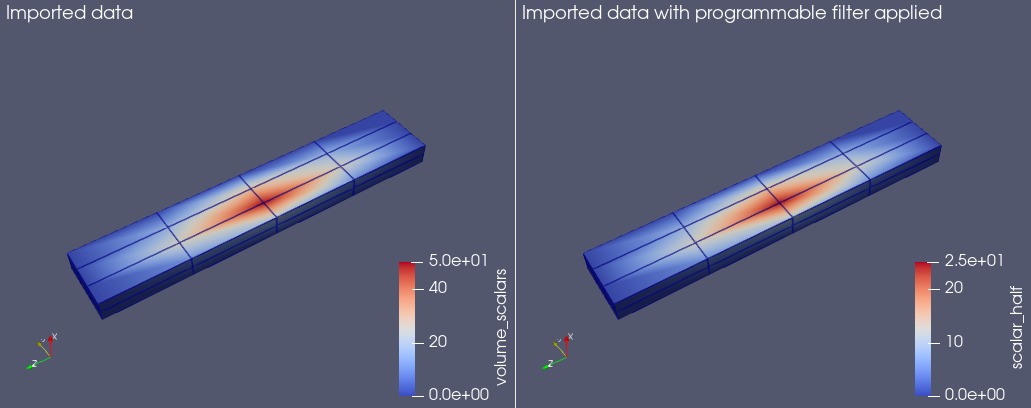
\includegraphics[trim={0 0 0 0},clip, width=\textwidth]{images/programmable_filter.png}
    \caption{\footnotesize Programmable filter applied to structured vtk file}
    \label{fig:programmable_filter}
    \end{figure}

\end{frame}{}

\begin{frame}{Programmable source example}

    \begin{itemize}
        \item Use data.csv to create a programmable source (day 1)
    \end{itemize}

    {
    \tiny
    \lstinputlisting[language=Python]{code/programmable_source.py}
    }

    \begin{figure}
    \centering
    \captionsetup{labelformat=empty}
    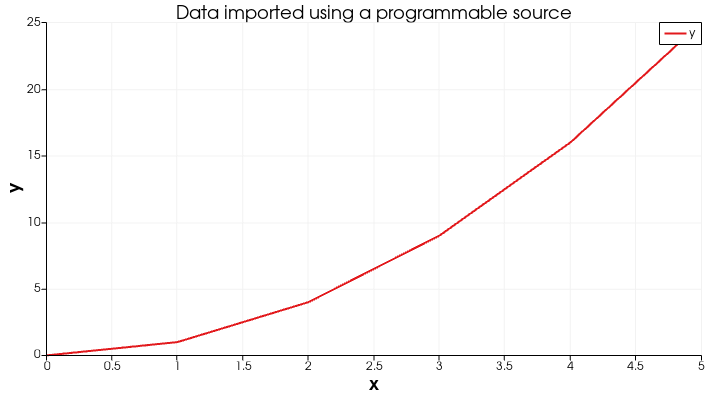
\includegraphics[trim={0 0 0 0},clip, width=0.6\textwidth]{images/programmable_source.png}
    \caption{\footnotesize Programmable source applied to csv data file}
    \label{fig:programmable_source}
    \end{figure}

    
\end{frame}{}


\begin{frame}{Programmable sources and filters}


    \begin{itemize}
        \item Try the other examples given here \href{https://docs.paraview.org/en/latest/ReferenceManual/pythonProgrammableFilter.html}{\bf\underline{here}}, adjust the code to see what changes
    \end{itemize}{}
    \begin{figure}
    \centering
    \captionsetup{labelformat=empty}
    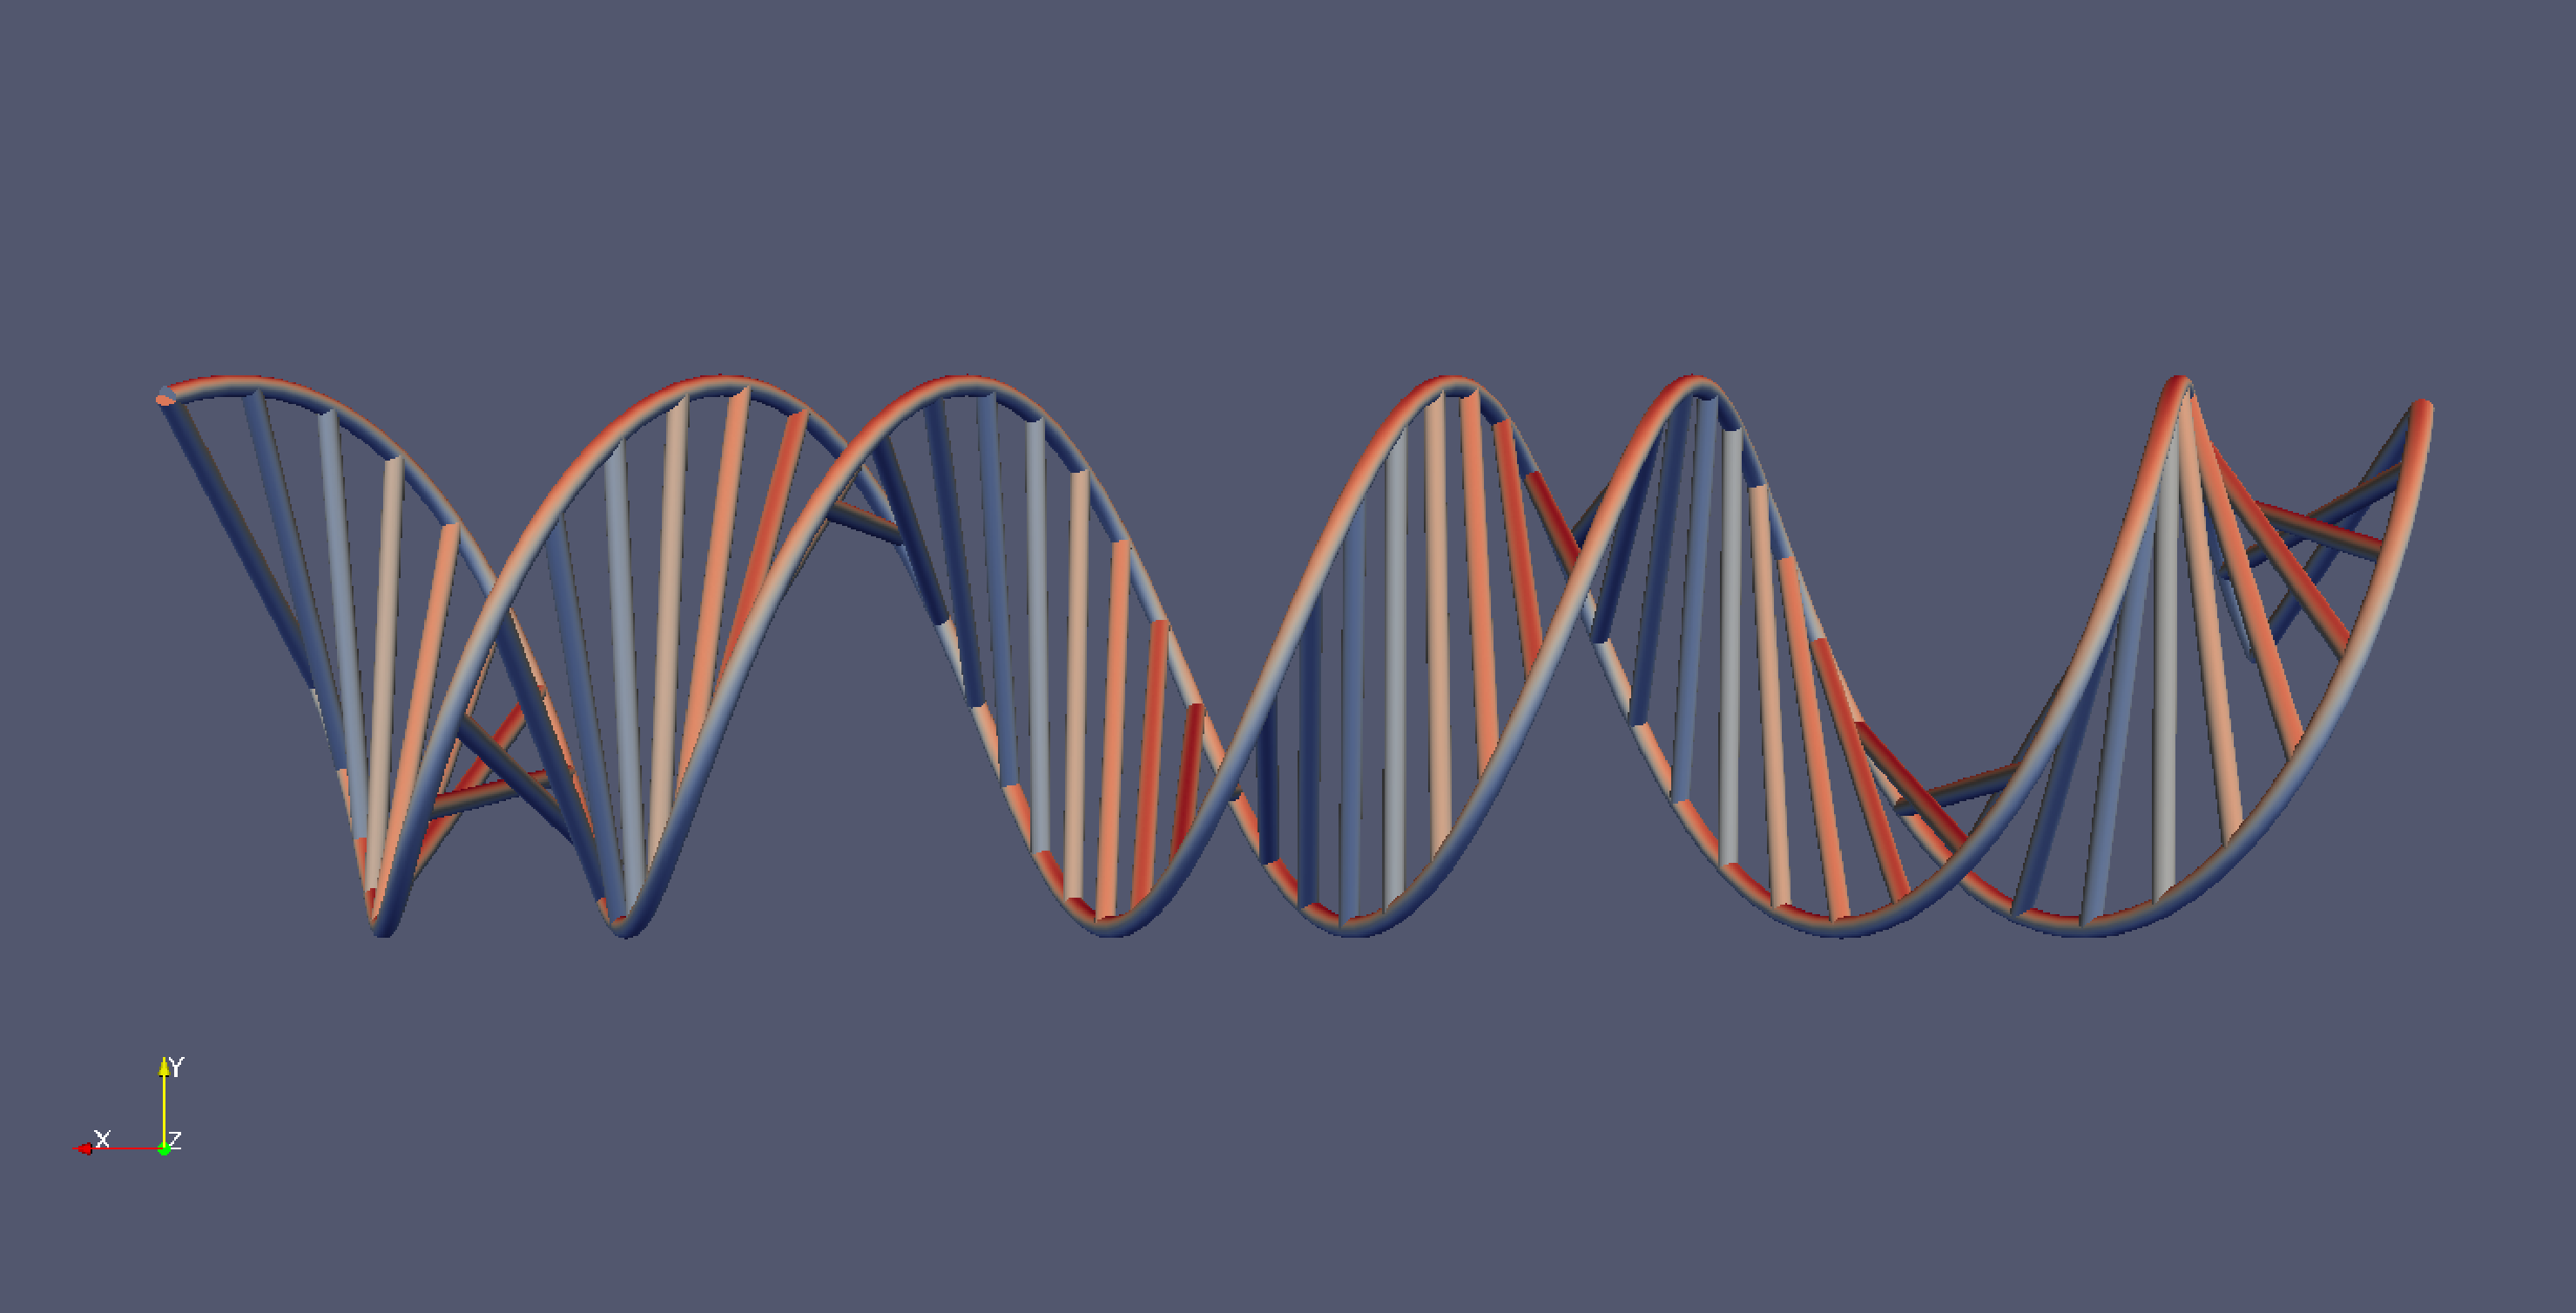
\includegraphics[trim={0 150 0 150},clip, width=0.7\textwidth]{images/DoubleHelix.pdf}
    \caption{\footnotesize Double helix created with programmable source}
    \label{fig:DoubleHelix}
    \end{figure}


\end{frame}{}


\begin{frame}{Tracing actions for scripting}
    
    For tracing actions in the UI as a Python script
    \begin{itemize}
        \item \texttt{Tools} $\rightarrow$ \texttt{Start Trace}
        \item Execute a series of actions in the UI
        \item \texttt{Tools} $\rightarrow$ \texttt{Stop Trace}
    \end{itemize}{}
    Produces a python script that corresponds to performed actions
    
    \vskip 6pt
    
    Save script and use for batch processing
    
    \vskip 6pt
    
    Good way to discover ParaView python commands and syntax
    
\end{frame}{}

\section{Python scripting}

\begin{frame}{Exercises: Day 4}
    Exercises in chapter 3 of the ParaView tutorial on scripting  
    
    \vskip 24pt
    
    Create a script that outputs an annotated visualisation including filters, and a plot over line, from day 3 OpenFoam excercises, e.g. cavity flow tutorial. After, run this in a terminal using \$ pvpthon script.py (note, may be necessary to put Interact() at the end of the script)
\end{frame}{}

\begin{frame}{Other scripting possibilities}
    \begin{itemize}
        \item \href{https://docs.pyvista.org/}{\underline{PyVista}} 3D plotting and mesh analysis through a streamlined interface for the Visualization Toolkit (VTK)
        \begin{itemize}
            \item No GUI
            \item Lighter than ParaView
            \item Some filters that are not included in ParaView, e.g. \href{https://docs.pyvista.org/api/core/_autosummary/pyvista.UnstructuredGridFilters.delaunay_2d.html}{delaunay_2d} to construct mesh from data points
        \end{itemize}
        \item VTK in \href{https://kitware.github.io/vtk-examples/site/Python/GeometricObjects/Cylinder/}{\underline{python}}
        \begin{itemize}
            \item No GUI, hence necessary to develop script from online examples and python commands
        \end{itemize}
        \item VTK in \href{https://kitware.github.io/vtk-examples/site/Cxx/GeometricObjects/Cylinder/}{\underline{c++}}
        \begin{itemize}
            \item No GUI, need for make/cmake files
            \item Allows access to whole VTK library
            \item Useful for full integration into simulation code, e.g. \href{https://www.cfdem.com/liggghts-open-source-discrete-element-method-particle-simulation-code}{\underline{Liggghts}}
        \end{itemize}
    \end{itemize}
\end{frame}{}

\begin{frame}{Creating dashboards}

A useful way to allow non-expert users to manipulate a visualisation

\begin{center}
    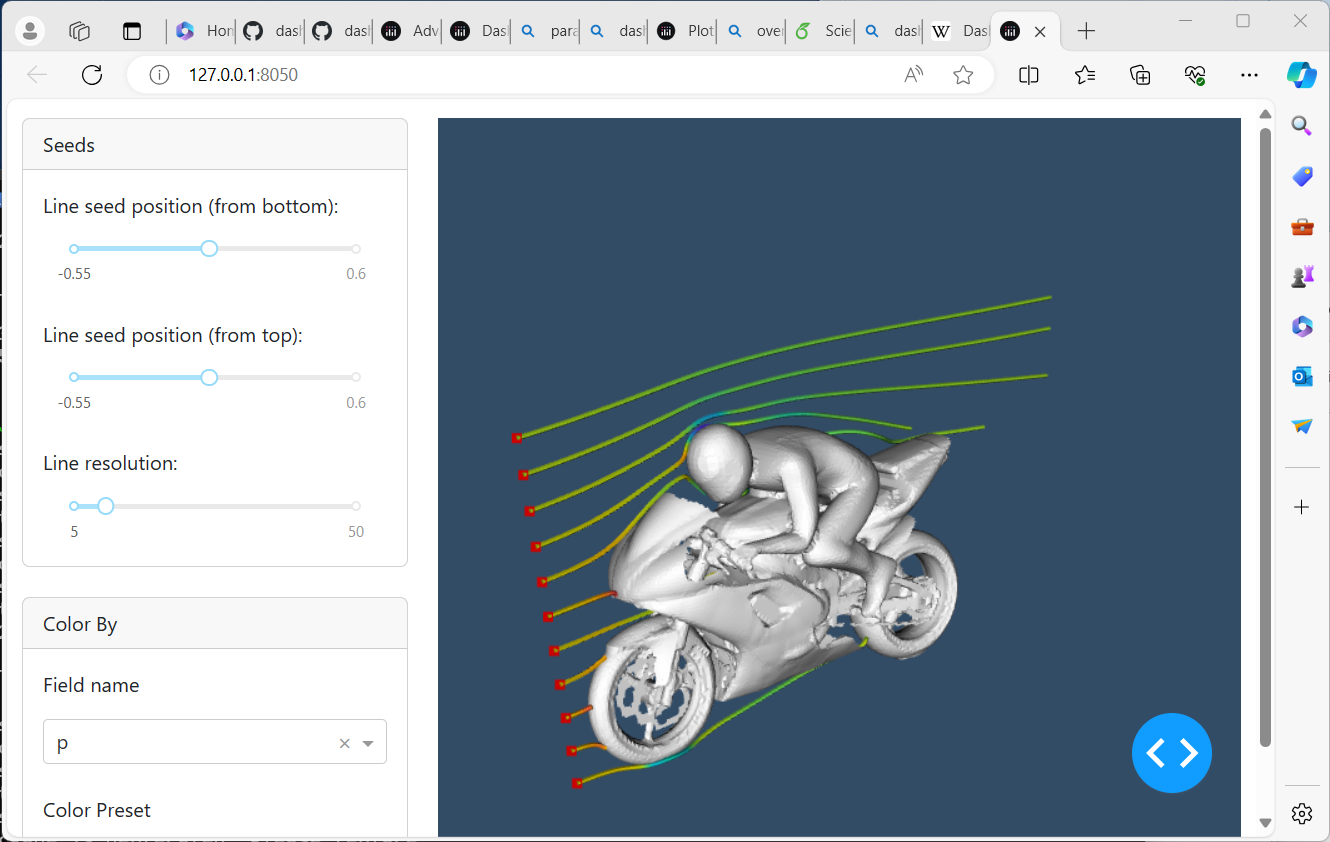
\includegraphics[width=0.7\linewidth]{images/motorbikeDashboard.png}
\end{center}

Try to install and run this \href{https://github.com/johnsgit9/dashvis.git}{\underline{small example}}.

\vskip 6pt

For some advanced, but illustrative, plotly examples, see \href{https://dash.plotly.com/vtk/advanced}{\underline{here}}.

\end{frame}

\section{Visualising large models}

\begin{frame}{Visualising large models}
    
    ParaView used at institutions around the world to visualise data from large-scale simulations run on the world's largest supercomputers
    
    \vskip 12pt
    
    \begin{inlinefig}
    \begin{tabular}{cc}
    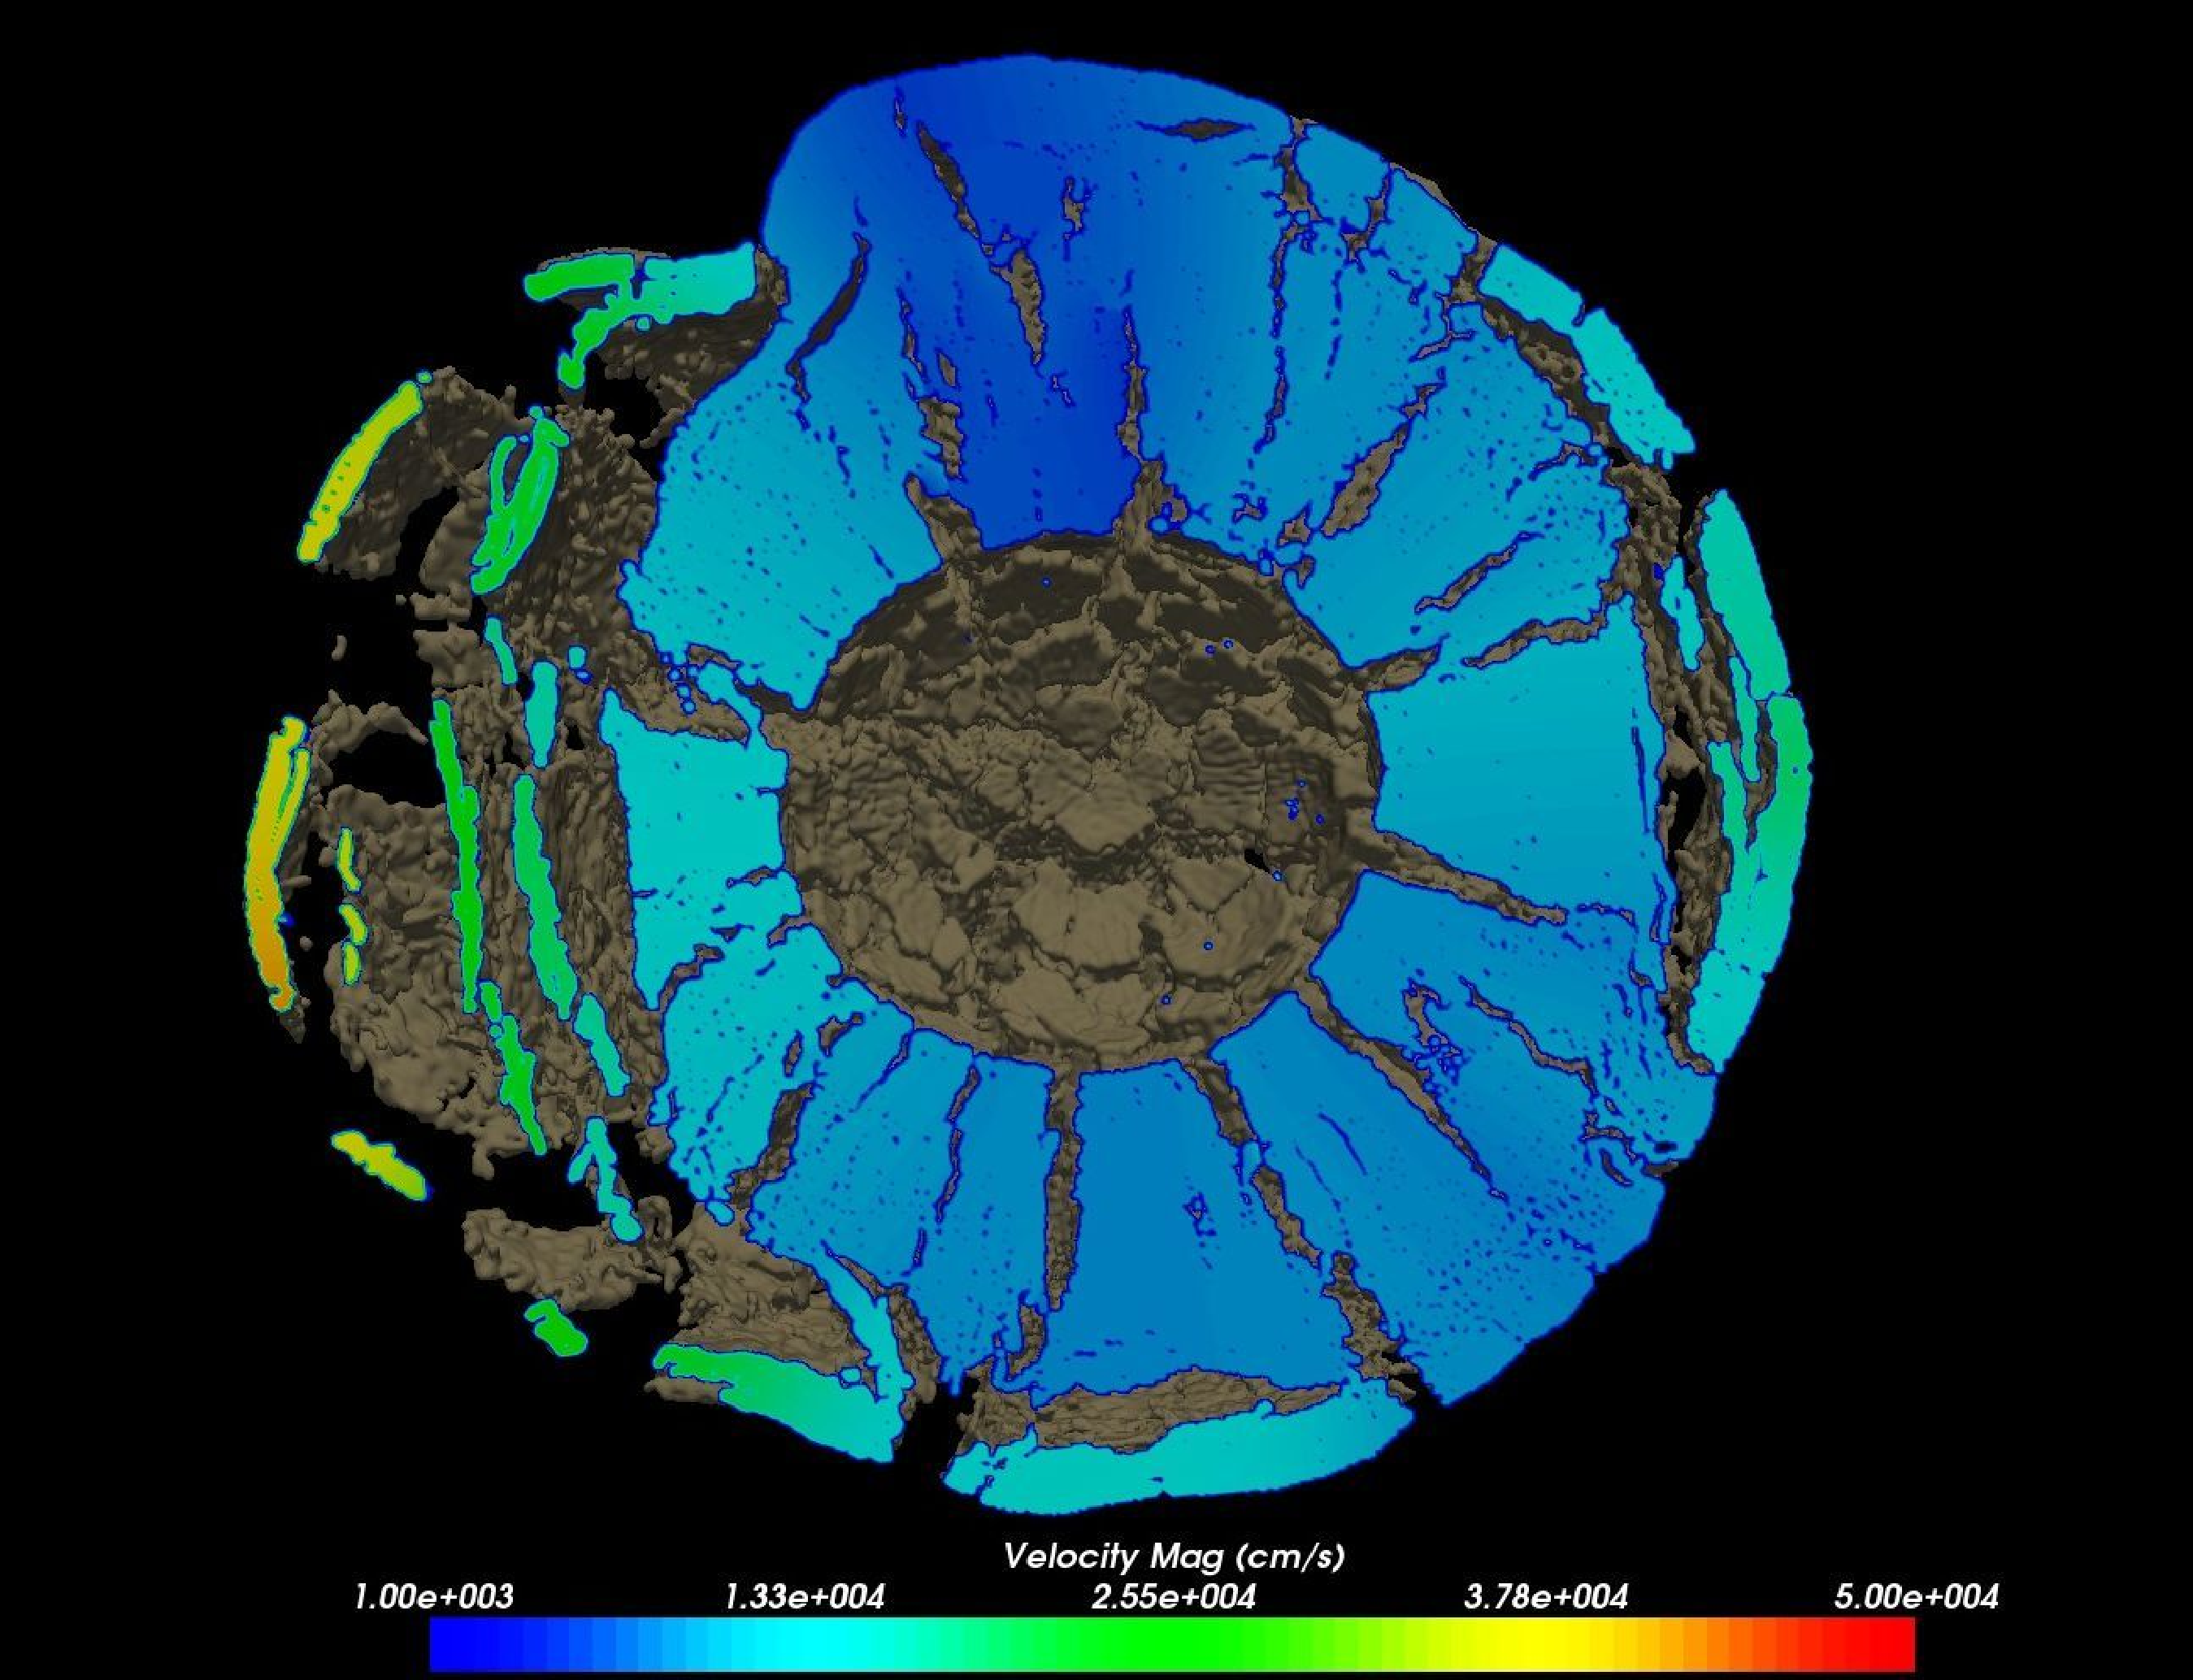
\includegraphics[width=0.431\linewidth]{images/Asteroid} &
    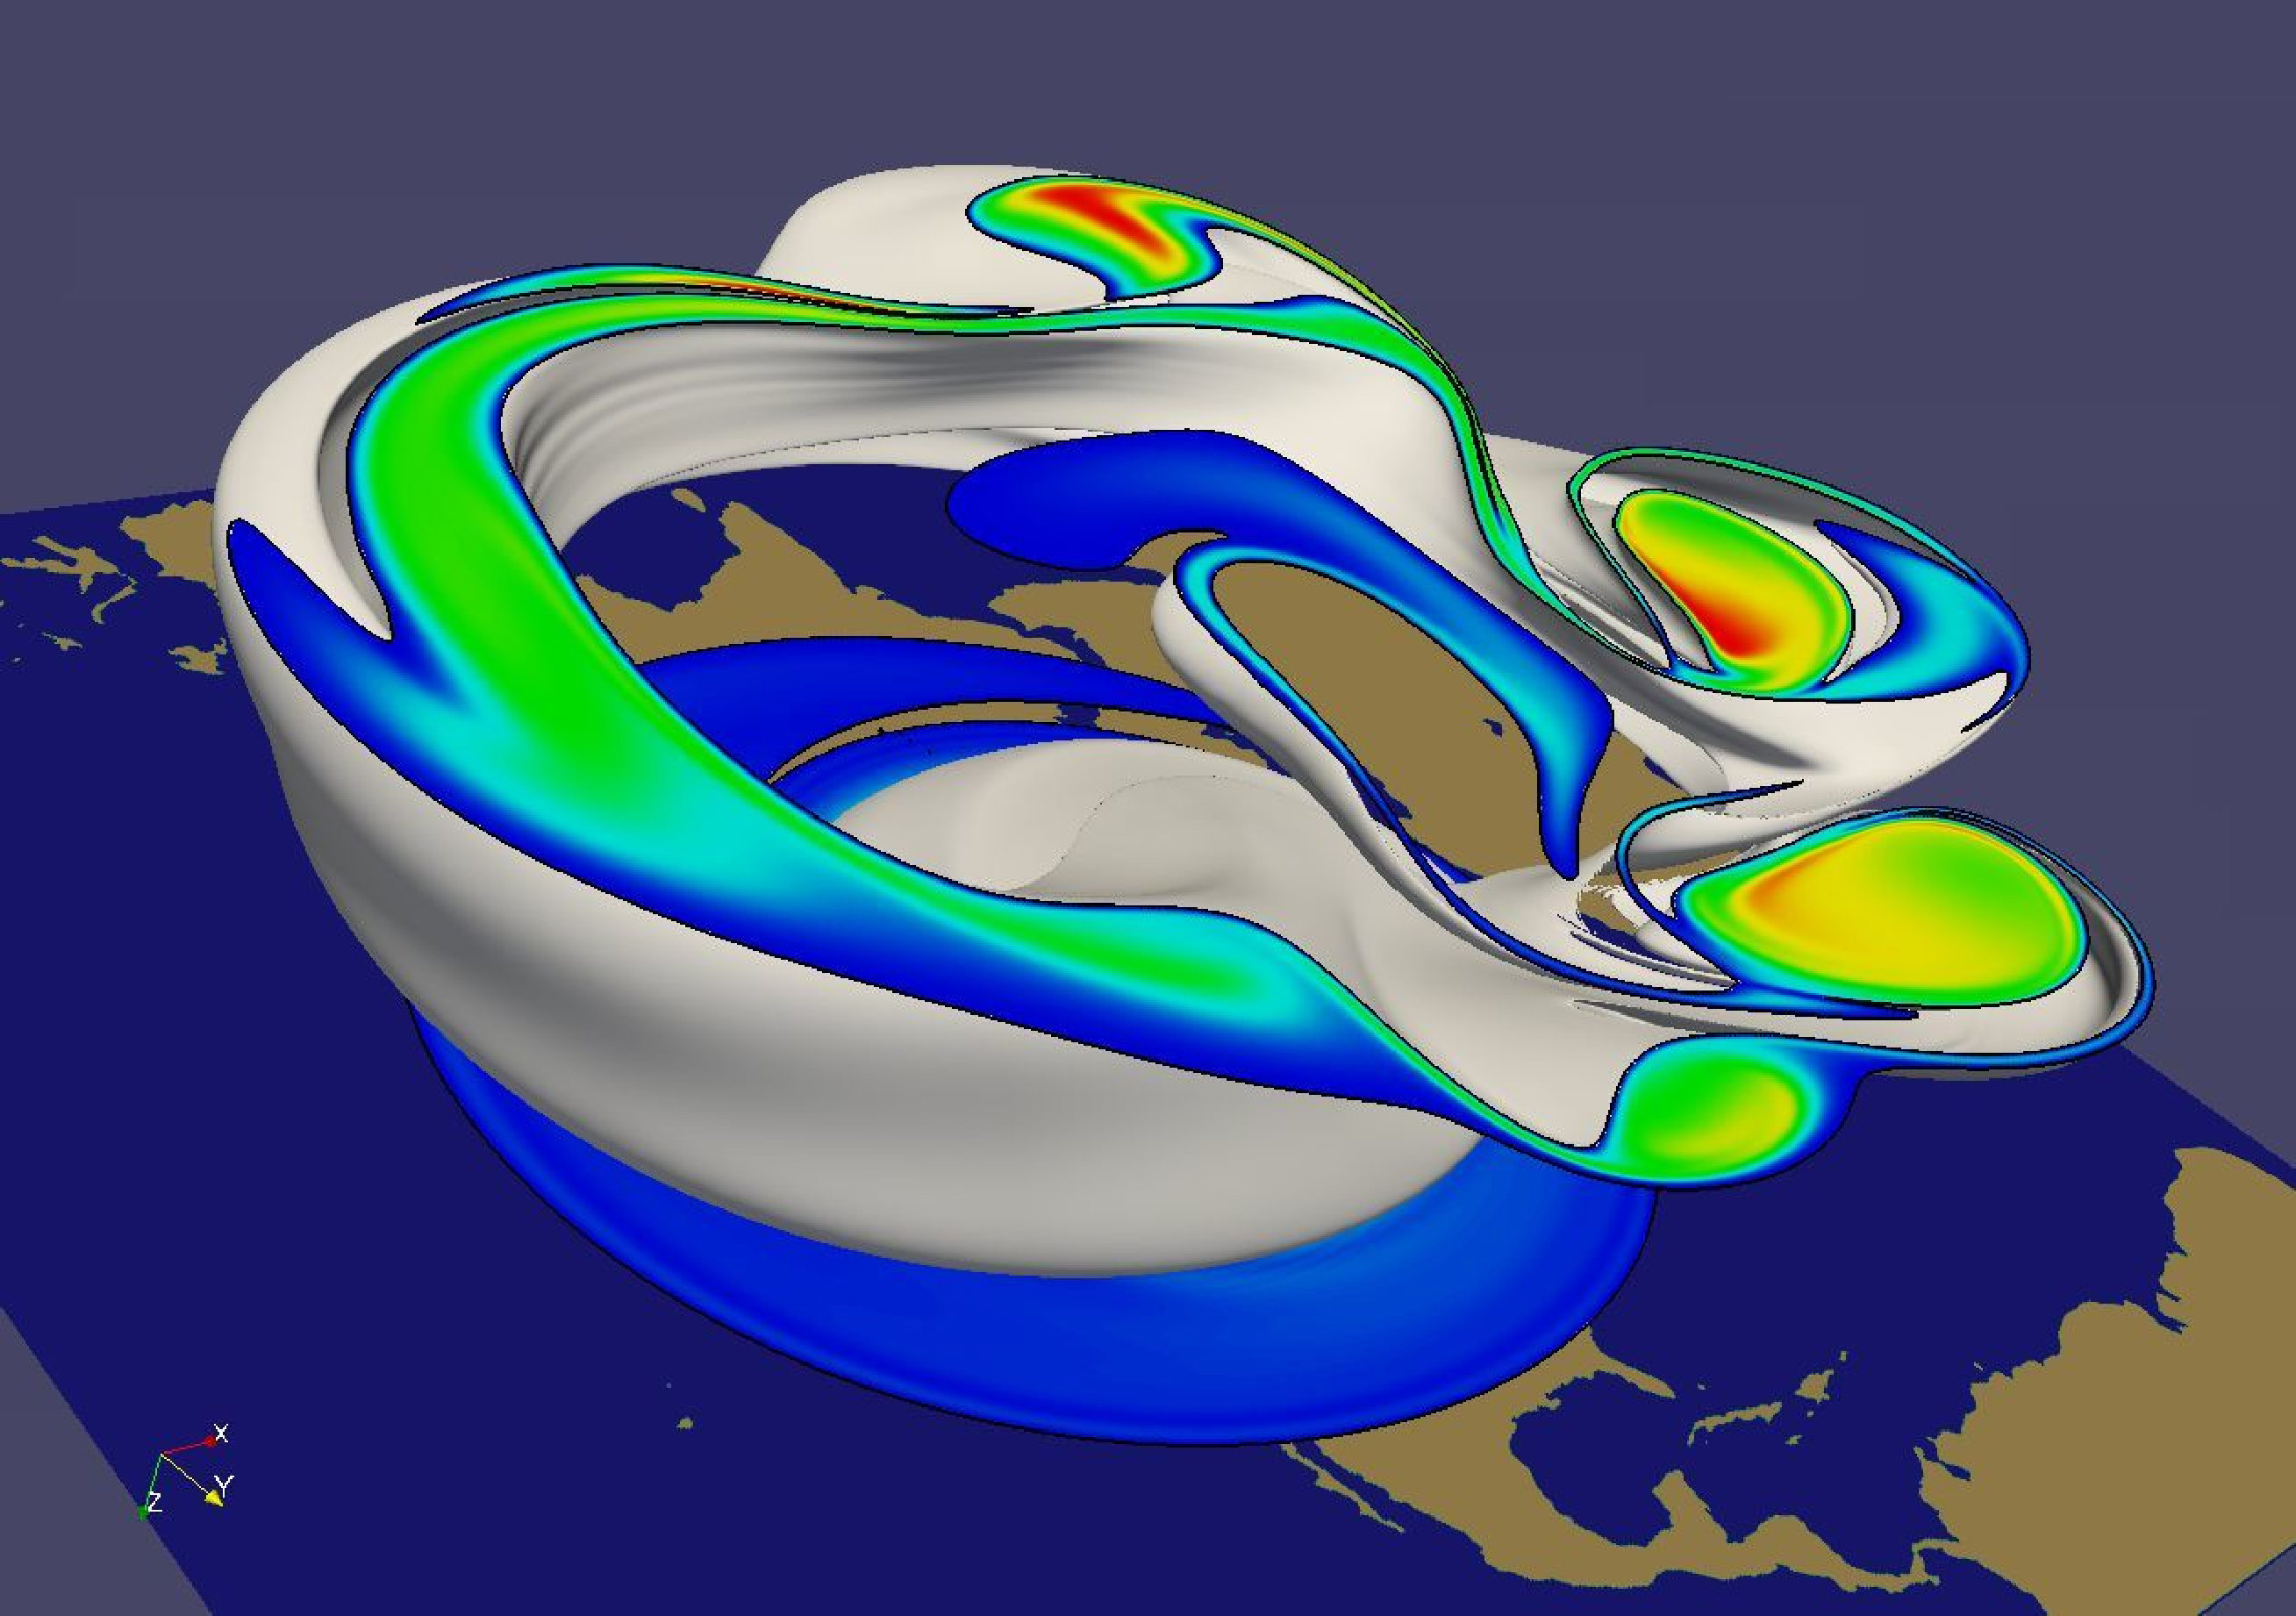
\includegraphics[width=0.469\linewidth]{images/PolarVortex} \\
    \parbox[t]{0.431\linewidth}{\footnotesize CTH shock physics simulation
      with over 1 billion cells of a 10 megaton explosion detonated at the centre of the Golevka asteroid} &
    \parbox[t]{0.469\linewidth}{\footnotesize SEAM Climate Modeling simulation with 1 billion cells modeling the breakdown of the polar vortex, a circumpolar jet that traps polar air at high latitudes}
    
  \end{tabular}
\end{inlinefig}
\end{frame}    
    \begin{frame}{Visualising large models}
    
    \begin{inlinefig}
    \begin{tabular}{cc}
    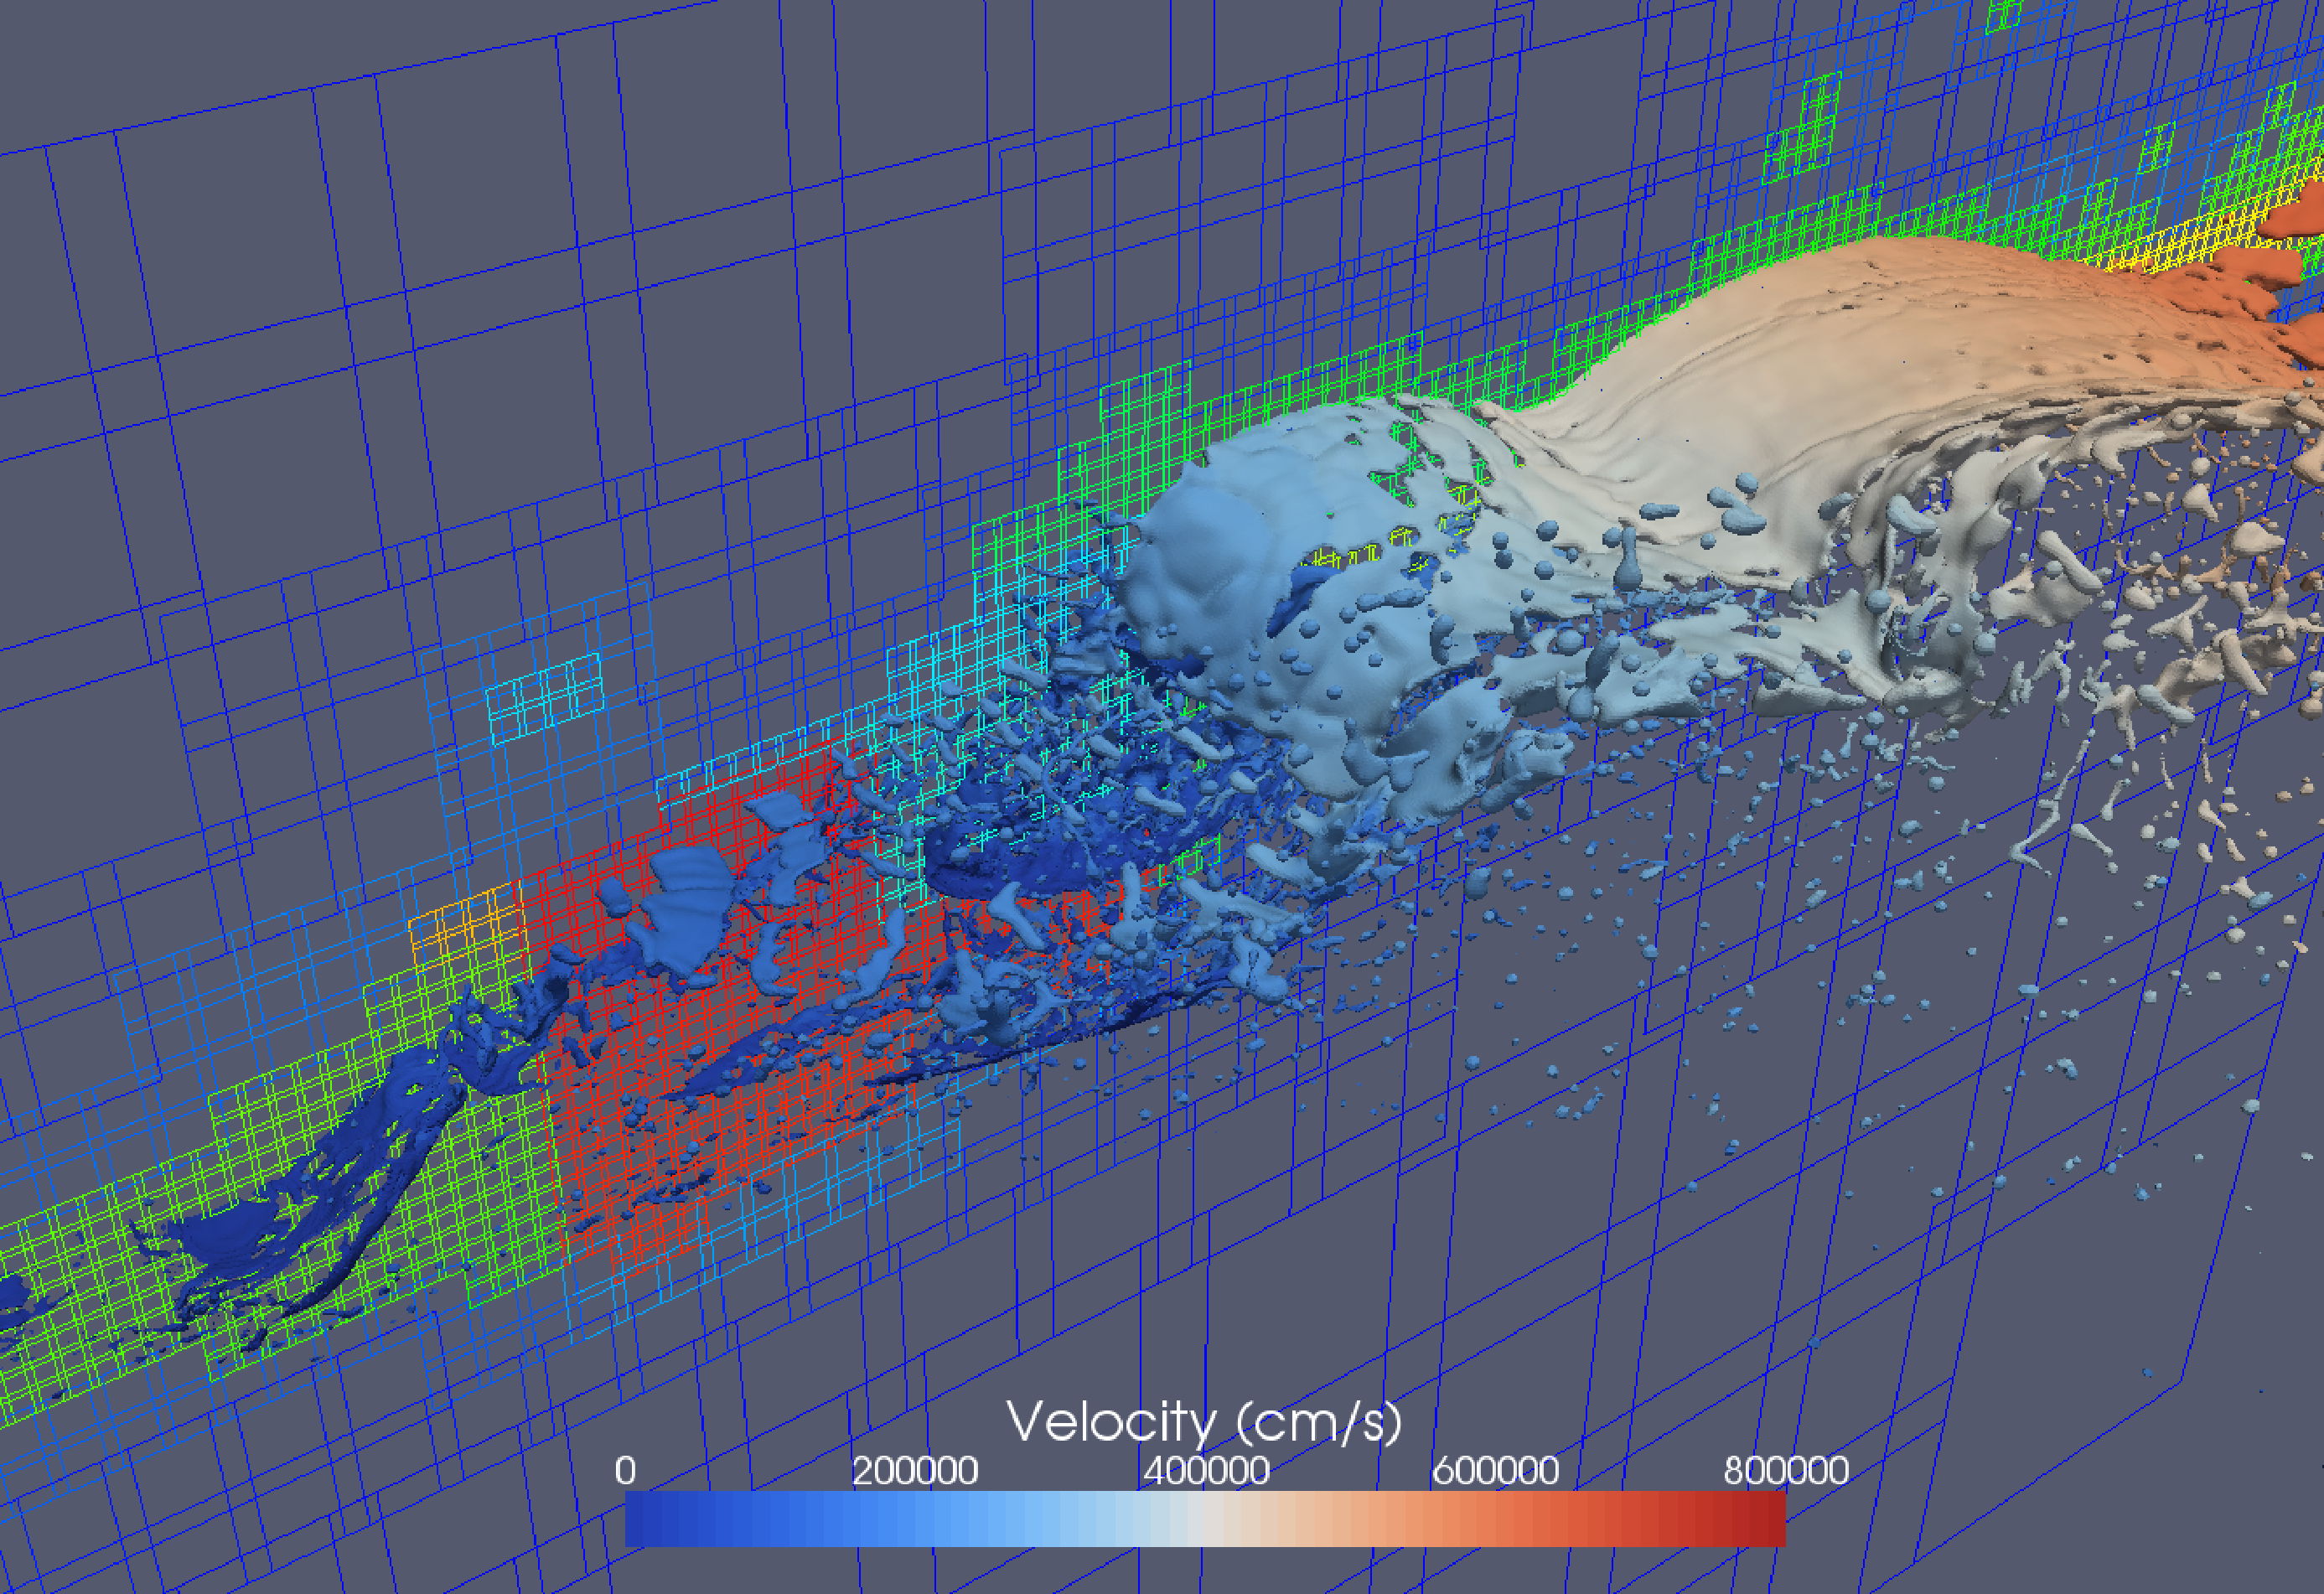
\includegraphics[width=0.474\linewidth]{images/LargeAMR} &
    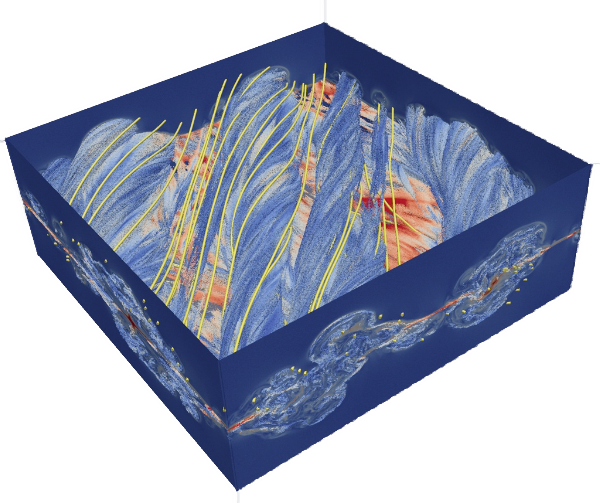
\includegraphics[width=0.426\linewidth]{images/vpic} \\
    \parbox[t]{0.474\linewidth}{\footnotesize A CTH simulation that generates AMR data. ParaView has been used to visualize CTH simulation AMR data comprising billions of cells, 100's of thousands of blocks, and eleven levels of hierarchy (not shown)} &
    \parbox[t]{0.426\linewidth}{\footnotesize A VPIC simulation of magnetic reconnection with 3.3 billion structured cells}
  \end{tabular}
\end{inlinefig}
\end{frame}

\begin{frame}{Visualising large models}
    
\begin{inlinefig}

  \begin{tabular}{cc}
    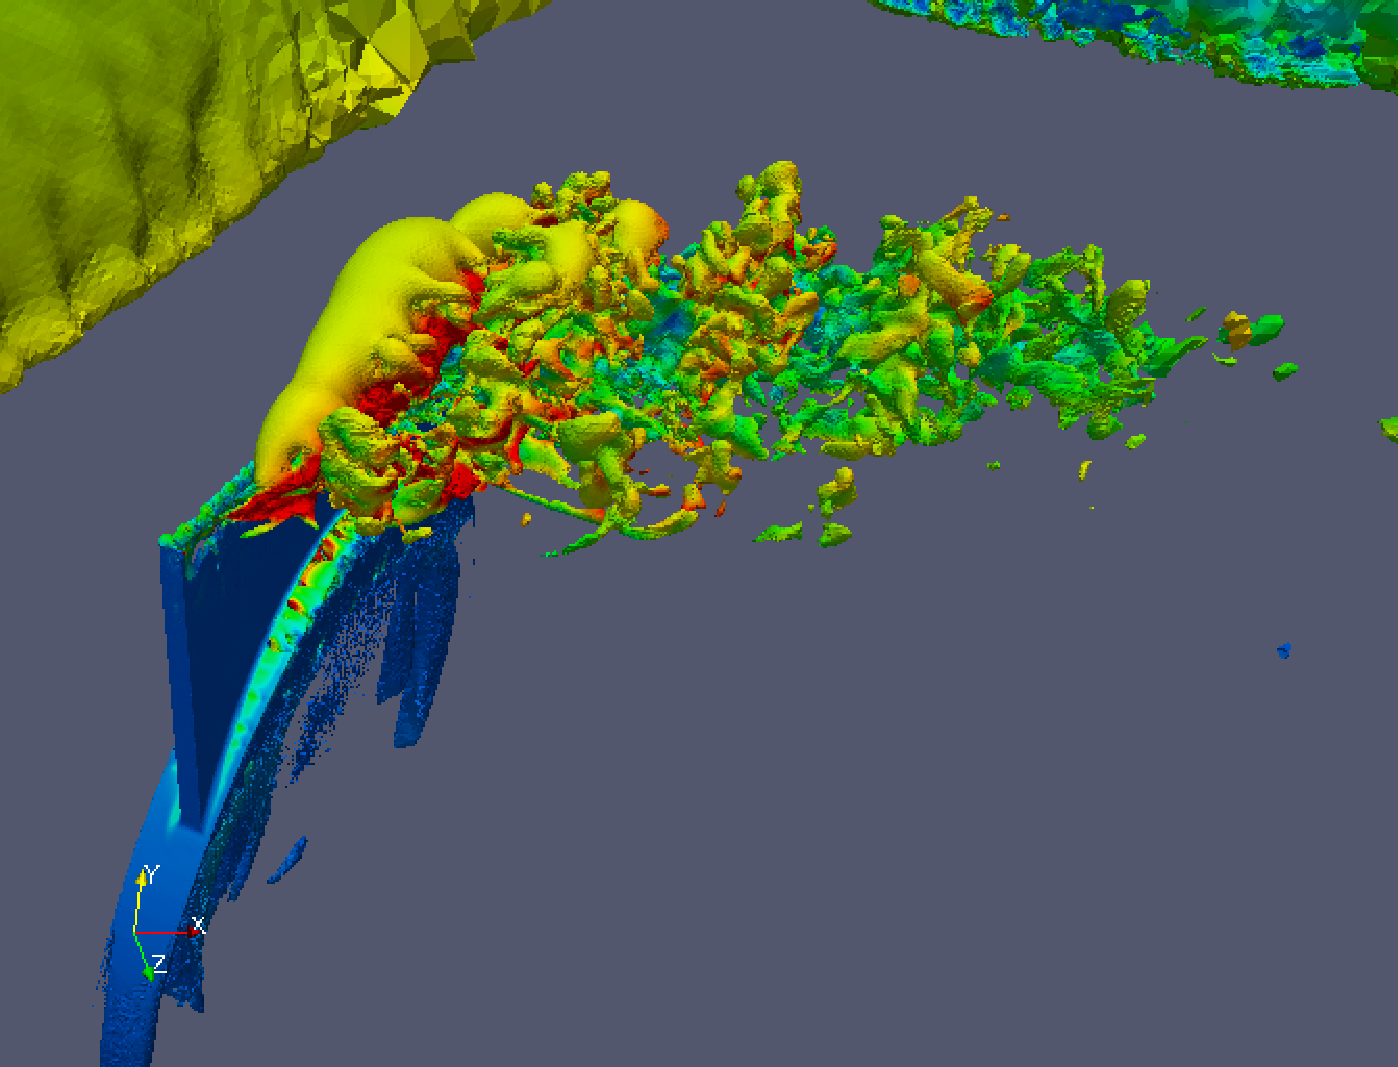
\includegraphics[width=0.383\linewidth]{images/Crossflow} &
    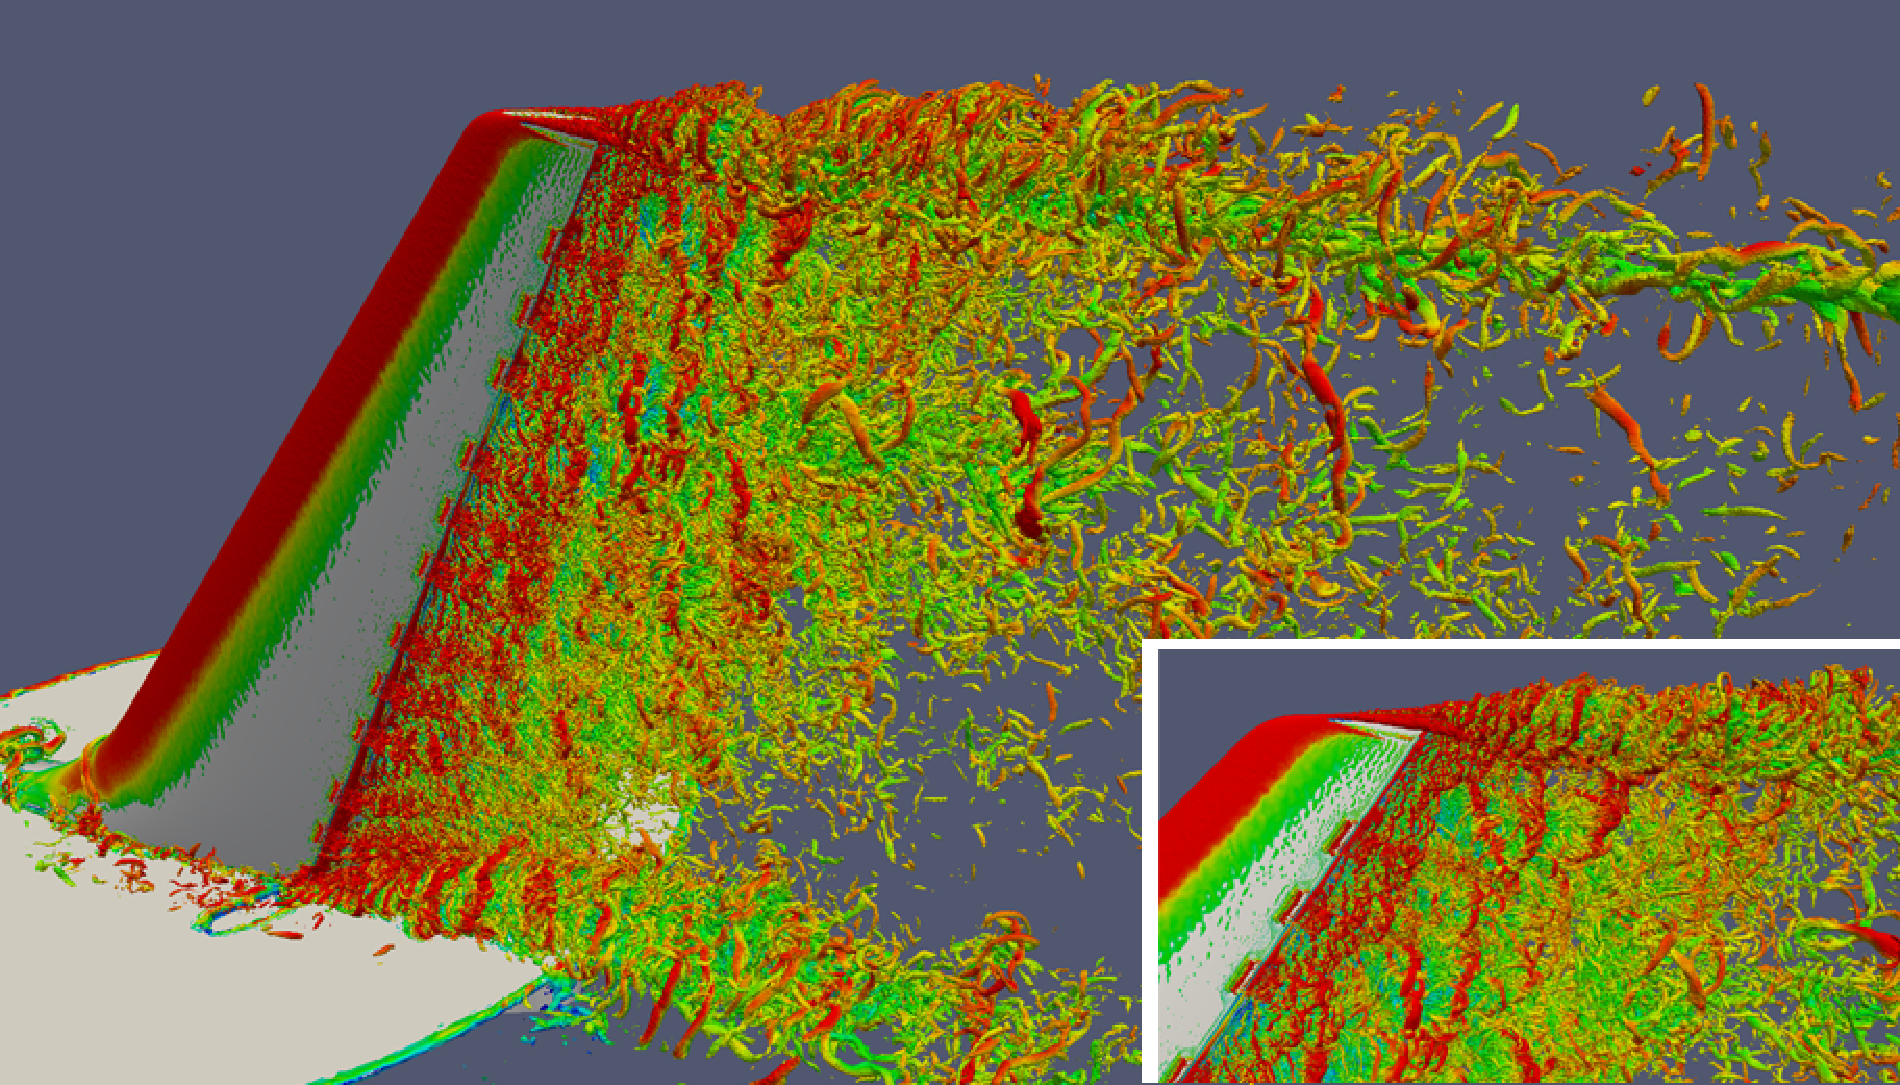
\includegraphics[width=0.517\linewidth]{images/WingWake}
  \end{tabular}
  \parbox{0.95\linewidth}{\footnotesize ParaView visualizations run in situ with large scale \href{https://phasta.scigap.org/}{\bf\underline{PHASTA}} simulations
  
  \newline\vskip 6pt
  
  {\bf Left} \quad 3.3 billion tetrahedral mesh simulating the flow over a full wing where a synthetic jet issues an unsteady crossflow jet (run on 160 thousand MPI processes)
  
  \newline\vskip 6pt
  
  {\bf Right} \quad is a 1.3 billion element mesh simulating the wake of a deflected wing flap (run on 256 thousand MPI processes)}
  
\end{inlinefig}
    
\end{frame}{}

\begin{frame}{Exercise}

Read parallel visualization algorithms and parallel rendering in Chapter 4 of the tutorials

\vskip 12pt

Paraview tutorial exercise 4.1

\end{frame}{}

\section{Evaluation}

\begin{frame}{Evaluation}
    
Evaluation exercise using scientific data:
\begin{itemize}
    \item Choose from given OpenFOAM tutorials. All students must use different data
    \item Create images, videos, etc then put in document (good formatting, e.g. correct font sizes, etc)
\end{itemize}{}
    
    Marks awarded for:
    \begin{description}{}
        \item[3-D] visualisations using filters % 20%
        \item[Line plots] extracted from 3-D data % 20%
        \item[Animation] showing instructive behaviour % 20%
        \item[Description] of interesting behaviour % 30%
        \item[Formatting] i.e. layout, colour choices, font sizes, etc % 10%
    \end{description}
    
\end{frame}{}

\begin{frame}{Evaluation hints}

Do \underline{not} include screen captures.

\vskip 12 pt

No visualisations without filters applied.

\vskip 12 pt

Add axis labels to line charts.

\vskip 12 pt

Add annotation to movie; e.g. time, title, etc.

\vskip 12 pt

Document in \underline{pdf} format and separate movie file.

\vskip 12 pt

Only \underline{one} animation. Use multi-view if necessary.

\vskip 12 pt

Best marks for comparisons involving superimposed statistics

\end{frame}{}

%\begin{frame}{Data representations : Glyph}
    
%\end{frame}{}

%\begin{frame}{Data representations : Streamlines}
    
%\end{frame}{}

%\begin{frame}{Data representations : Isosurface}
    
%\end{frame}{}

%\begin{frame}{Data representations : Slices}
    
%\end{frame}{}

\end{document}
